\newpage
%***********************************************************************************
\section{Forward Uncertainty Propagation of MCMC samples}\label{app:mcmc_evaluation}
%***********************************************************************************

%-----------------------------------------------------------------------------------------------------
\subsection{FEBA Test No. 216, clad Temperature Output (TC)}\label{app:tbl_results_uq_post_tc_216}
%-----------------------------------------------------------------------------------------------------

% FEBA Test No. 216 Posterior Uncertainty Propagation, TC, with model bias term
\rotatebox{90}{\begin{minipage}{0.85\textheight}
    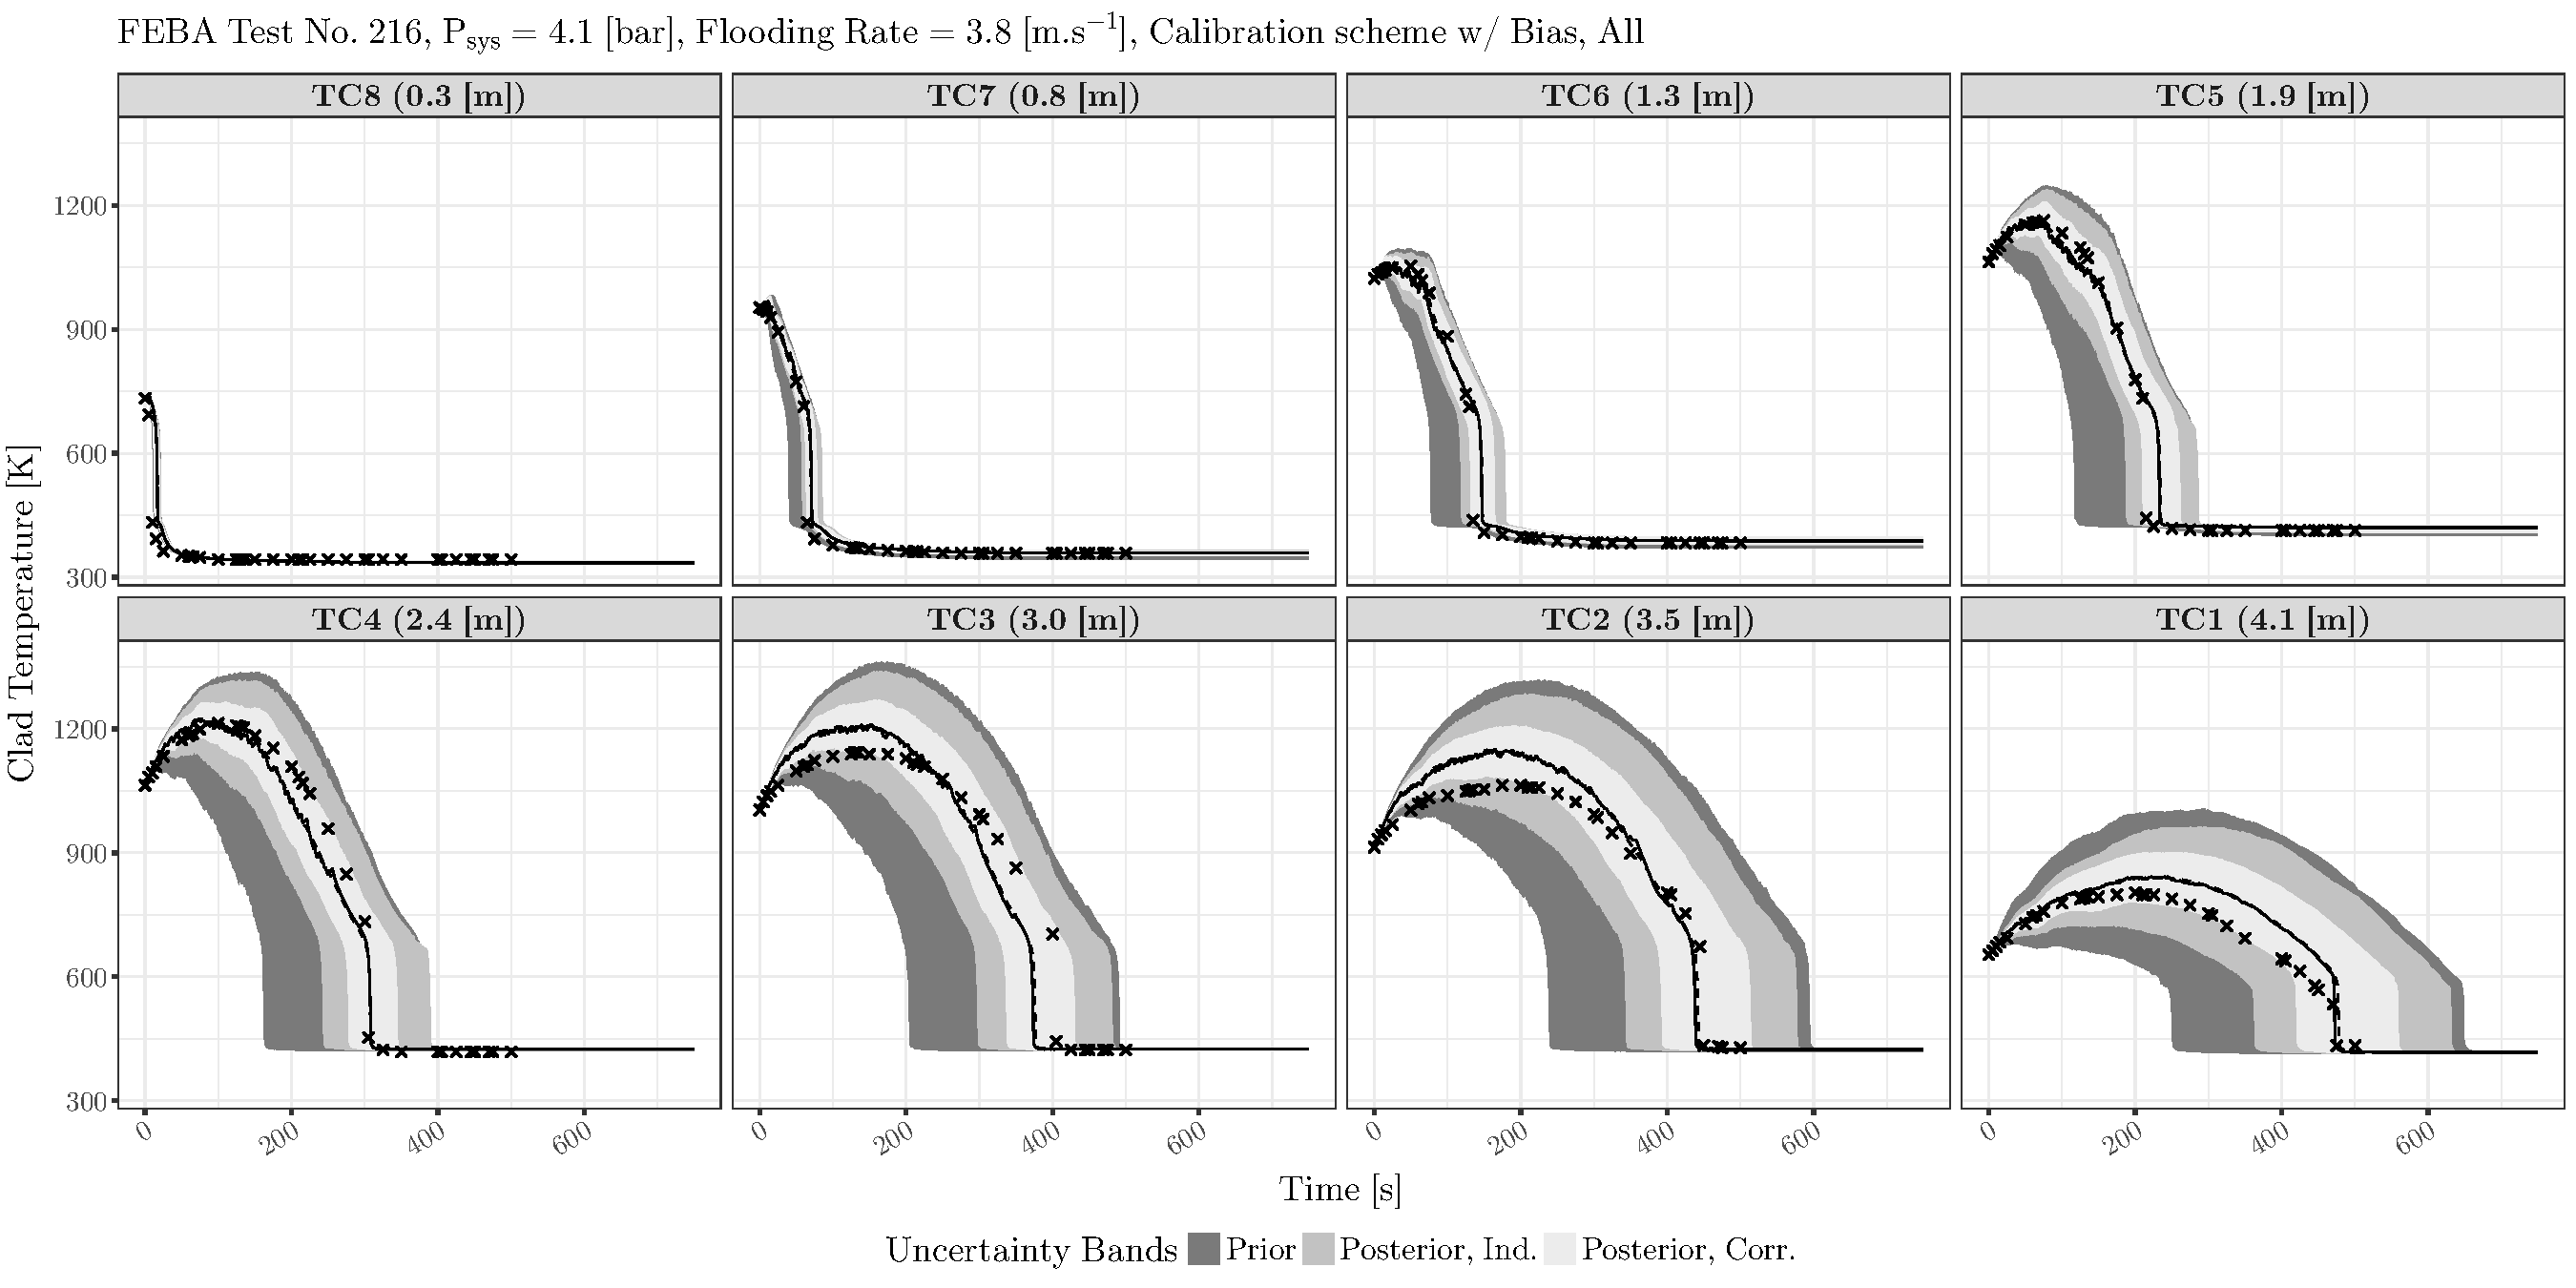
\includegraphics[width=0.95\textwidth]{../figures/chapter5/figures/plotTraceUQPosteriorAllDiscCenteredTC216}
		\captionof{figure}[Propagation of the model parameters uncertainty on FEBA test No. $216$ for the clad temperature output ($TC$). The posterior samples are from the calibration scheme \texttt{w/ Bias, All}.]{Propagation of the model parameters uncertainty on FEBA test No. $216$ for the clad temperature output ($TC$) at different axial locations. The uncertainty bands refer to the symmetric $95\%$ probabilities. Solid lines, dashed lines, and crosses indicate the simulation with the nominal parameters values, the median of the posterior, and the experimental data, respectively. The posterior samples are from the calibration with model bias term and considering all types of output (\texttt{w/ Bias, All}).}
    \label{fig:ch5_app_plot_trace_uq_post_tc_216_disc}
\end{minipage}}

% FEBA Test No. 216 Posterior Uncertainty Propagation, TC, without Parameter 8
\clearpage
\begin{sidewaysfigure}
	\centering
	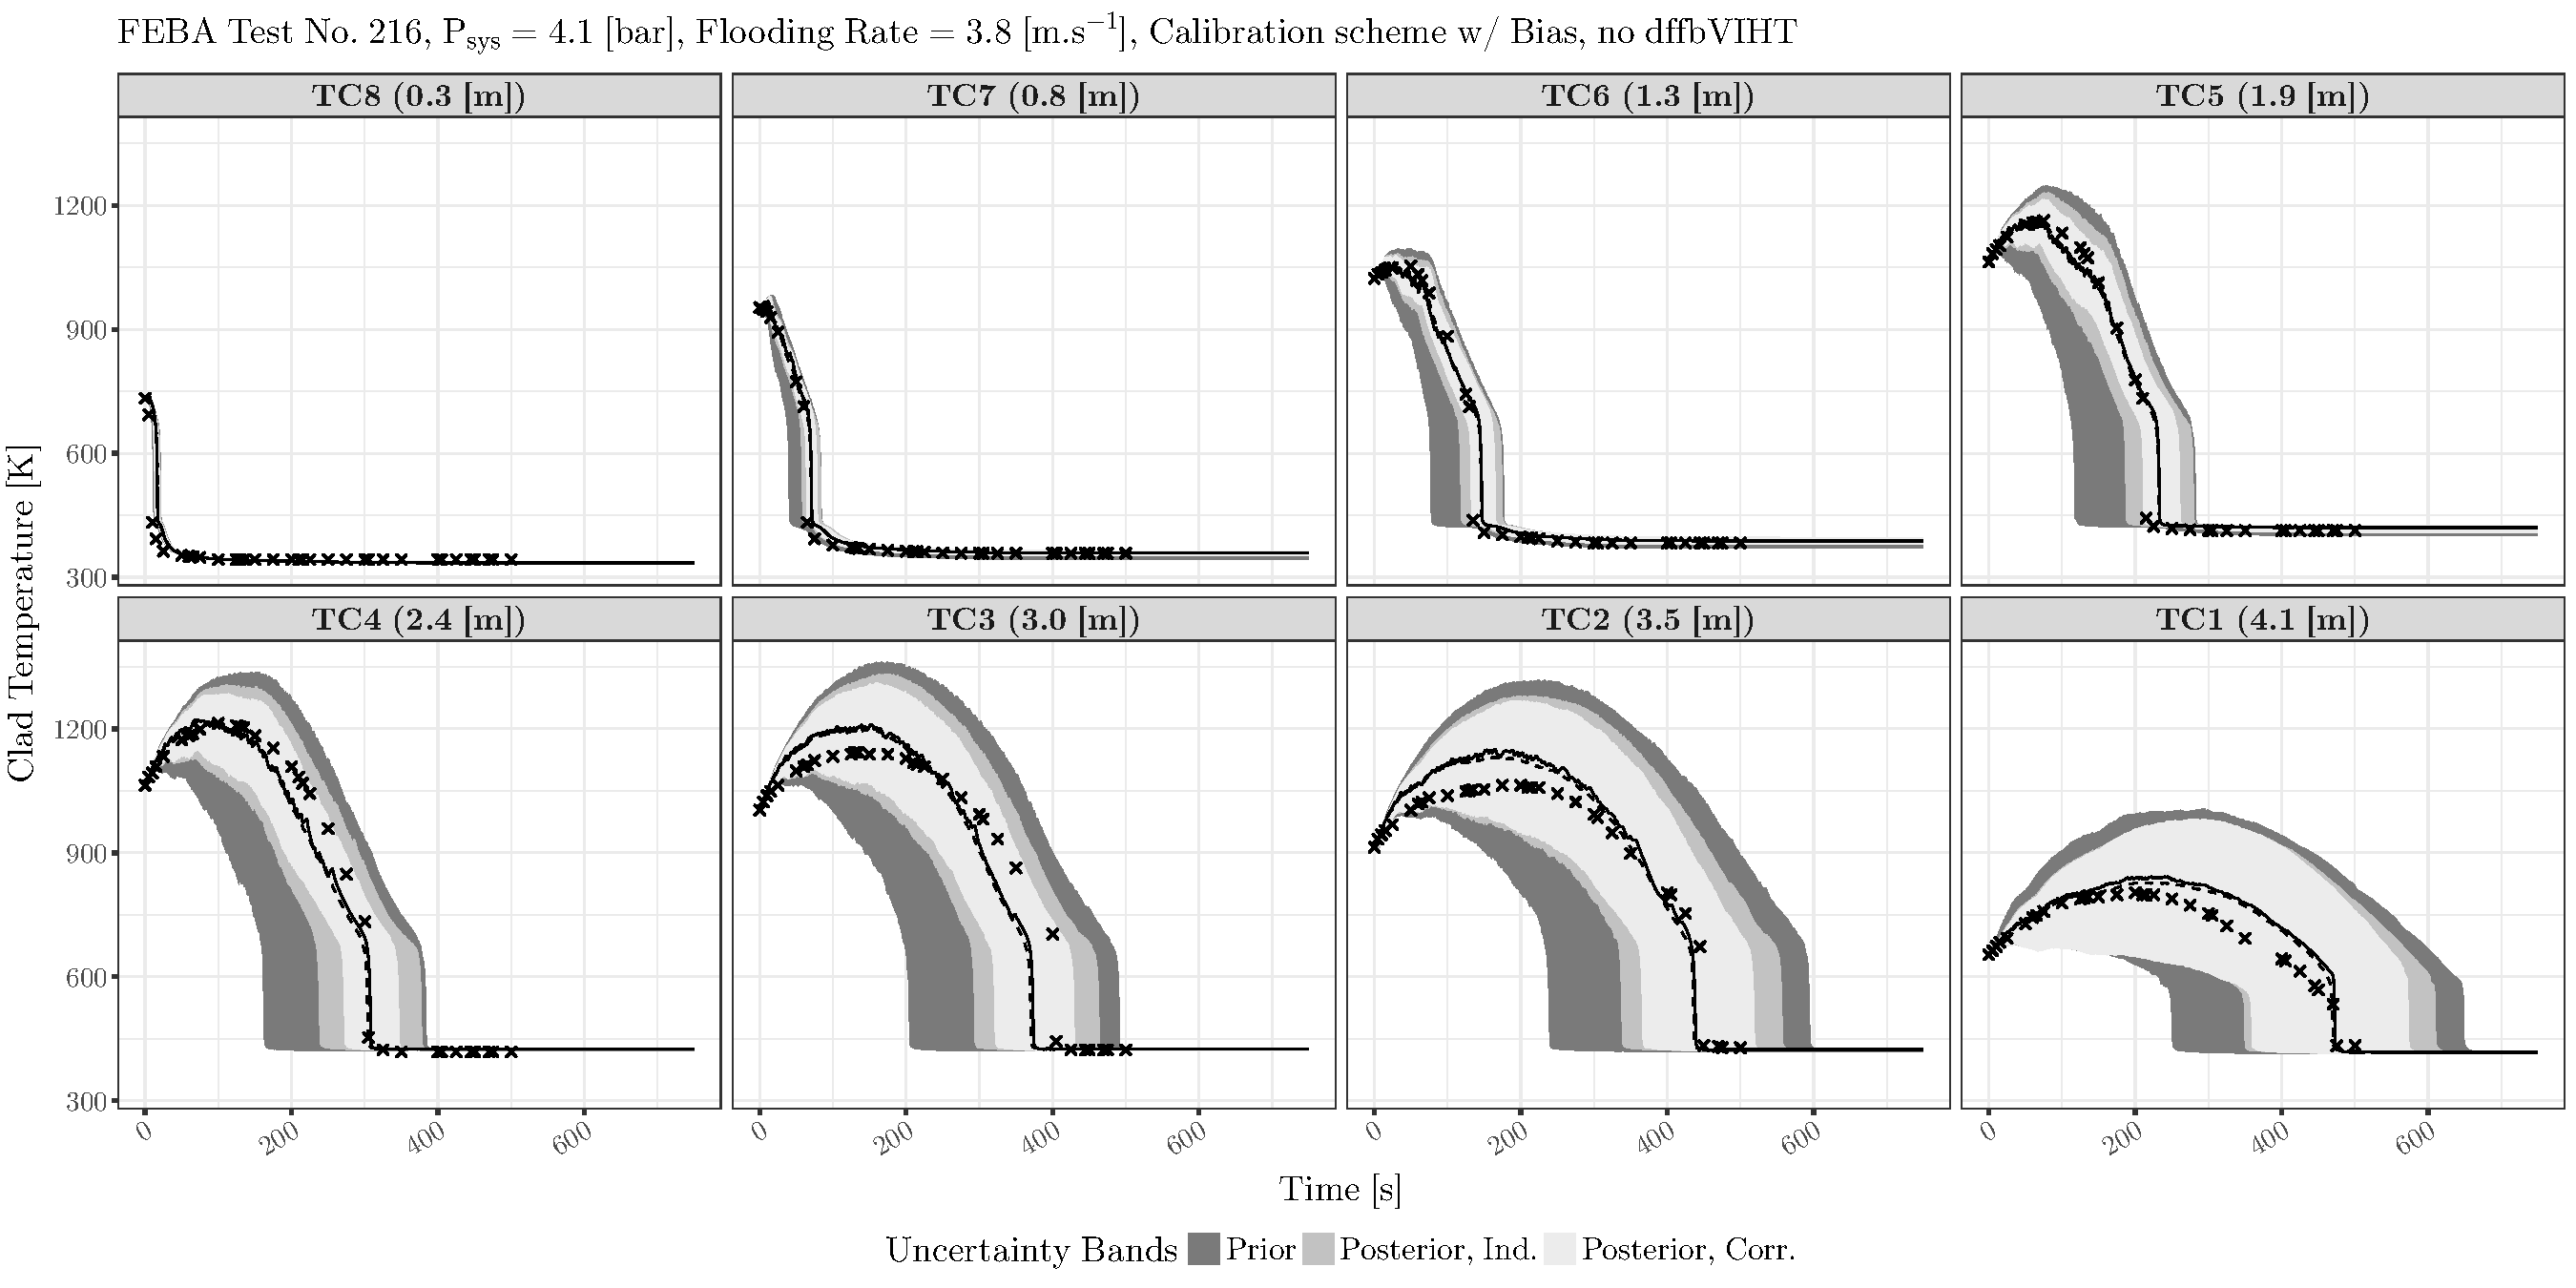
\includegraphics[width=0.90\textwidth]{../figures/chapter5/figures/plotTraceUQPosteriorAllDiscCenteredNoParam8TC216}
		\captionof{figure}[Propagation of the model parameters uncertainty on FEBA test No. $216$ for the clad temperature output ($TC$). The posterior samples are from the calibration scheme \texttt{w/ Bias, no dffbVIHT}.]{Propagation of the model parameters uncertainty on FEBA test No. $216$ for the clad temperature output ($TC$) at different axial locations. The uncertainty bands refer to the symmetric $95\%$ probabilities. Solid lines, dashed lines, and crosses indicate the simulation with the nominal parameters values, the median of the posterior, and the experimental data, respectively. The posterior samples are from the calibration with model bias term, considering all types of output, but excluding the parameter \texttt{dffbVIHT} (\texttt{w/ Bias, no dffbVIHT}).}
	\label{fig:ch5_plot_trace_uq_post_tc_216_noparam8}
\end{sidewaysfigure}
\clearpage

% FEBA Test No. 216 Posterior Uncertainty Propagation, TC, without model bias term
\clearpage
\begin{sidewaysfigure}
	\centering
	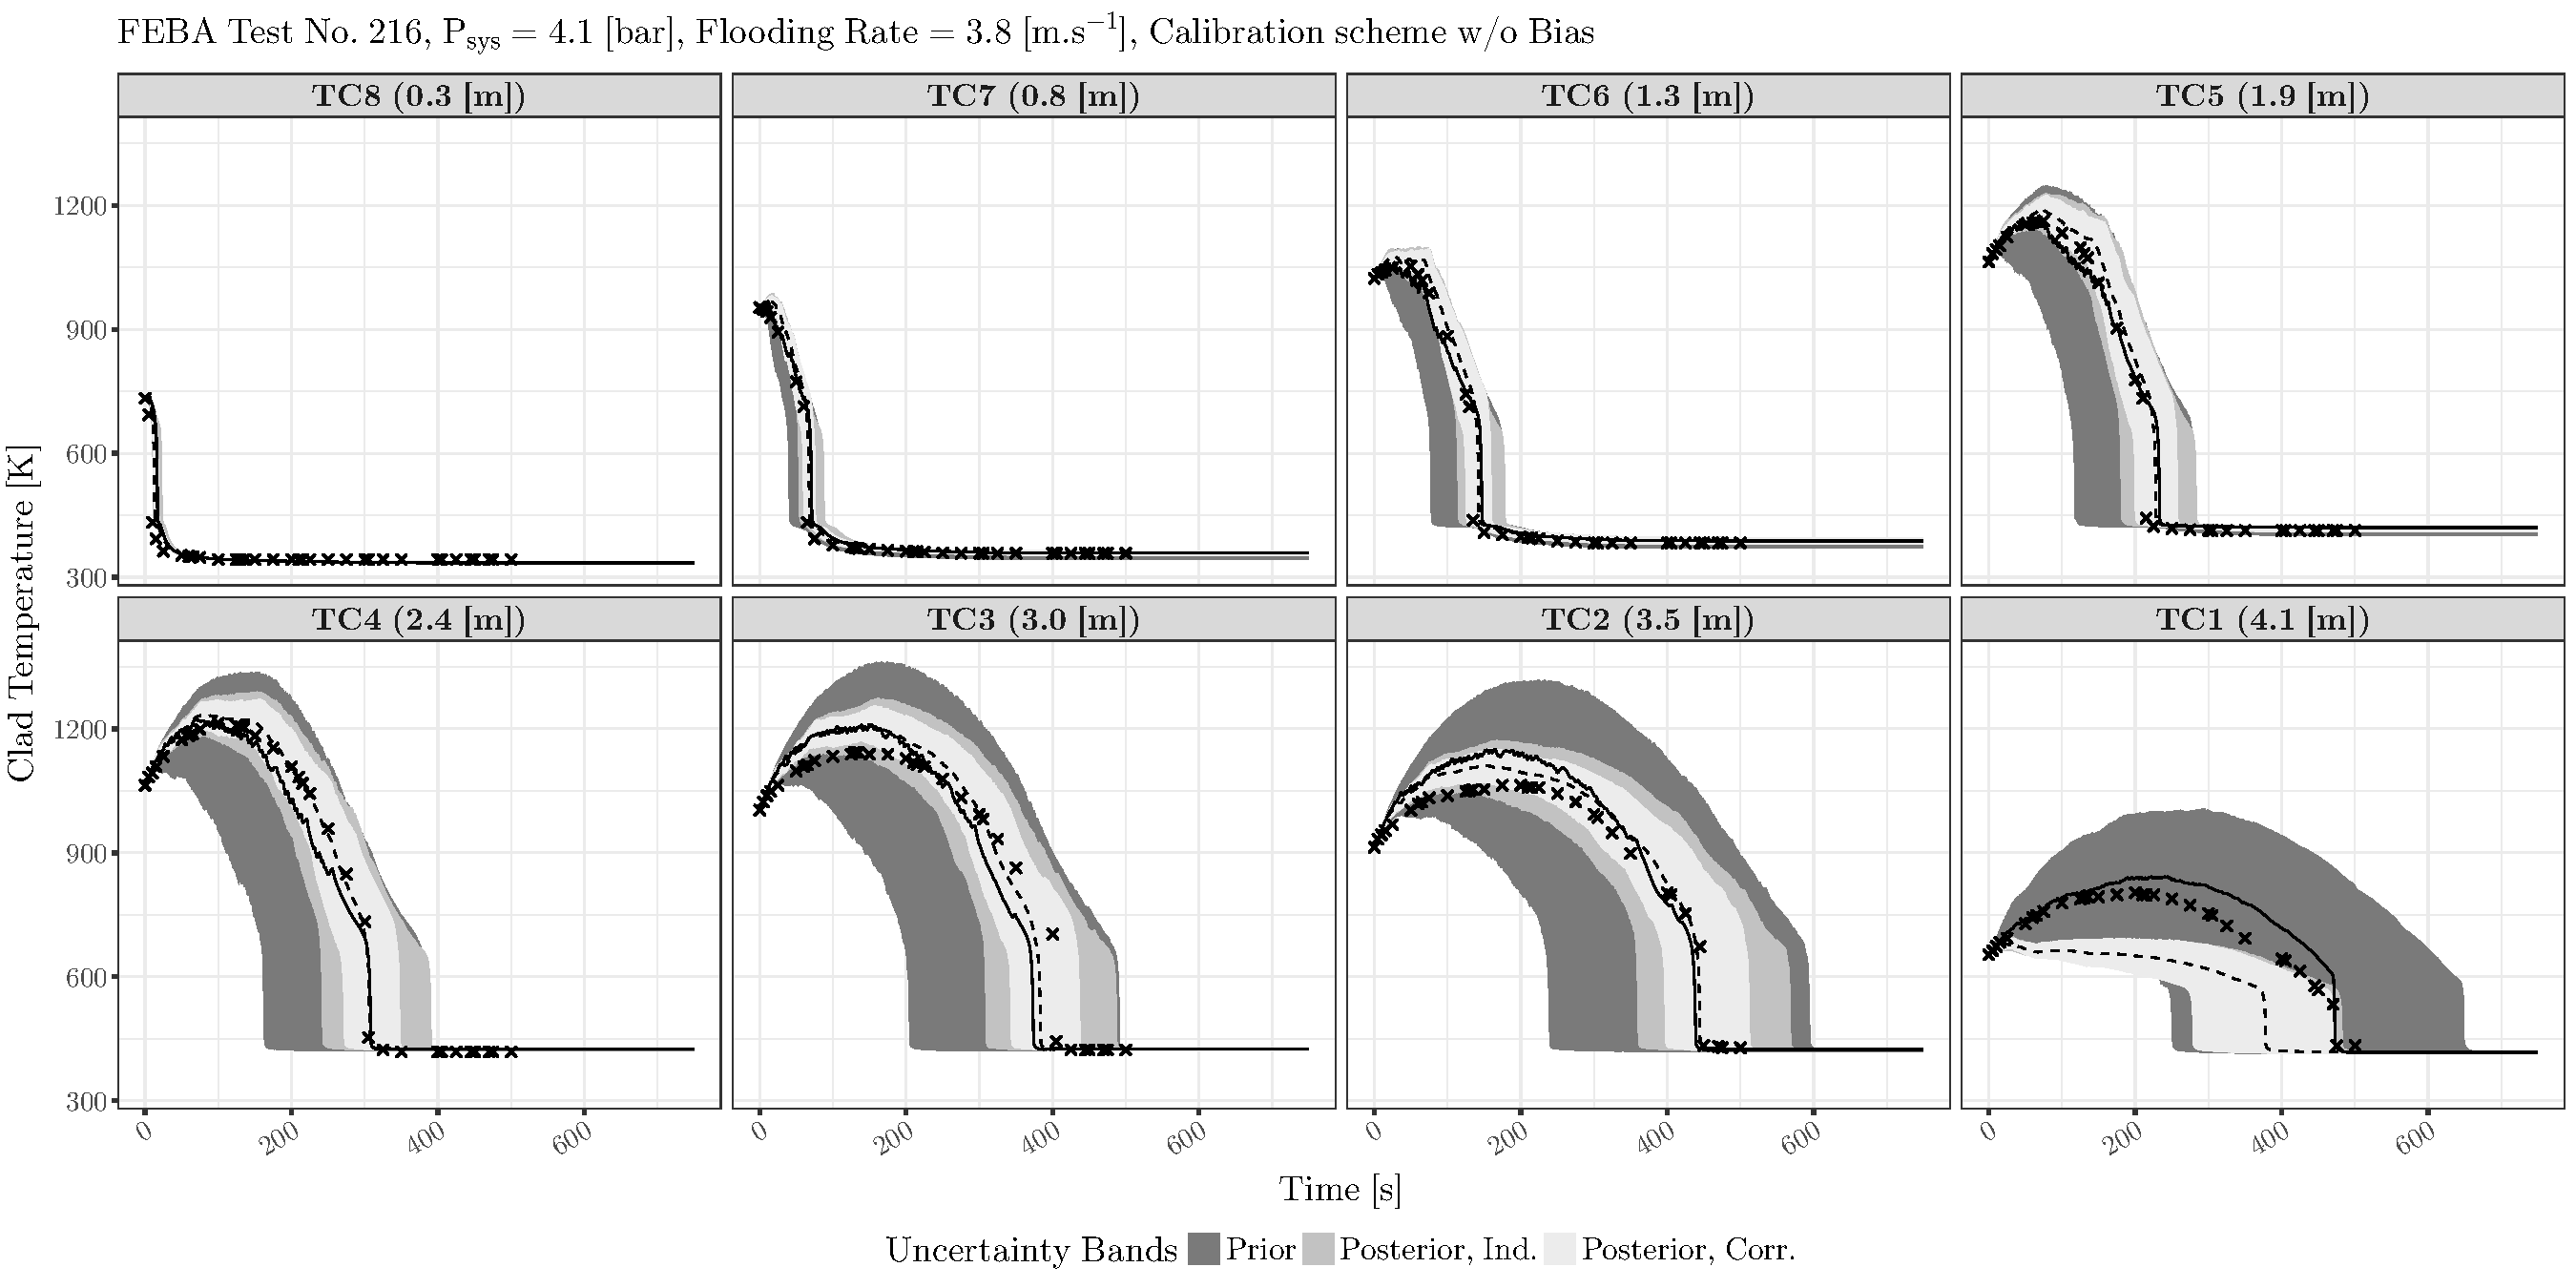
\includegraphics[width=0.90\textwidth]{../figures/chapter5/figures/plotTraceUQPosteriorAllNoDiscNoBCTC216}
		\captionof{figure}[Posterior uncertainty propagation of FEBA test No. $216$ for the clad temperature output ($TC$). The posterior samples are from the calibration scheme \texttt{w/o Bias}.]{Propagation of the model parameters uncertainty on FEBA test No. $216$ for the clad temperature output ($TC$) at different axial locations. The uncertainty bands refer to the symmetric $95\%$ probabilities. Solid lines, dashed lines, and crosses indicate the simulation with the nominal parameters values, the median of the posterior, and the experimental data, respectively. The posterior samples are from the calibration without model bias term and considering all types of output (\texttt{w/o Bias}).}
	\label{fig:ch5_plot_trace_uq_post_tc_216_nodisc}
\end{sidewaysfigure}
\clearpage

%-----------------------------------------------------------------------------------------------------
\subsection{FEBA Test No. 214, clad Temperature Output (TC)}\label{app:tbl_results_uq_post_tc_214}
%-----------------------------------------------------------------------------------------------------

% FEBA Test No. 214 Posterior Uncertainty Propagation, TC, with model bias term
\rotatebox{90}{\begin{minipage}{0.85\textheight}
    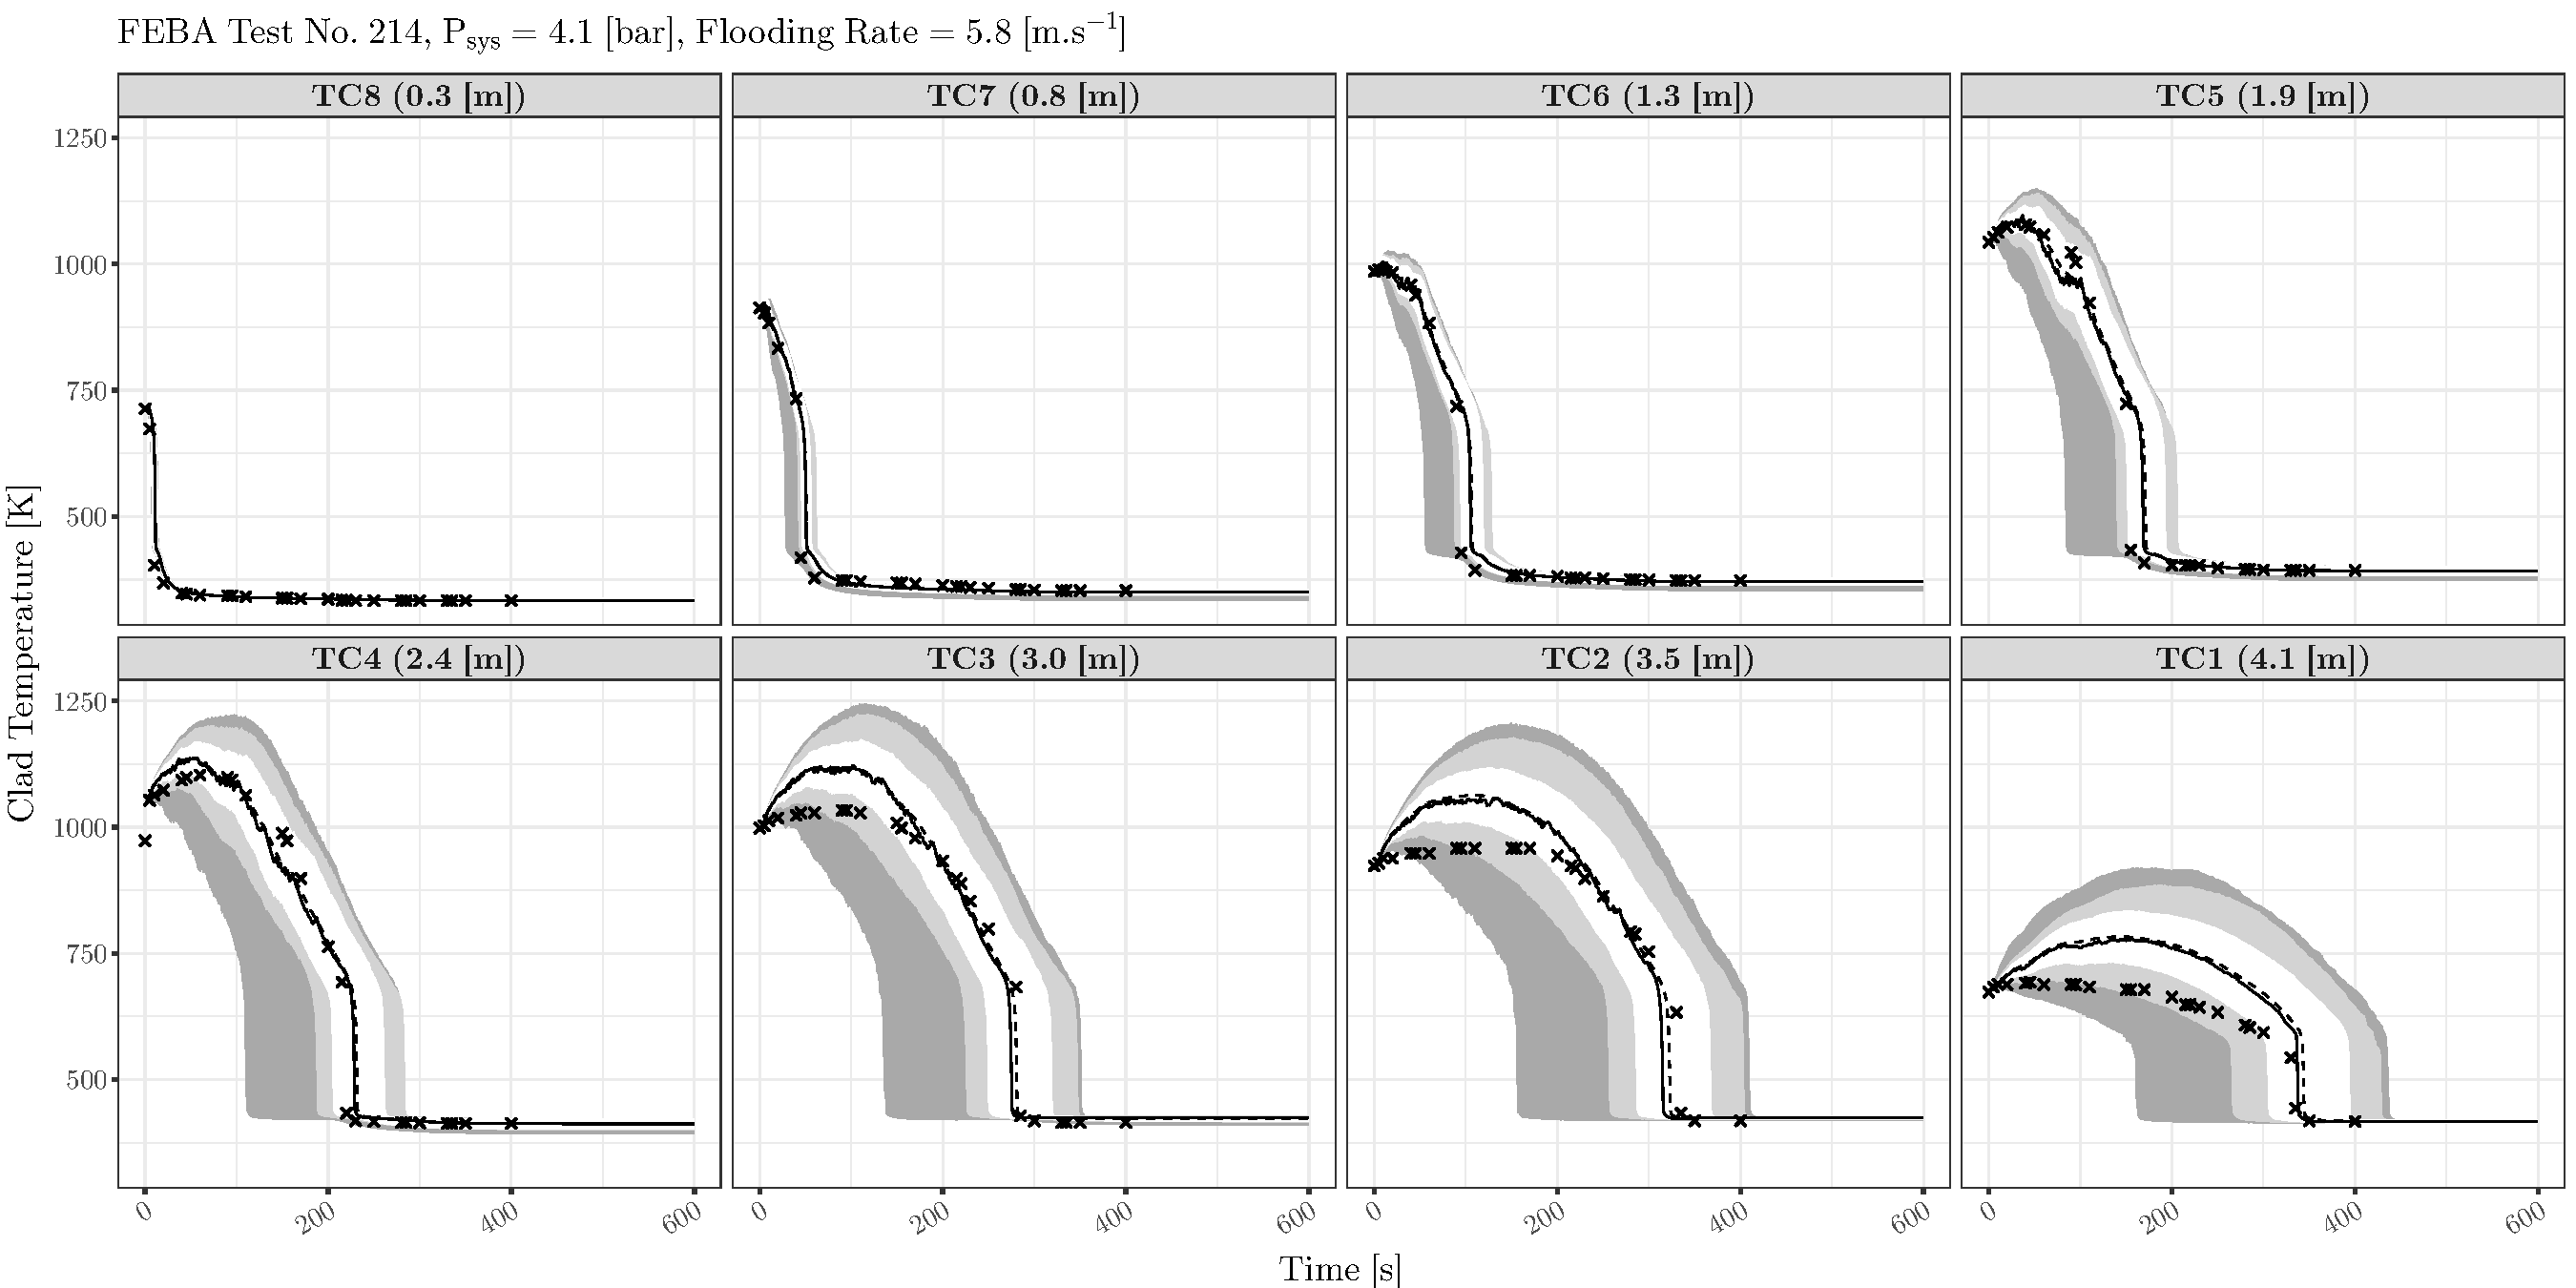
\includegraphics[width=0.95\textwidth]{../figures/chapter5/figures/plotTraceUQPosteriorAllDiscCenteredTC214}
		\captionof{figure}[Propagation of the model parameters uncertainty on FEBA test No. $214$ for the clad temperature output ($TC$). The posterior samples are from the calibration scheme \texttt{w/ Bias, All}.]{Propagation of the model parameters uncertainty on FEBA test No. $214$ for the clad temperature output ($TC$) at different axial locations. The uncertainty bands refer to the symmetric $95\%$ probabilities. Solid lines, dashed lines, and crosses indicate the simulation with the nominal parameters values, the median of the posterior, and the experimental data, respectively. The posterior samples are from the calibration with model bias term and considering all types of output (\texttt{w/ Bias, All}).}
    \label{fig:ch5_plot_trace_uq_post_tc_214_disc}
\end{minipage}}

% FEBA Test No. 214 Posterior Uncertainty Propagation, TC, without Parameter 8
\clearpage
\begin{sidewaysfigure}
	\centering
	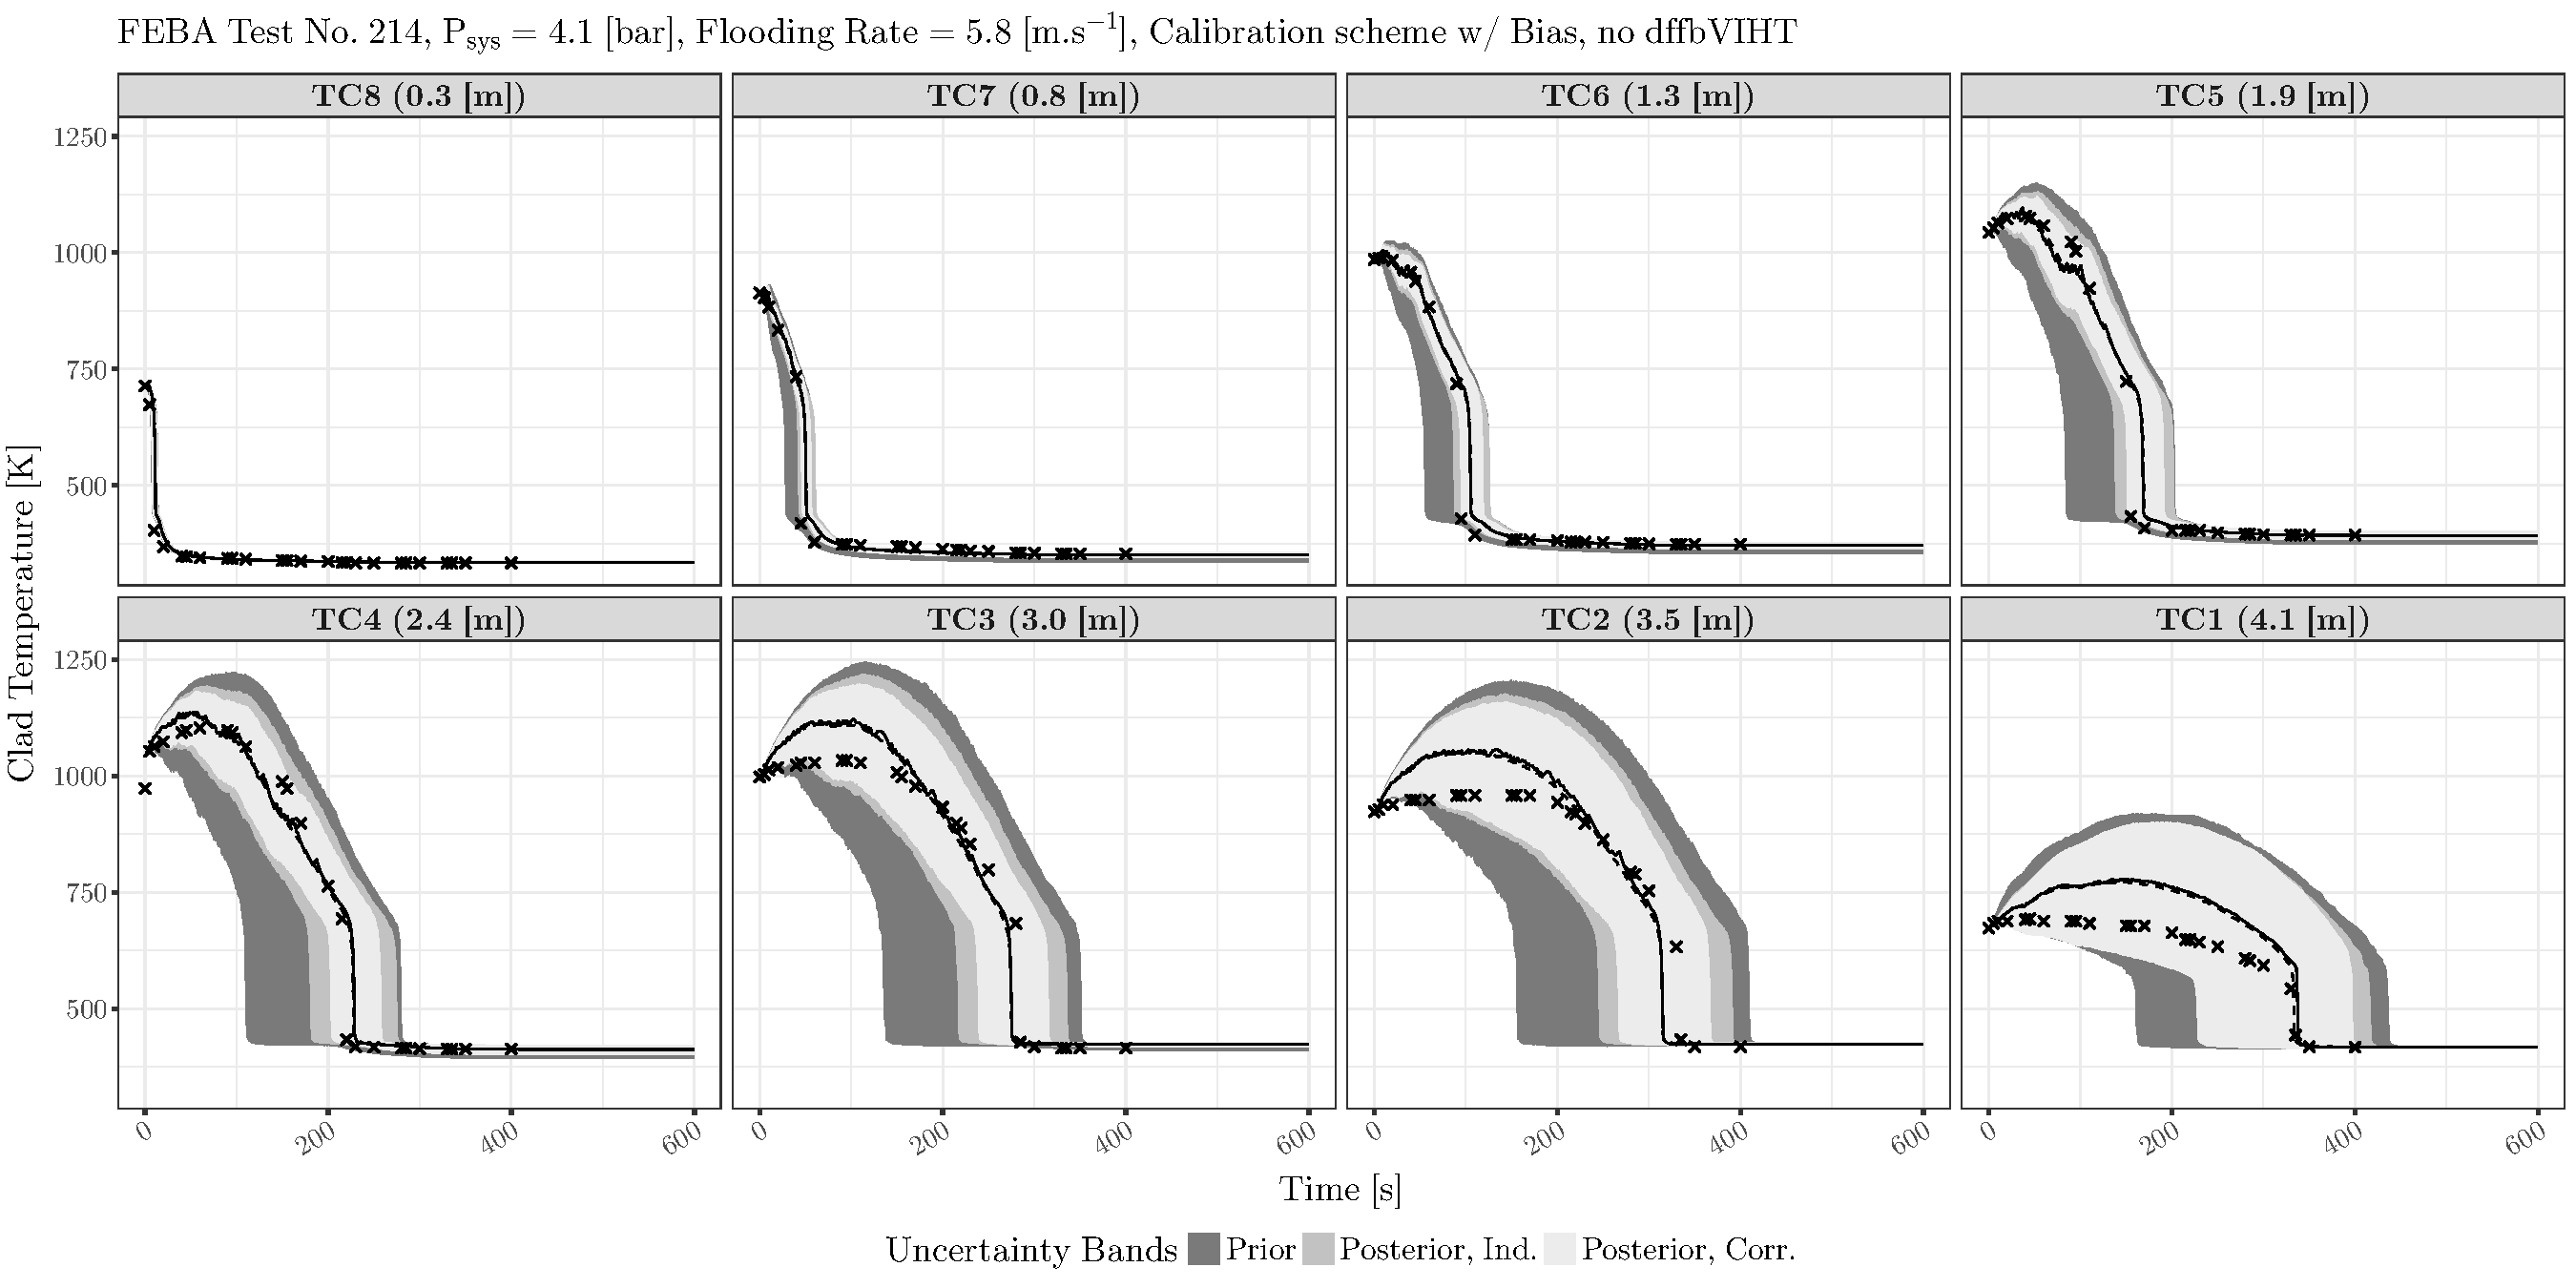
\includegraphics[width=0.90\textwidth]{../figures/chapter5/figures/plotTraceUQPosteriorAllDiscCenteredNoParam8TC214}
		\captionof{figure}[Propagation of the model parameters uncertainty on FEBA test No. $214$ for the clad temperature output ($TC$). The posterior samples are from the calibration scheme \texttt{w/ Bias, no dffbVIHT}.]{Propagation of the model parameters uncertainty on FEBA test No. $214$ for the clad temperature output ($TC$) at different axial locations. The uncertainty bands refer to the symmetric $95\%$ probabilities. Solid lines, dashed lines, and crosses indicate the simulation with the nominal parameters values, the median of the posterior, and the experimental data, respectively. The posterior samples are from the calibration with model bias term, considering all types of output, but excluding the parameter \texttt{dffbVIHT} (\texttt{w/ Bias, no dffbVIHT}).}
	\label{fig:ch5_plot_trace_uq_post_tc_214_noparam8}
\end{sidewaysfigure}
\clearpage

% FEBA Test No. 214 Posterior Uncertainty Propagation, TC, without model bias term
\clearpage
\begin{sidewaysfigure}
	\centering
	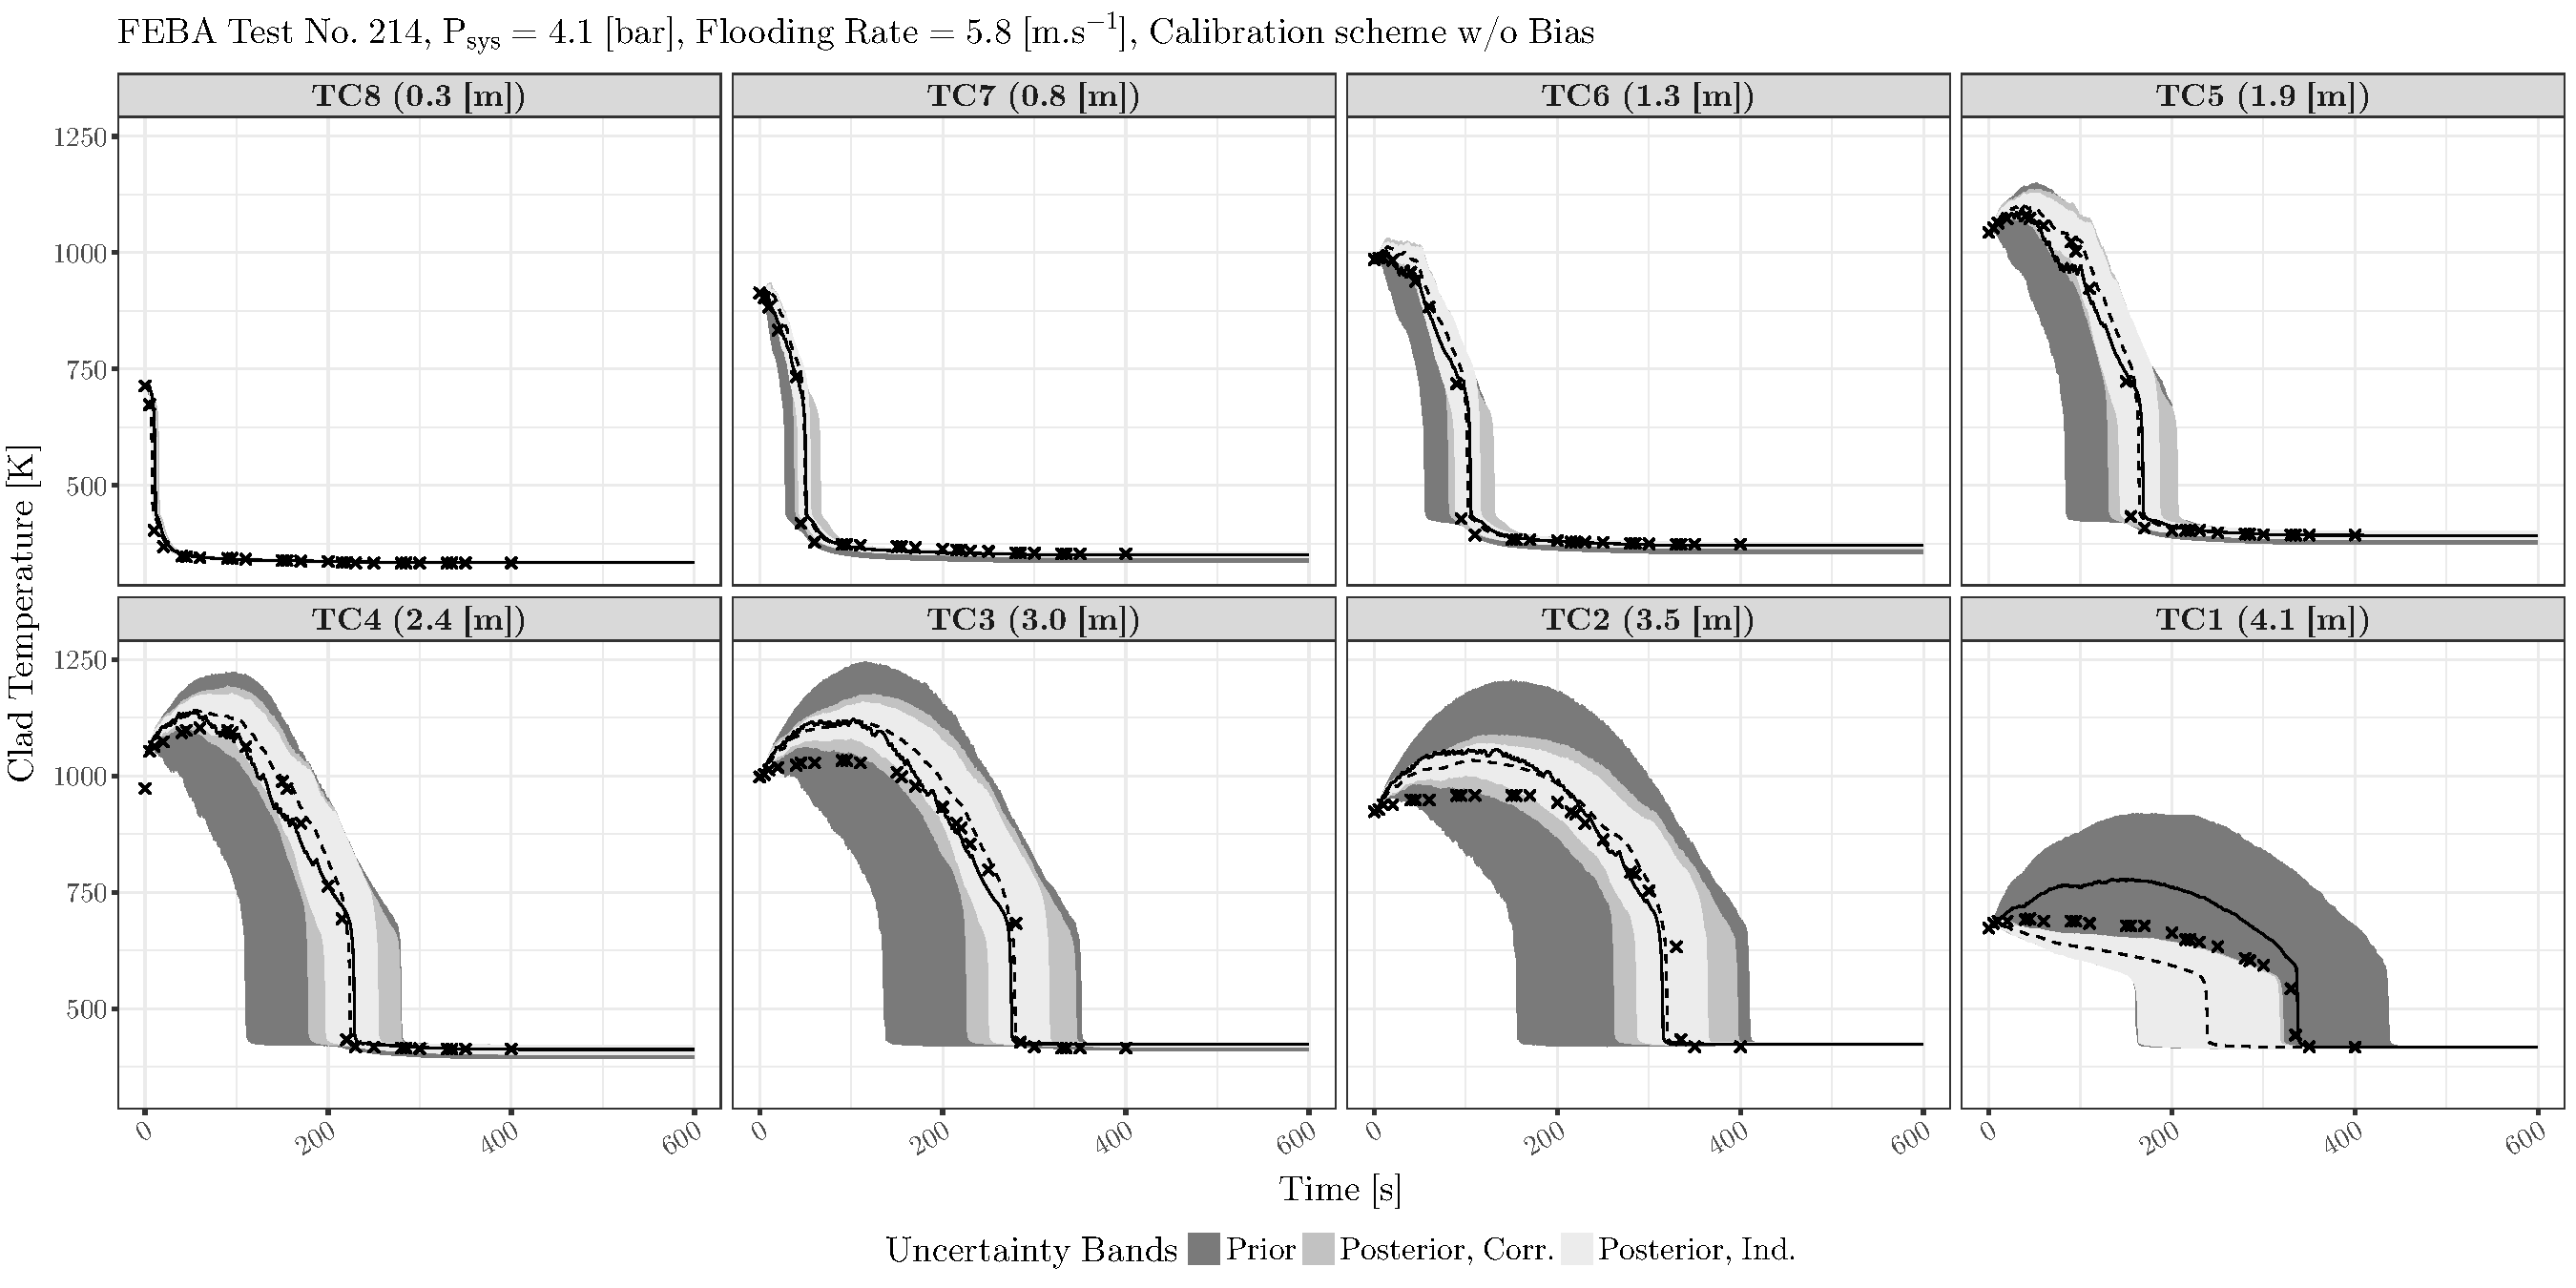
\includegraphics[width=0.90\textwidth]{../figures/chapter5/figures/plotTraceUQPosteriorAllNoDiscNoBCTC214}
		\captionof{figure}[Posterior uncertainty propagation of FEBA test No. $214$ for the clad temperature output ($TC$). The posterior samples are from the calibration scheme \texttt{w/o Bias}.]{Propagation of the model parameters uncertainty on FEBA test No. $214$ for the clad temperature output ($TC$) at different axial locations. The uncertainty bands refer to the symmetric $95\%$ probabilities. Solid lines, dashed lines, and crosses indicate the simulation with the nominal parameters values, the median of the posterior, and the experimental data, respectively. The posterior samples are from the calibration without model bias term and considering all types of output (\texttt{w/o Bias}).}
	\label{fig:ch5_plot_trace_uq_post_tc_214_nodisc}
\end{sidewaysfigure}
\clearpage

%-----------------------------------------------------------------------------------------------------
\subsection{FEBA Test No. 223, clad Temperature Output (TC)}\label{app:tbl_results_uq_post_tc_223}
%-----------------------------------------------------------------------------------------------------

% FEBA Test No. 223 Posterior Uncertainty Propagation, TC, with model bias term
\rotatebox{90}{\begin{minipage}{0.85\textheight}
    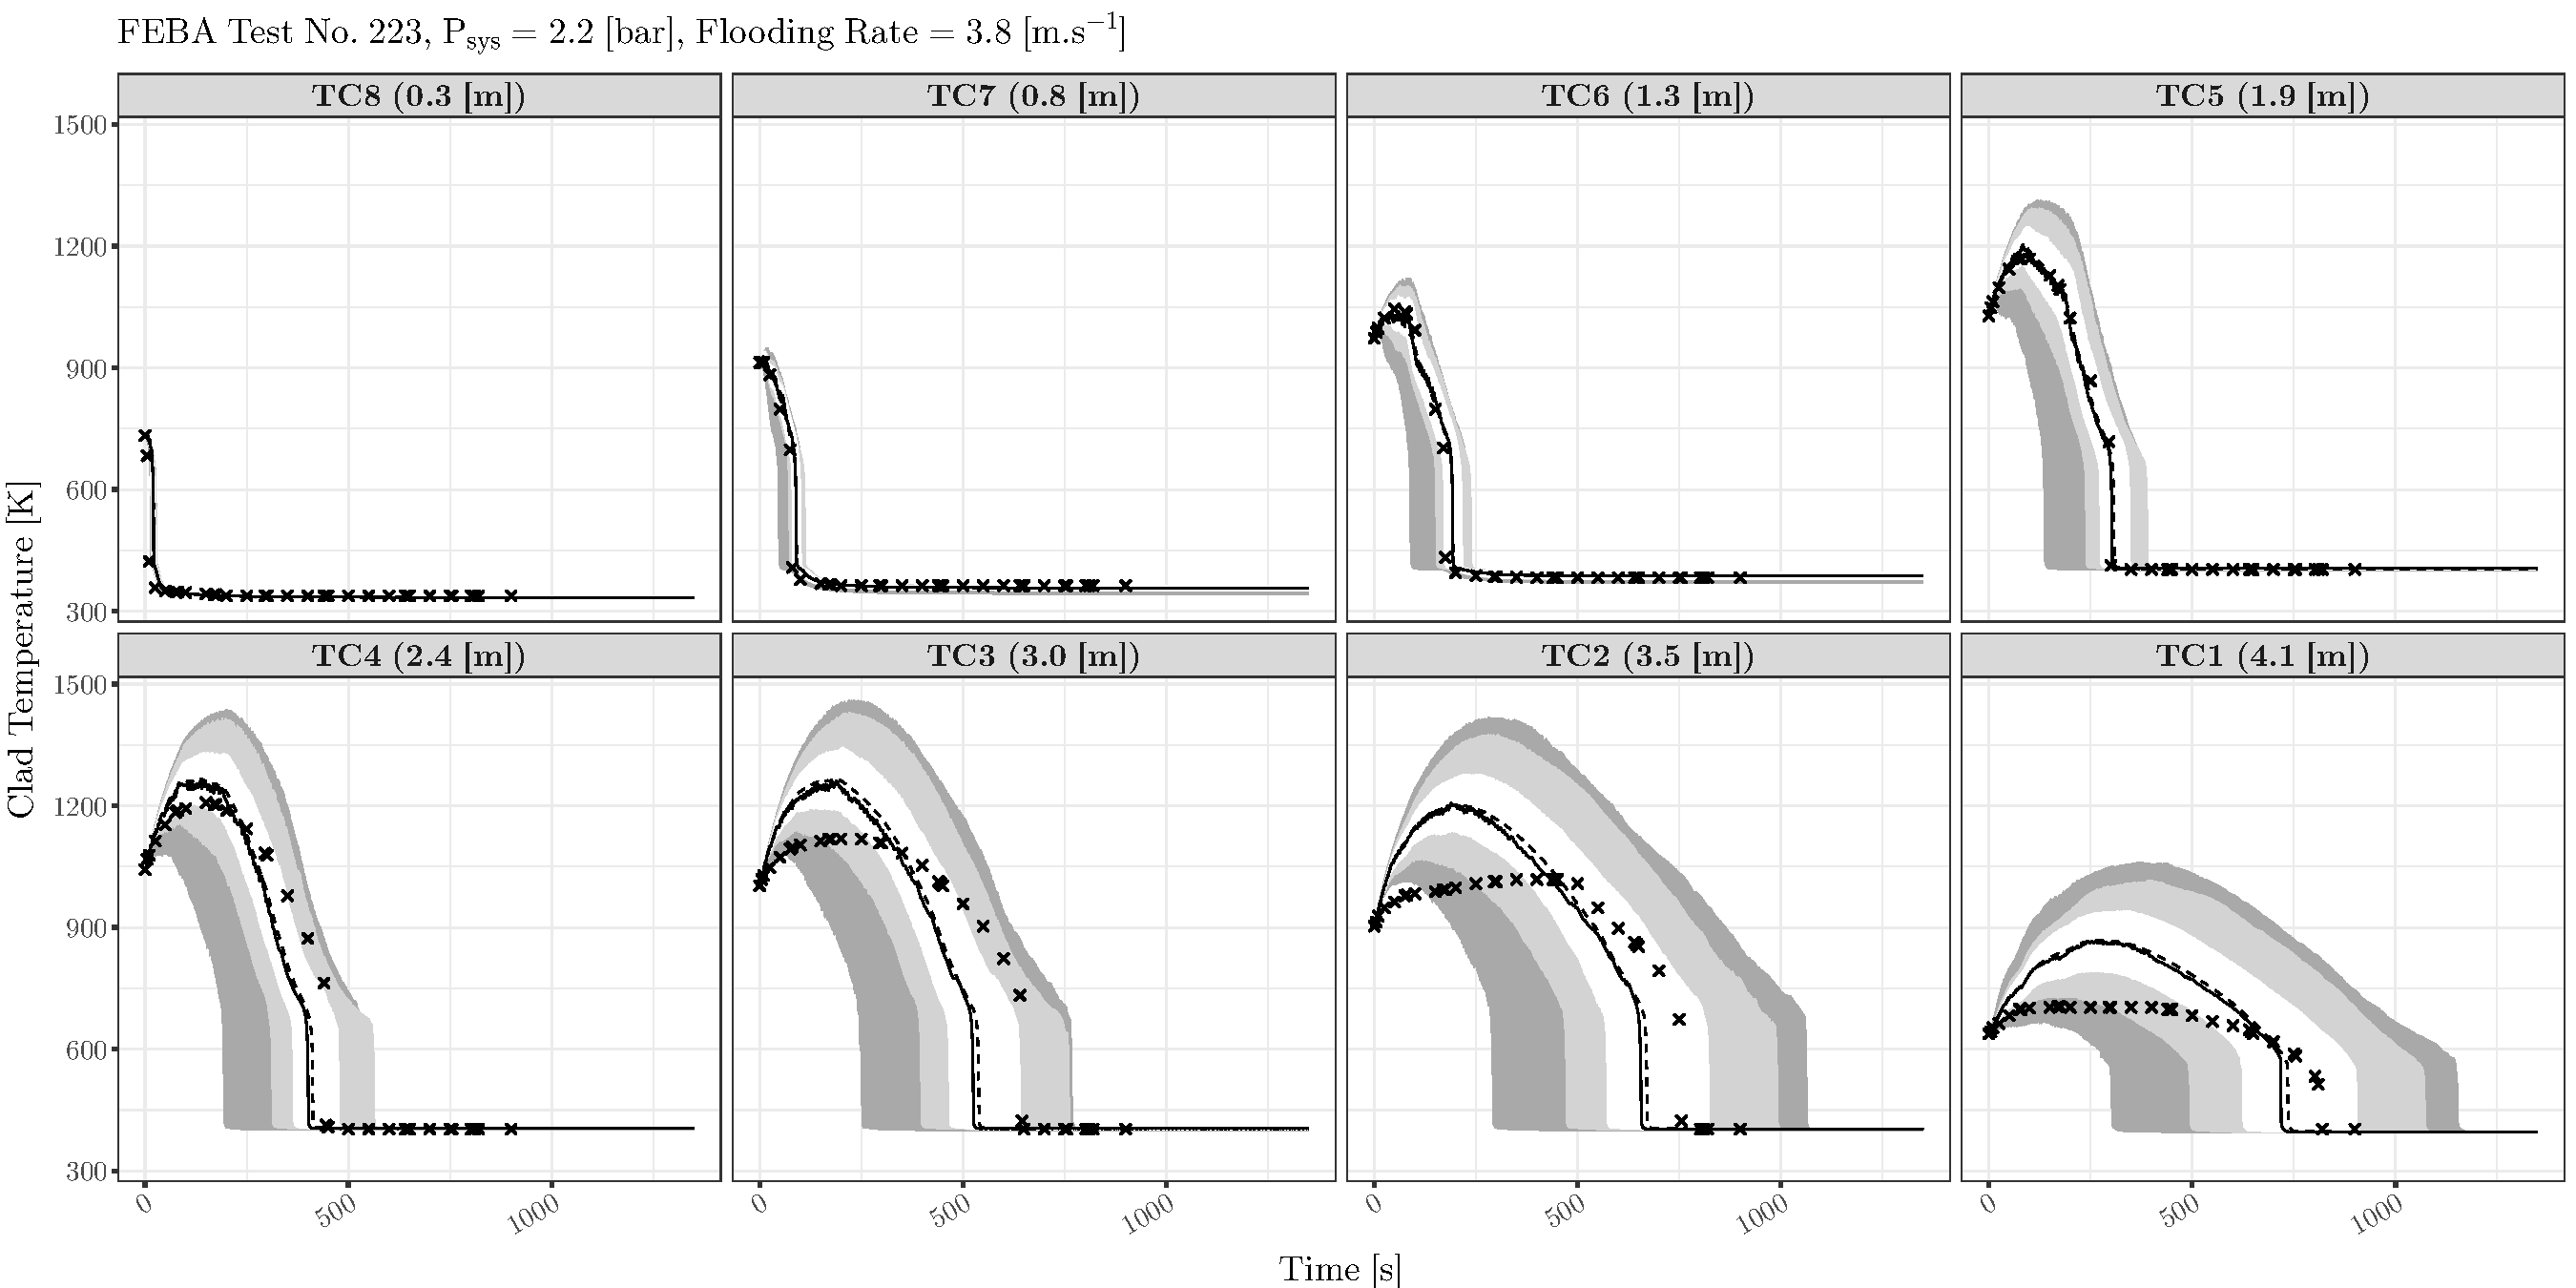
\includegraphics[width=0.95\textwidth]{../figures/chapter5/figures/plotTraceUQPosteriorAllDiscCenteredTC223}
		\captionof{figure}[Propagation of the model parameters uncertainty on FEBA test No. $223$ for the clad temperature output ($TC$). The posterior samples are from the calibration scheme \texttt{w/ Bias, All}.]{Propagation of the model parameters uncertainty on FEBA test No. $223$ for the clad temperature output ($TC$) at different axial locations. The uncertainty bands refer to the symmetric $95\%$ probabilities. Solid lines, dashed lines, and crosses indicate the simulation with the nominal parameters values, the median of the posterior, and the experimental data, respectively. The posterior samples are from the calibration with model bias term and considering all types of output (\texttt{w/ Bias, All}).}
    \label{fig:ch5_plot_trace_uq_post_tc_223_disc}
\end{minipage}}

% FEBA Test No. 223 Posterior Uncertainty Propagation, TC, without Parameter 8
\clearpage
\begin{sidewaysfigure}
	\centering
	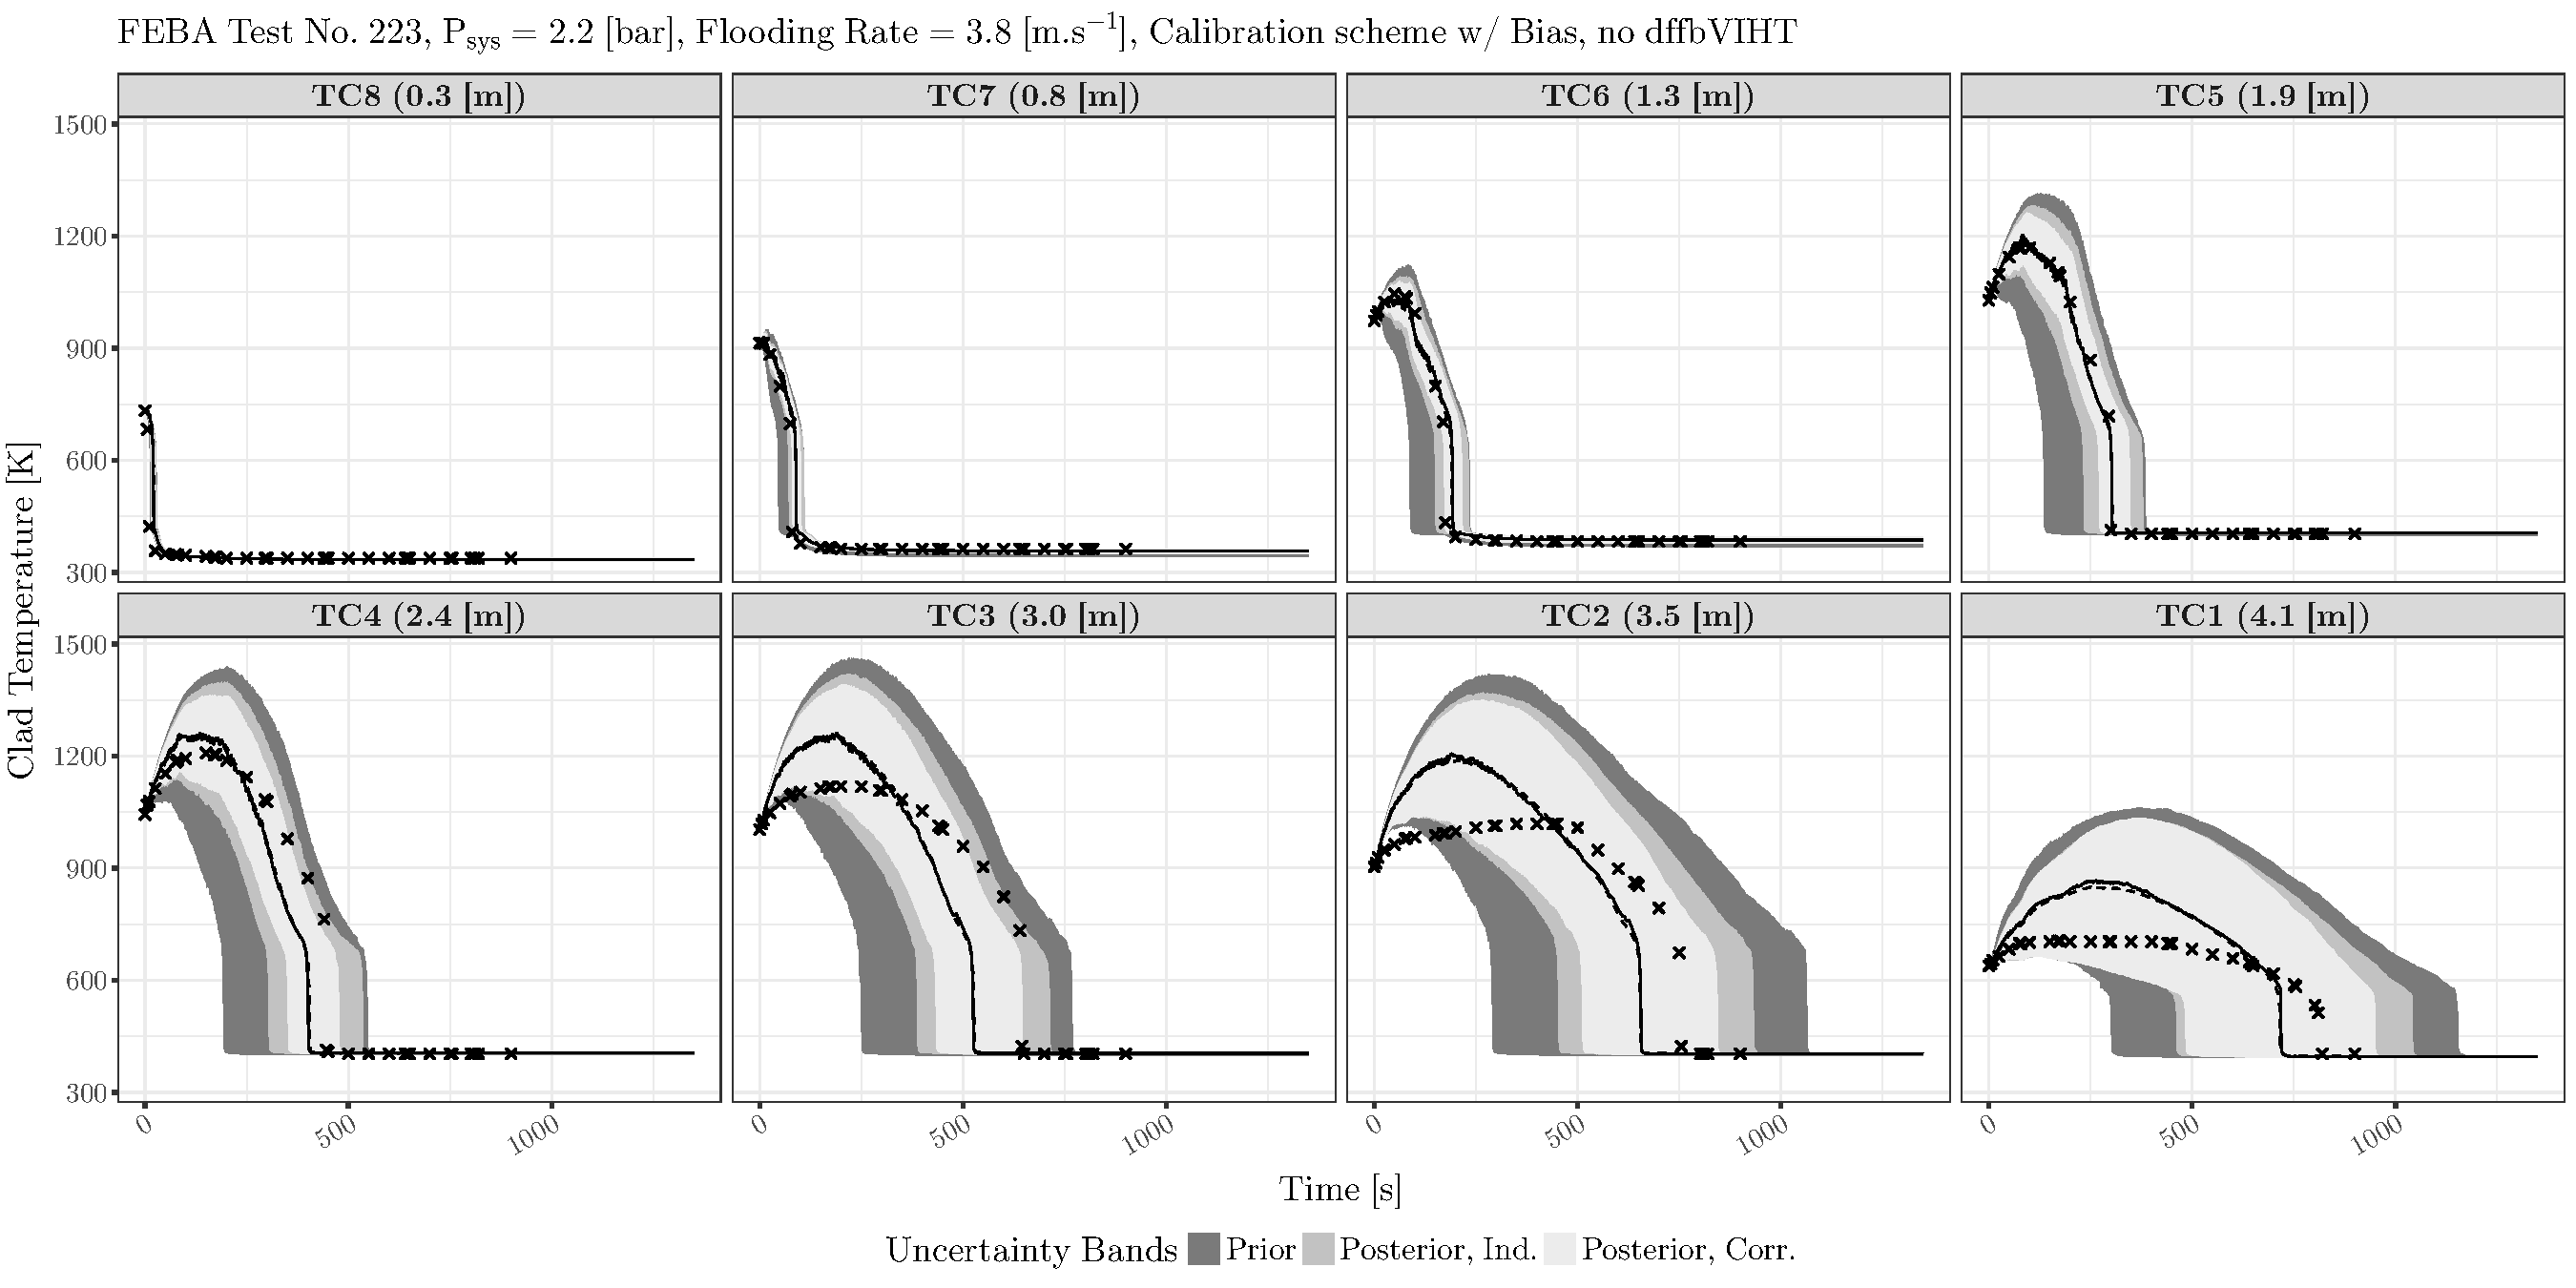
\includegraphics[width=0.90\textwidth]{../figures/chapter5/figures/plotTraceUQPosteriorAllDiscCenteredNoParam8TC223}
		\captionof{figure}[Propagation of the model parameters uncertainty on FEBA test No. $223$ for the clad temperature output ($TC$). The posterior samples are from the calibration scheme \texttt{w/ Bias, no dffbVIHT}.]{Propagation of the model parameters uncertainty on FEBA test No. $223$ for the clad temperature output ($TC$) at different axial locations. The uncertainty bands refer to the symmetric $95\%$ probabilities. Solid lines, dashed lines, and crosses indicate the simulation with the nominal parameters values, the median of the posterior, and the experimental data, respectively. The posterior samples are from the calibration with model bias term, considering all types of output, but excluding the parameter \texttt{dffbVIHT} (\texttt{w/ Bias, no dffbVIHT}).}
	\label{fig:ch5_plot_trace_uq_post_tc_223_noparam8}
\end{sidewaysfigure}
\clearpage

% FEBA Test No. 223 Posterior Uncertainty Propagation, TC, without model bias term
\clearpage
\begin{sidewaysfigure}
	\centering
	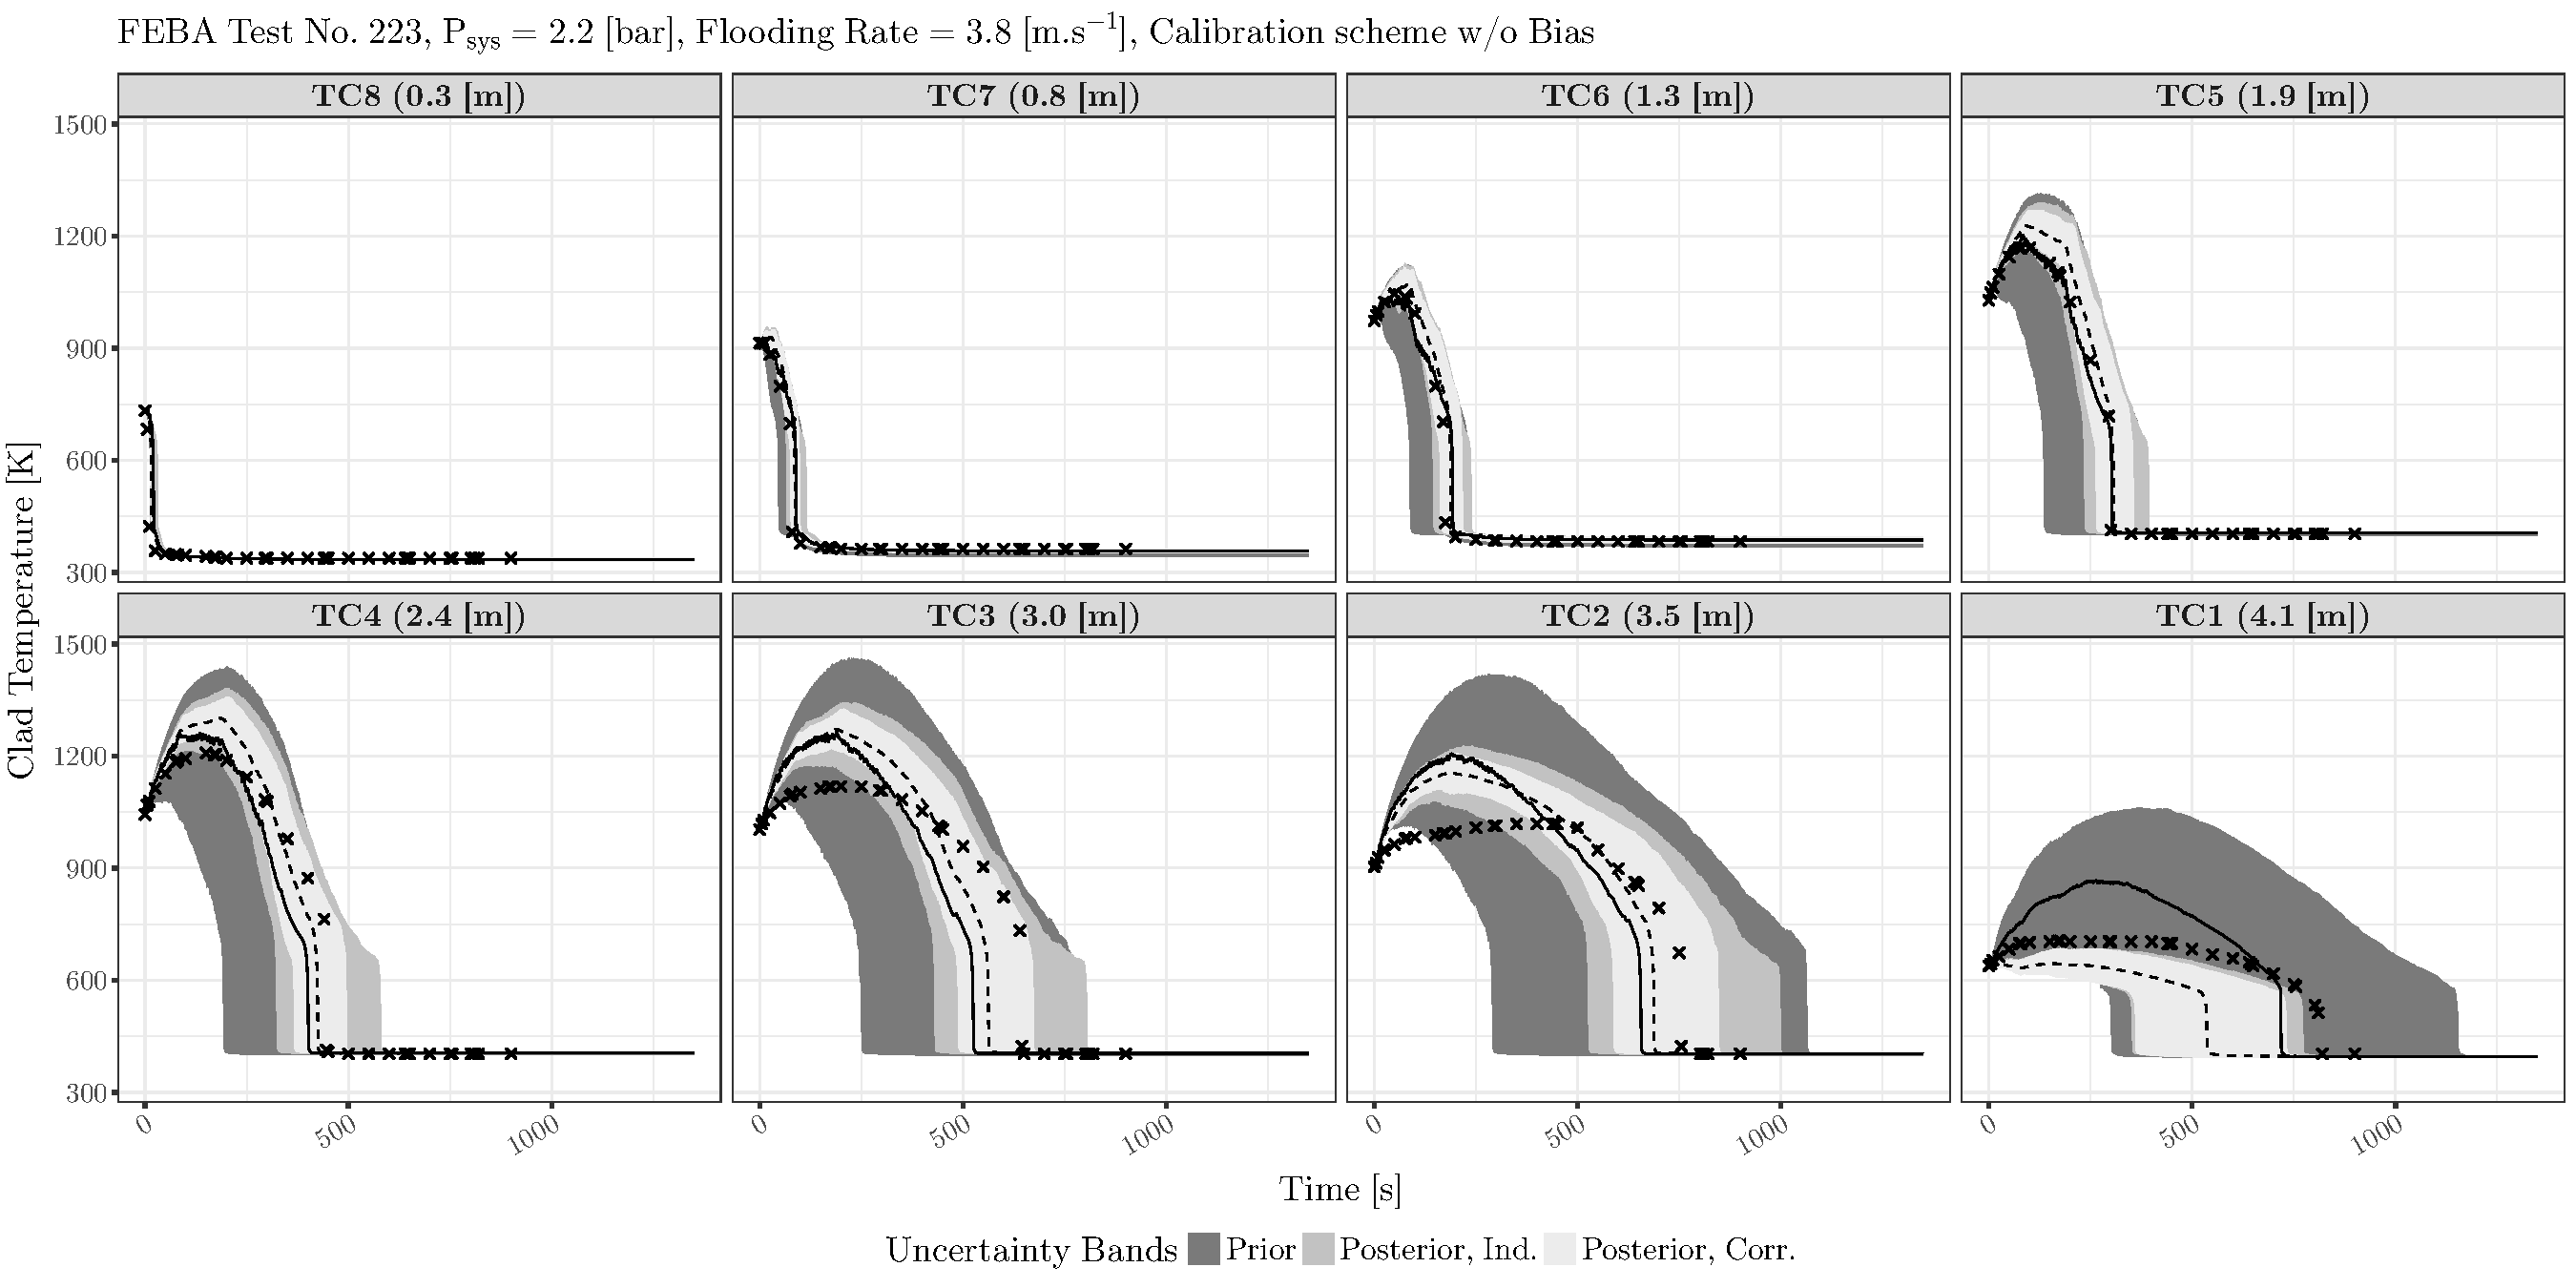
\includegraphics[width=0.90\textwidth]{../figures/chapter5/figures/plotTraceUQPosteriorAllNoDiscNoBCTC223}
		\captionof{figure}[Propagation of the model parameters uncertainty on FEBA test No. $223$ for the clad temperature output ($TC$). The posterior samples are from the calibration scheme \texttt{w/o Bias}.]{Propagation of the model parameters uncertainty on FEBA test No. $223$ for the clad temperature output ($TC$) at different axial locations. The uncertainty bands refer to the symmetric $95\%$ probabilities. Solid lines, dashed lines, and crosses indicate the simulation with the nominal parameters values, the median of the posterior, and the experimental data, respectively. The posterior samples are from the calibration without model bias term and considering all types of output (\texttt{w/o Bias}).}
	\label{fig:ch5_plot_trace_uq_post_tc_223_nodisc}
\end{sidewaysfigure}
\clearpage

%-----------------------------------------------------------------------------------------------------
\subsection{FEBA Test No. 218, clad Temperature Output (TC)}\label{app:tbl_results_uq_post_tc_218}
%-----------------------------------------------------------------------------------------------------

% FEBA Test No. 218 Posterior Uncertainty Propagation, TC, with model bias term
\rotatebox{90}{\begin{minipage}{0.85\textheight}
    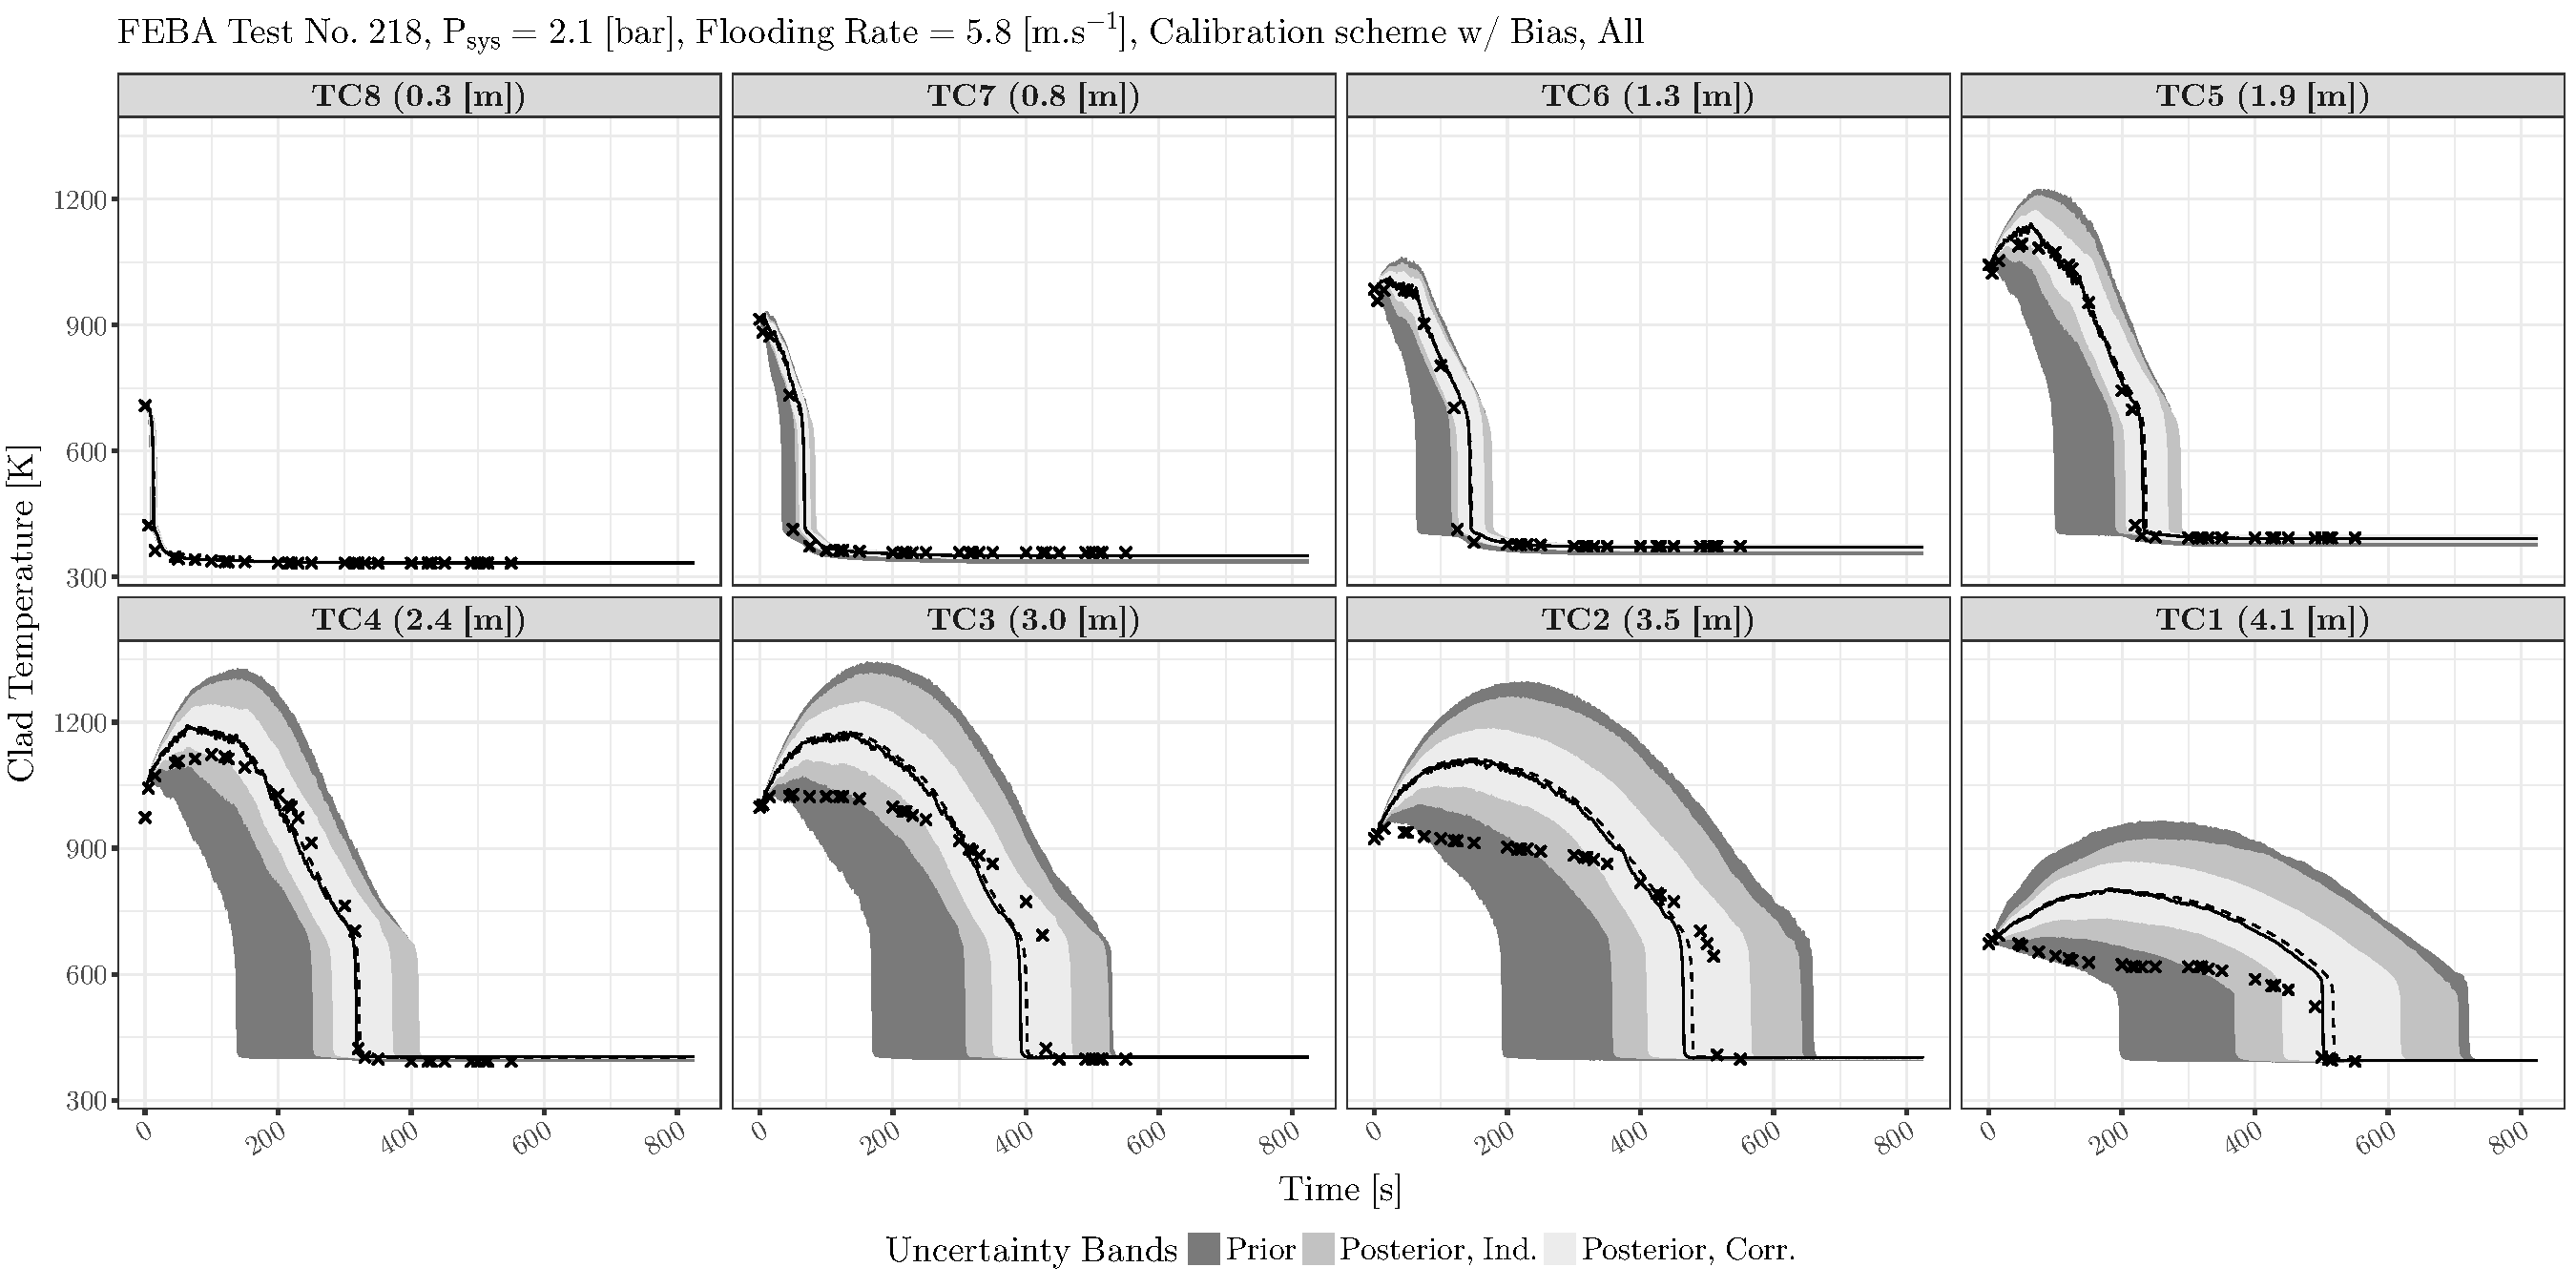
\includegraphics[width=0.95\textwidth]{../figures/chapter5/figures/plotTraceUQPosteriorAllDiscCenteredTC218}
		\captionof{figure}[Propagation of the model parameters uncertainty on FEBA test No. $218$ for the clad temperature output ($TC$). The posterior samples are from the calibration scheme \texttt{w/ Bias, All}.]{Propagation of the model parameters uncertainty on FEBA test No. $218$ for the clad temperature output ($TC$) at different axial locations. The uncertainty bands refer to the symmetric $95\%$ probabilities. Solid lines, dashed lines, and crosses indicate the simulation with the nominal parameters values, the median of the posterior, and the experimental data, respectively. The posterior samples are from the calibration with model bias term and considering all types of output (\texttt{w/ Bias, All}).}
    \label{fig:ch5_plot_trace_uq_post_tc_218_disc}
\end{minipage}}

% FEBA Test No. 218 Posterior Uncertainty Propagation, TC, without Parameter 8
\clearpage
\begin{sidewaysfigure}
	\centering
	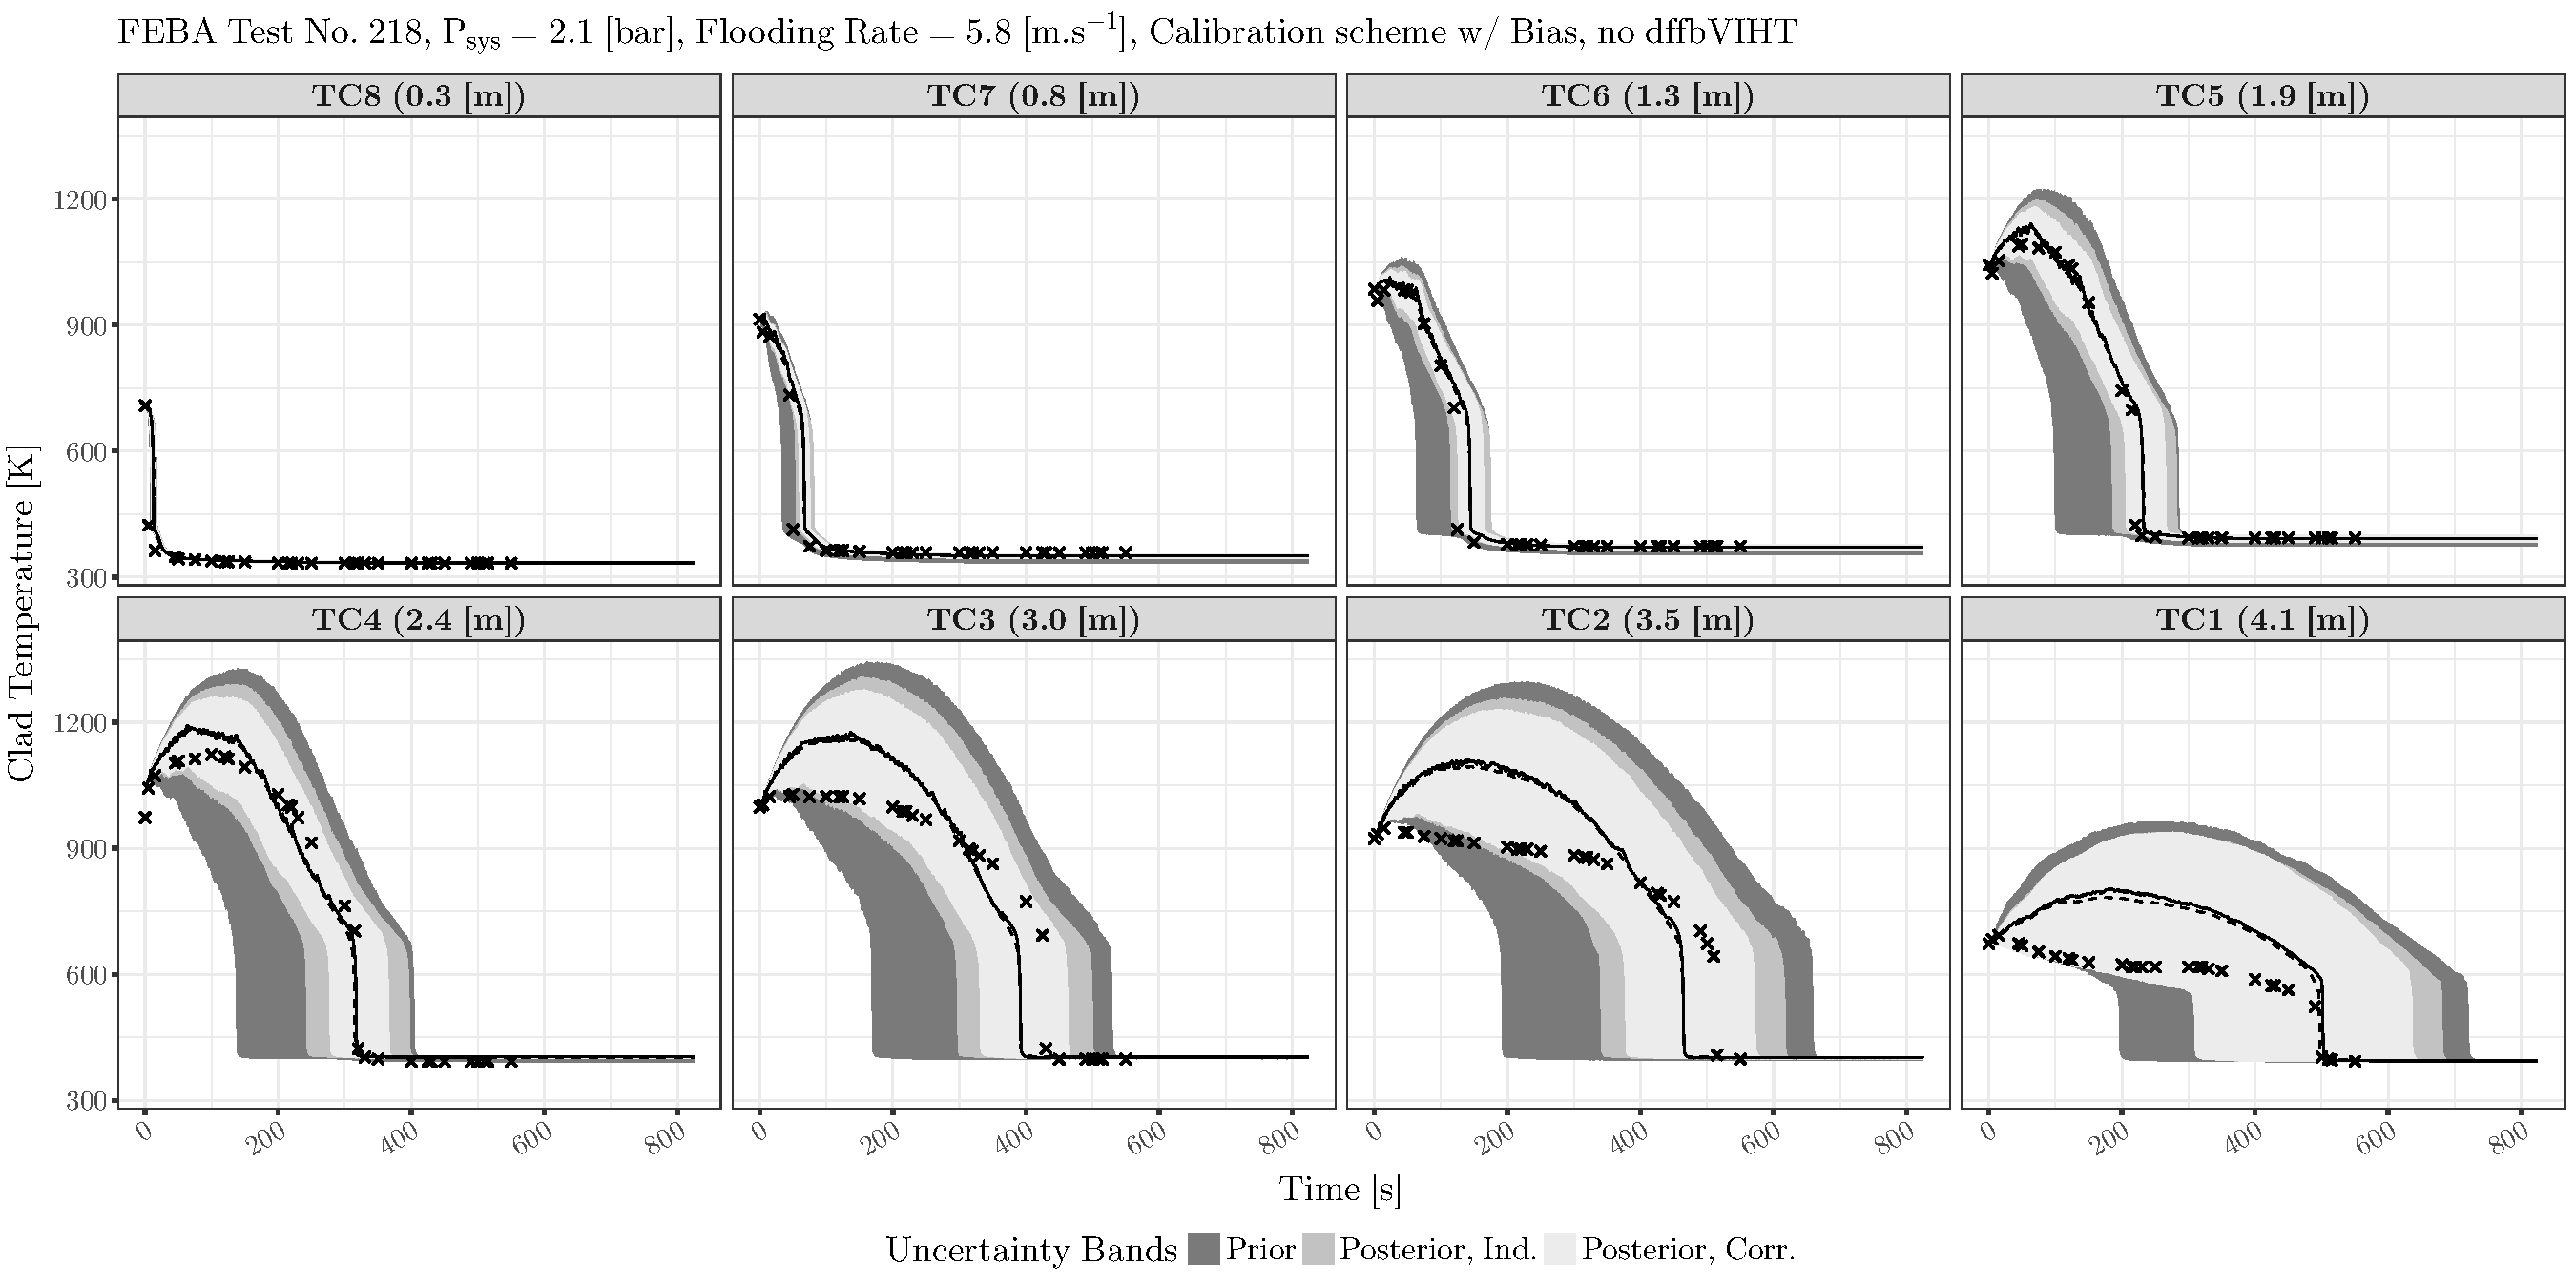
\includegraphics[width=0.90\textwidth]{../figures/chapter5/figures/plotTraceUQPosteriorAllDiscCenteredNoParam8TC218}
		\captionof{figure}[Propagation of the model parameters uncertainty on FEBA test No. $218$ for the clad temperature output ($TC$). The posterior samples are from the calibration scheme \texttt{w/ Bias, no dffbVIHT}.]{Propagation of the model parameters uncertainty on FEBA test No. $218$ for the clad temperature output ($TC$) at different axial locations. The uncertainty bands refer to the symmetric $95\%$ probabilities. Solid lines, dashed lines, and crosses indicate the simulation with the nominal parameters values, the median of the posterior, and the experimental data, respectively. The posterior samples are from the calibration with model bias term, considering all types of output, but excluding the parameter \texttt{dffbVIHT} (\texttt{w/ Bias, no dffbVIHT}).}
	\label{fig:ch5_plot_trace_uq_post_tc_218_noparam8}
\end{sidewaysfigure}
\clearpage

% FEBA Test No. 218 Posterior Uncertainty Propagation, TC, without model bias term
\clearpage
\begin{sidewaysfigure}
	\centering
	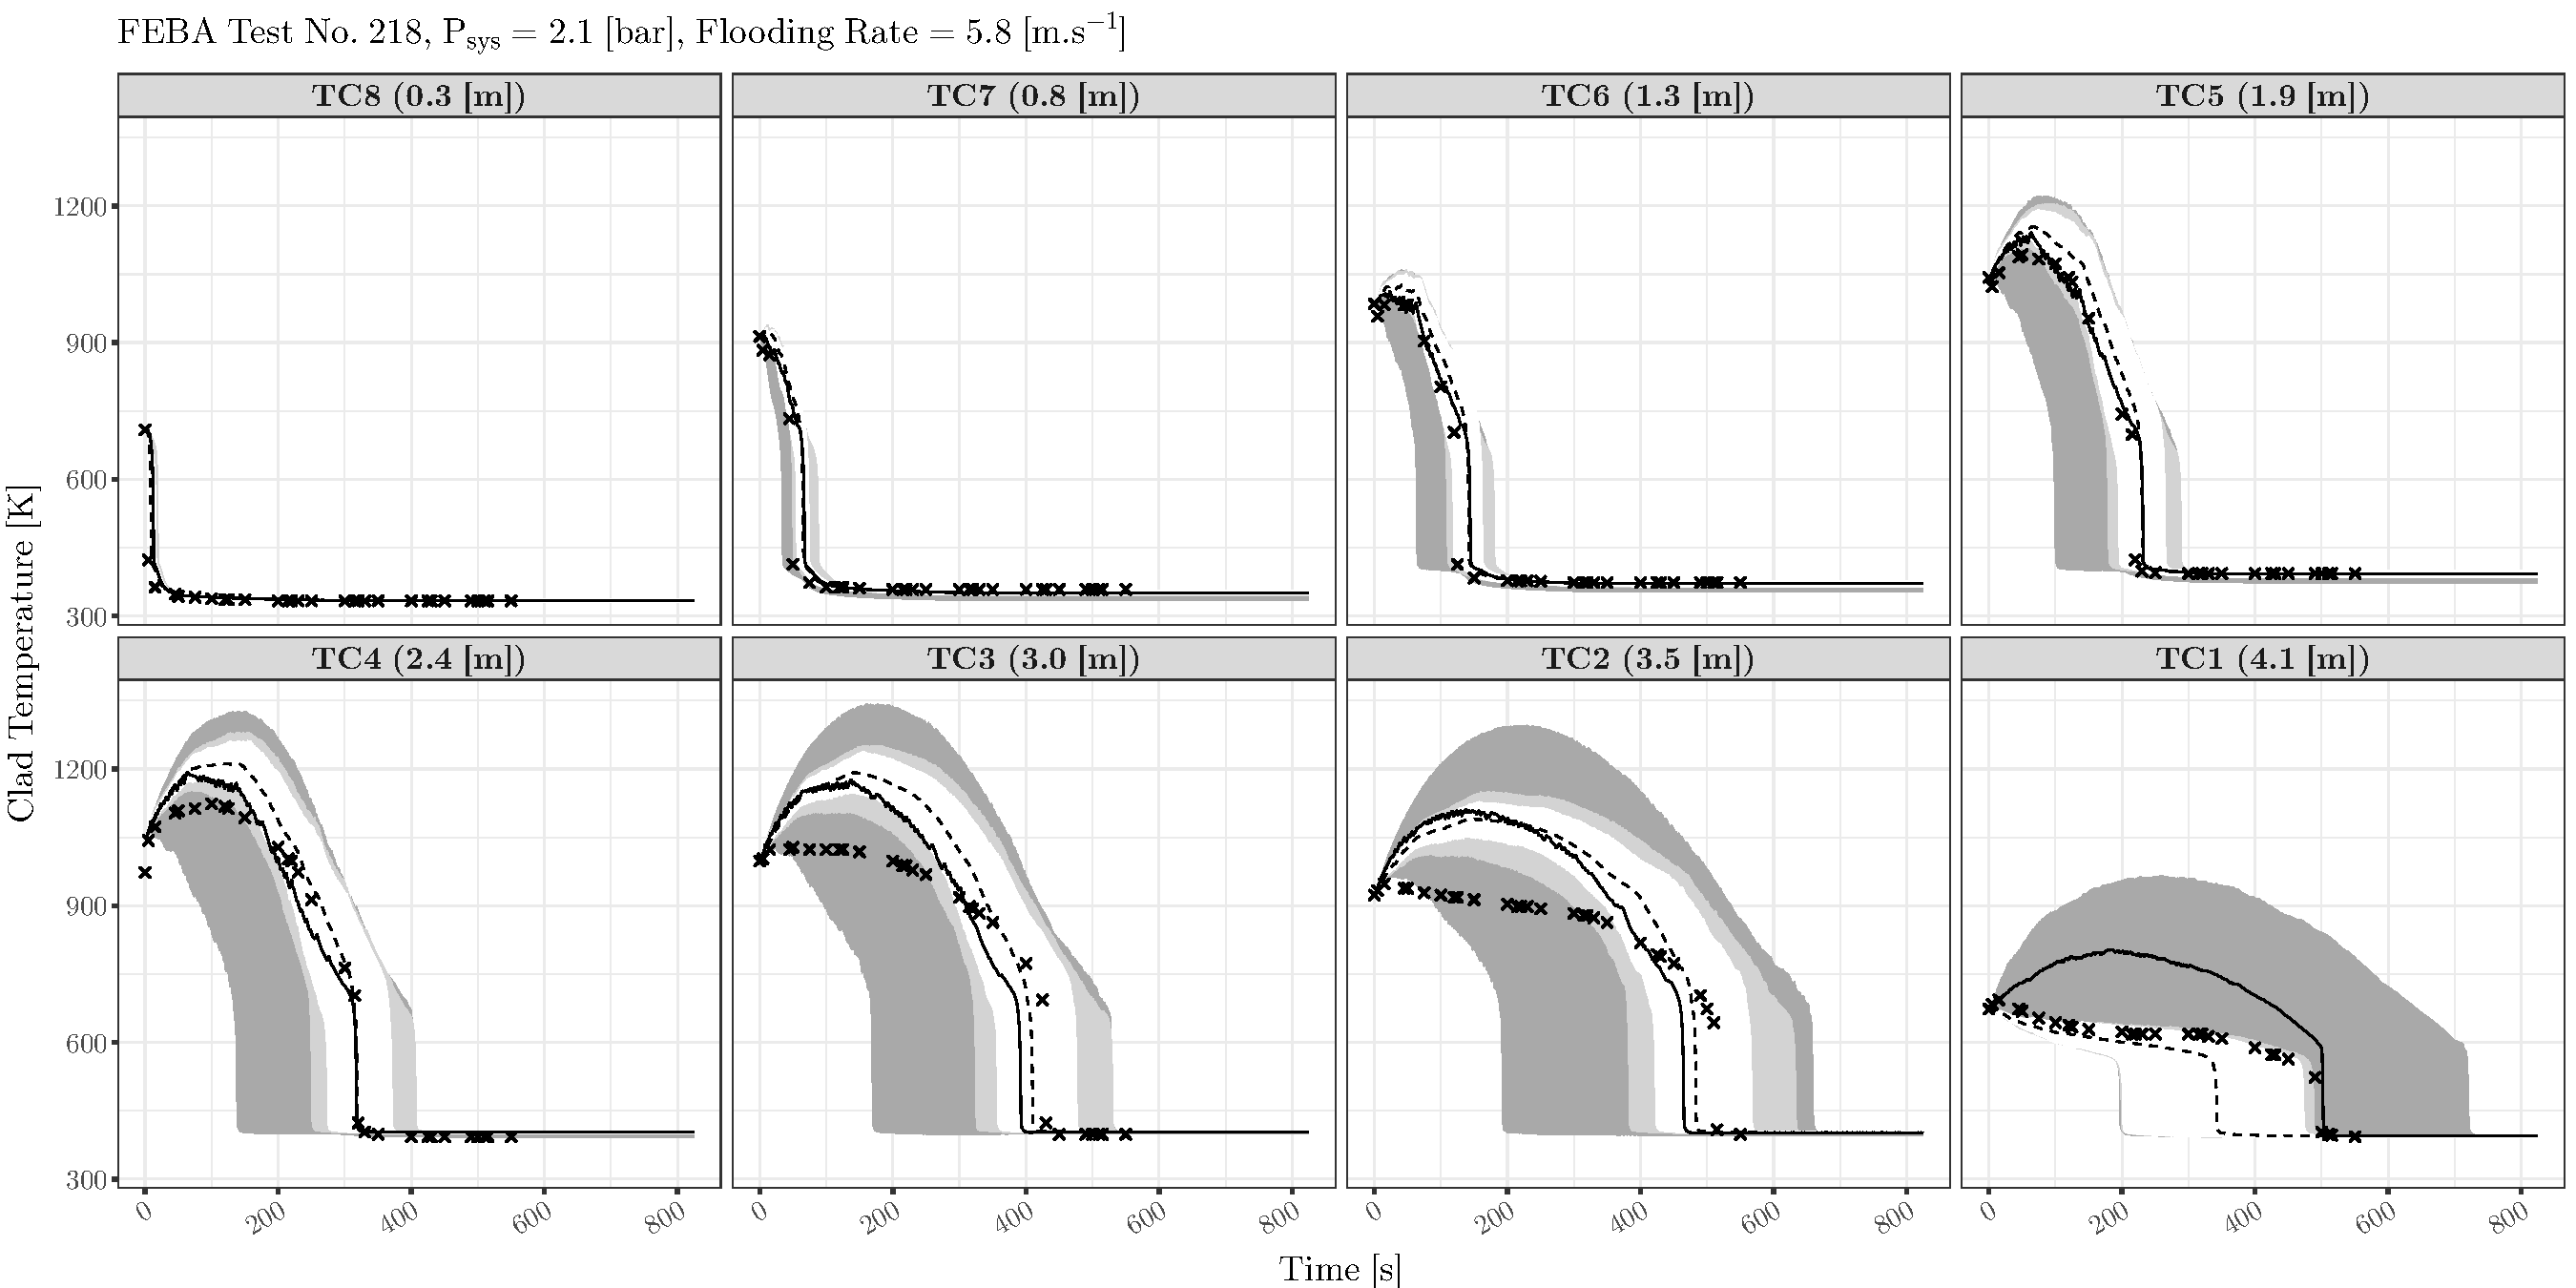
\includegraphics[width=0.90\textwidth]{../figures/chapter5/figures/plotTraceUQPosteriorAllNoDiscNoBCTC218}
		\captionof{figure}[Propagation of the model parameters uncertainty on FEBA test No. $218$ for the clad temperature output ($TC$). The posterior samples are from the calibration scheme \texttt{w/o Bias}.]{Propagation of the model parameters uncertainty on FEBA test No. $218$ for the clad temperature output ($TC$) at different axial locations. The uncertainty bands refer to the symmetric $95\%$ probabilities. Solid lines, dashed lines, and crosses indicate the simulation with the nominal parameters values, the median of the posterior, and the experimental data, respectively. The posterior samples are from the calibration without model bias term and considering all types of output (\texttt{w/o Bias}).}
	\label{fig:ch5_plot_trace_uq_post_tc_218_nodisc}
\end{sidewaysfigure}
\clearpage

%-----------------------------------------------------------------------------------------------------
\subsection{FEBA Test No. 220, clad Temperature Output (TC)}\label{app:tbl_results_uq_post_tc_220}
%-----------------------------------------------------------------------------------------------------

% FEBA Test No. 220 Posterior Uncertainty Propagation, TC, with model bias term
\rotatebox{90}{\begin{minipage}{0.85\textheight}
    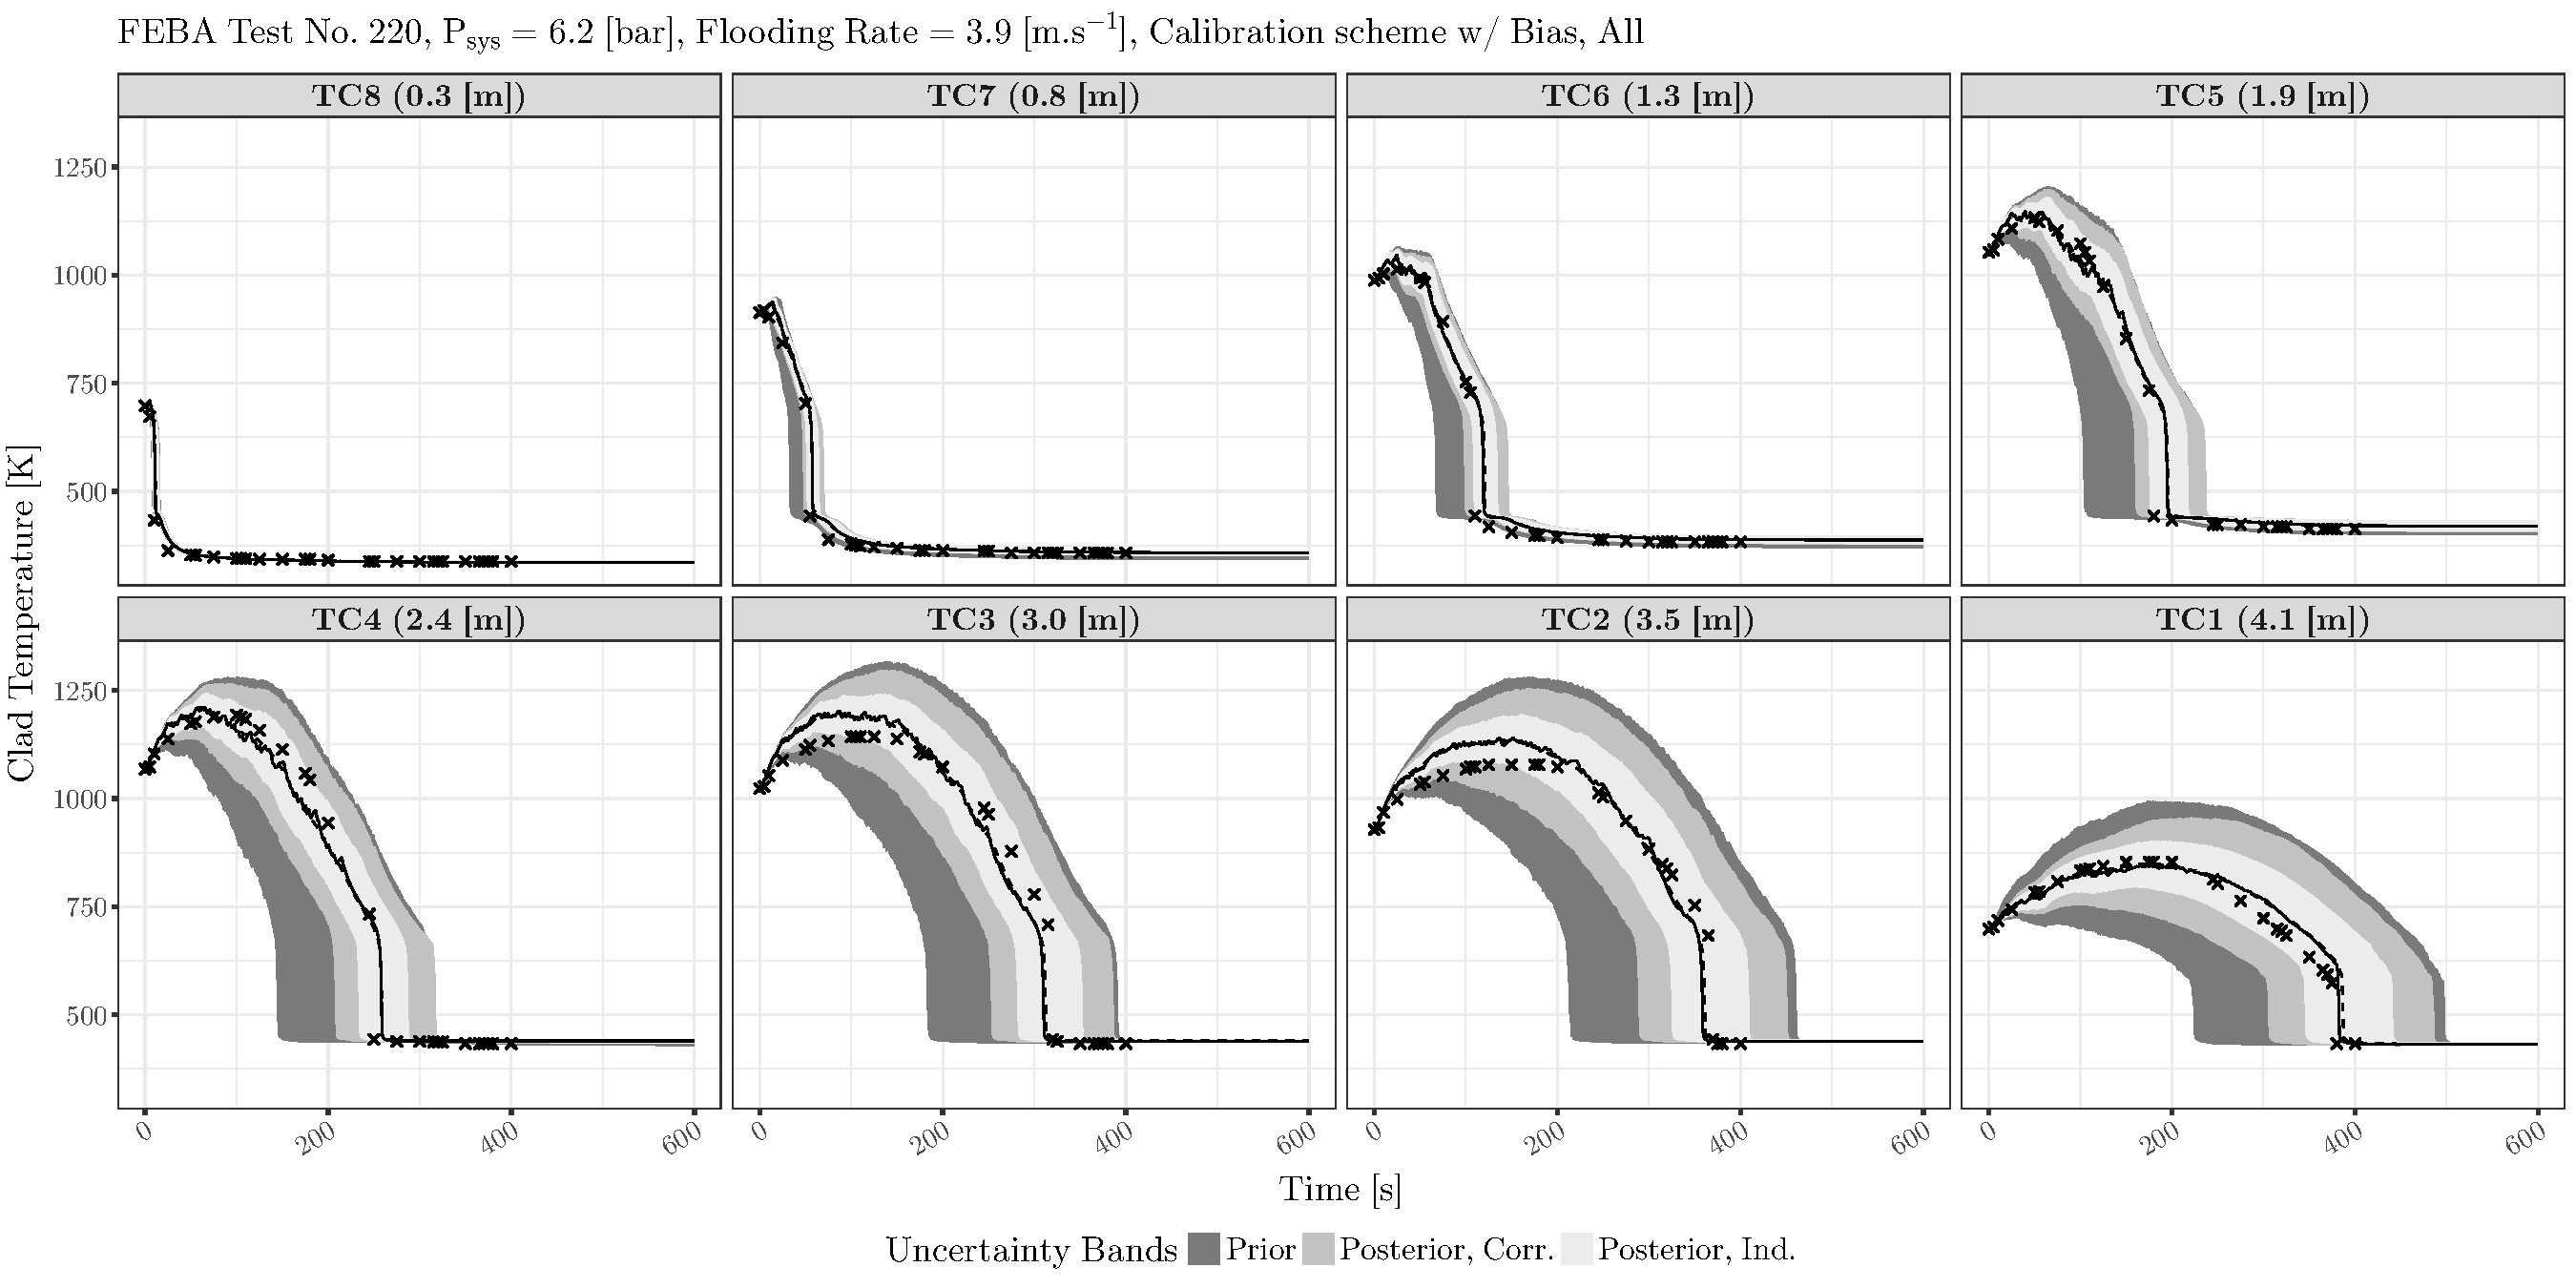
\includegraphics[width=0.95\textwidth]{../figures/chapter5/figures/plotTraceUQPosteriorAllDiscCenteredTC220}
		\captionof{figure}[Propagation of the model parameters uncertainty on FEBA test No. $220$ for the clad temperature output ($TC$). The posterior samples are from the calibration scheme \texttt{w/ Bias, All}.]{Propagation of the model parameters uncertainty on FEBA test No. $220$ for the clad temperature output ($TC$) at different axial locations. The uncertainty bands refer to the symmetric $95\%$ probabilities. Solid lines, dashed lines, and crosses indicate the simulation with the nominal parameters values, the median of the posterior, and the experimental data, respectively. The posterior samples are from the calibration with model bias term and considering all types of output (\texttt{w/ Bias, All}).}
    \label{fig:ch5_plot_trace_uq_post_tc_220_disc}
\end{minipage}}

% FEBA Test No. 220 Posterior Uncertainty Propagation, TC, without Parameter 8
\clearpage
\begin{sidewaysfigure}
	\centering
	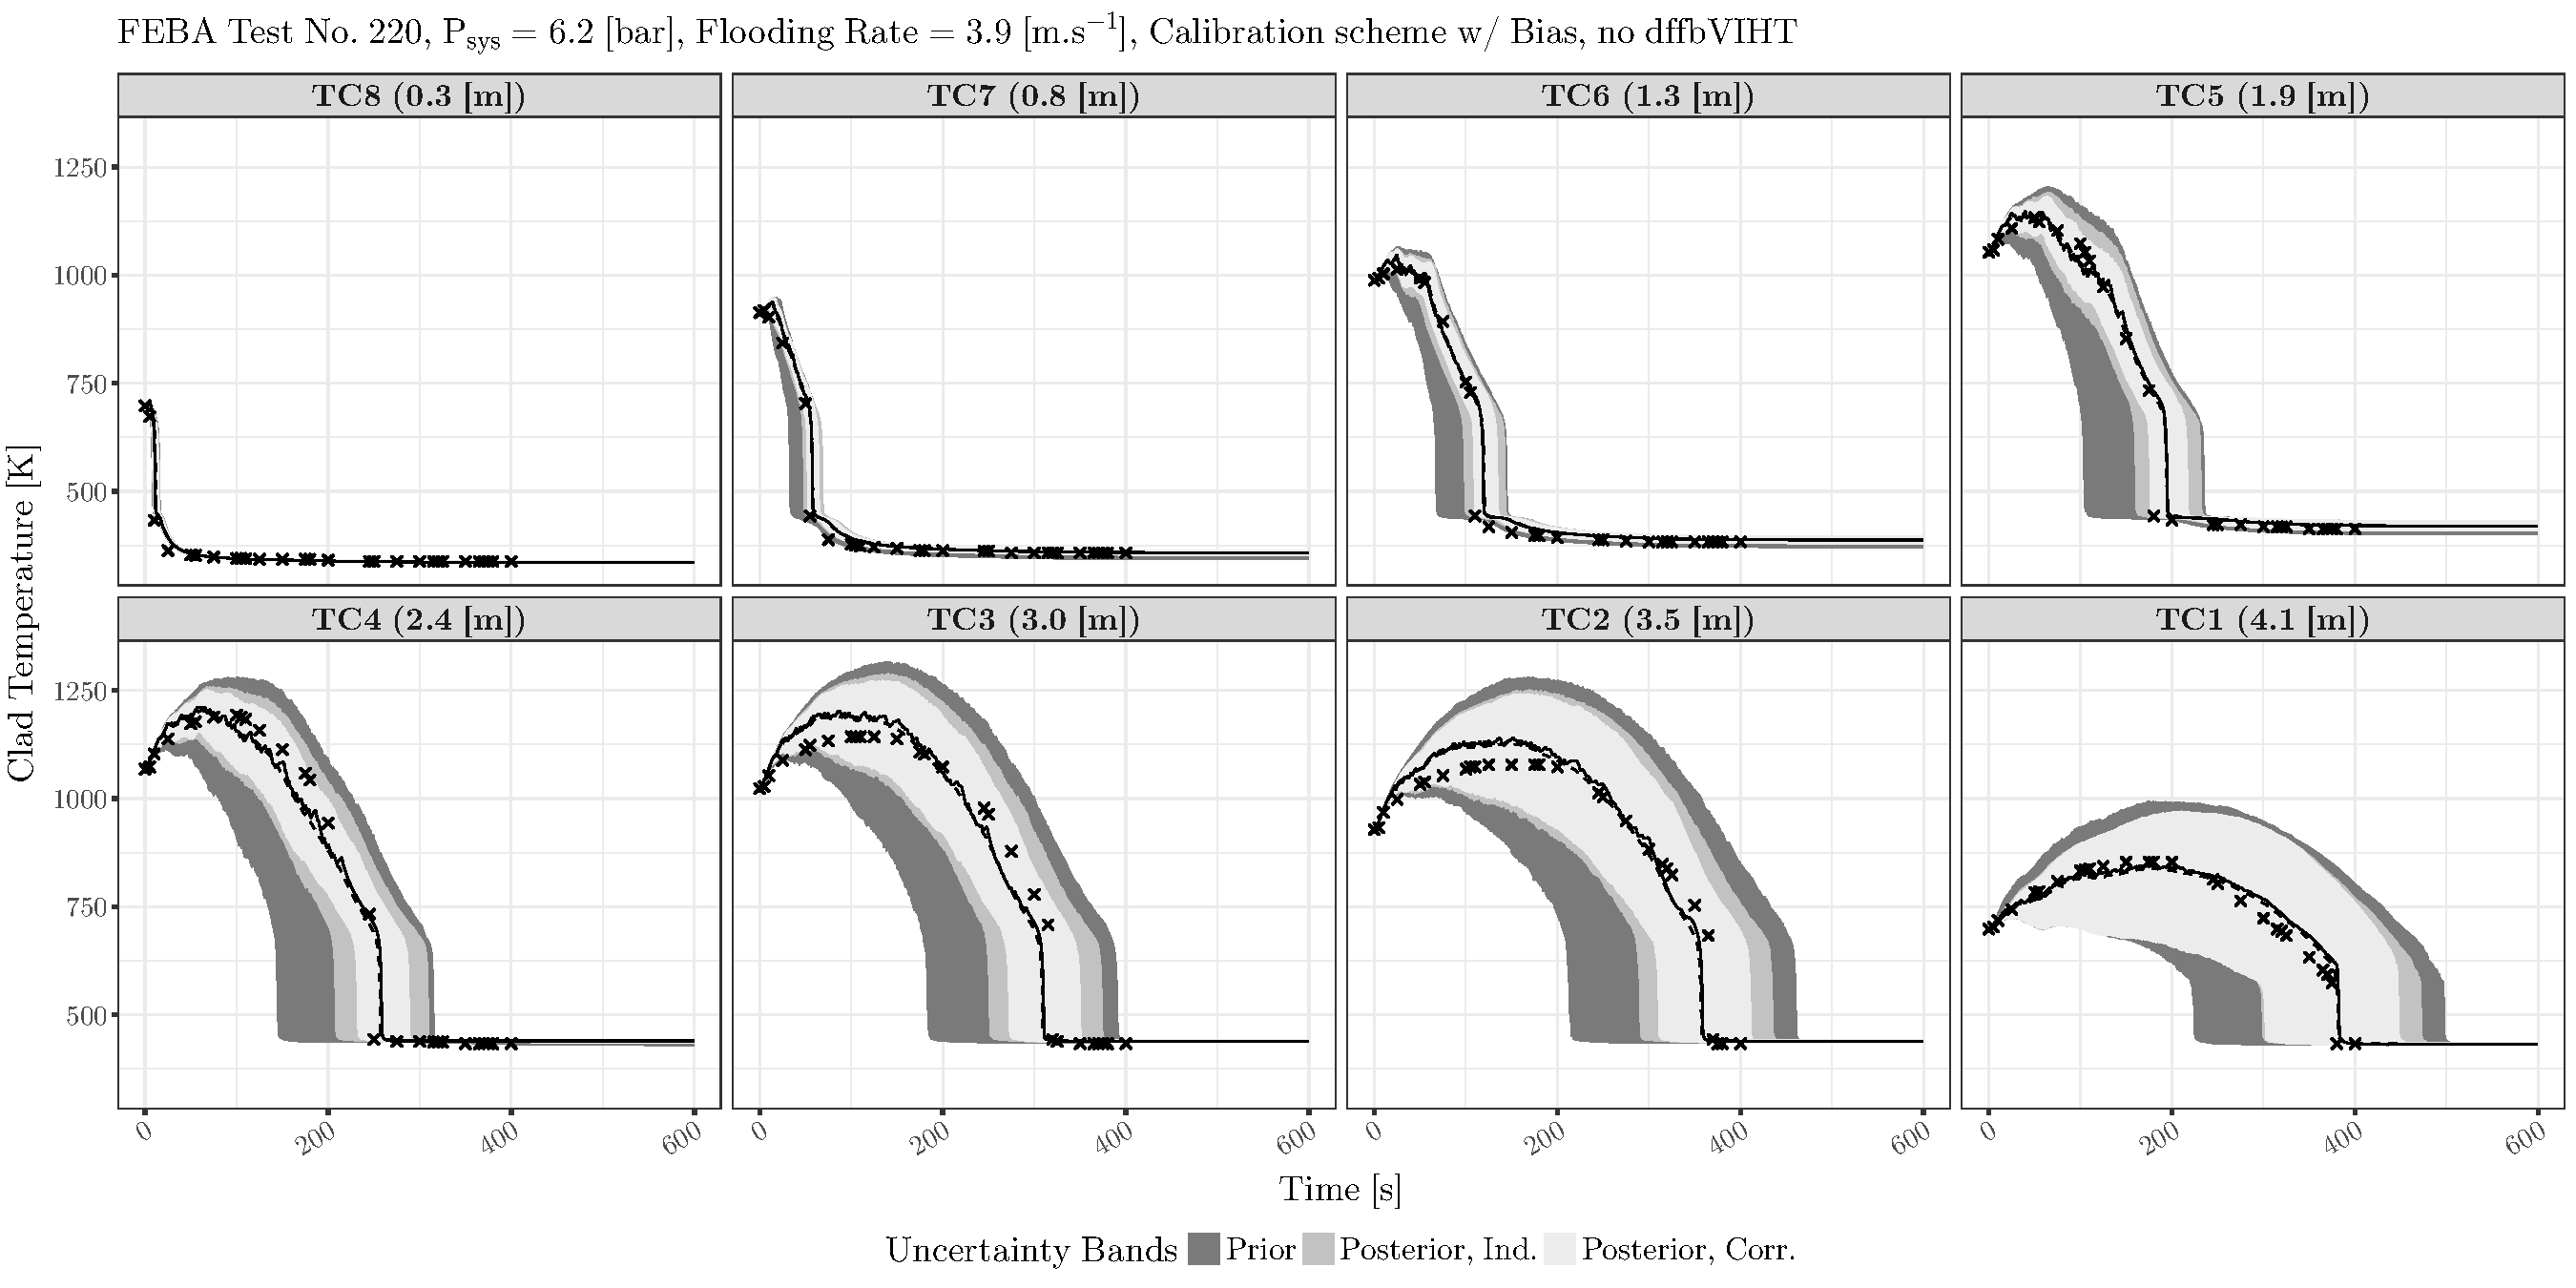
\includegraphics[width=0.90\textwidth]{../figures/chapter5/figures/plotTraceUQPosteriorAllDiscCenteredNoParam8TC220}
		\captionof{figure}[Propagation of the model parameters uncertainty on FEBA test No. $220$ for the clad temperature output ($TC$). The posterior samples are from the calibration scheme \texttt{w/ Bias, no dffbVIHT}.]{Propagation of the model parameters uncertainty on FEBA test No. $220$ for the clad temperature output ($TC$) at different axial locations. The uncertainty bands refer to the symmetric $95\%$ probabilities. Solid lines, dashed lines, and crosses indicate the simulation with the nominal parameters values, the median of the posterior, and the experimental data, respectively. The posterior samples are from the calibration with model bias term, considering all types of output, but excluding the parameter \texttt{dffbVIHT} (\texttt{w/ Bias, no dffbVIHT}).}
	\label{fig:ch5_plot_trace_uq_post_tc_220_noparam8}
\end{sidewaysfigure}
\clearpage

% FEBA Test No. 220 Posterior Uncertainty Propagation, TC, without model bias term
\clearpage
\begin{sidewaysfigure}
	\centering
	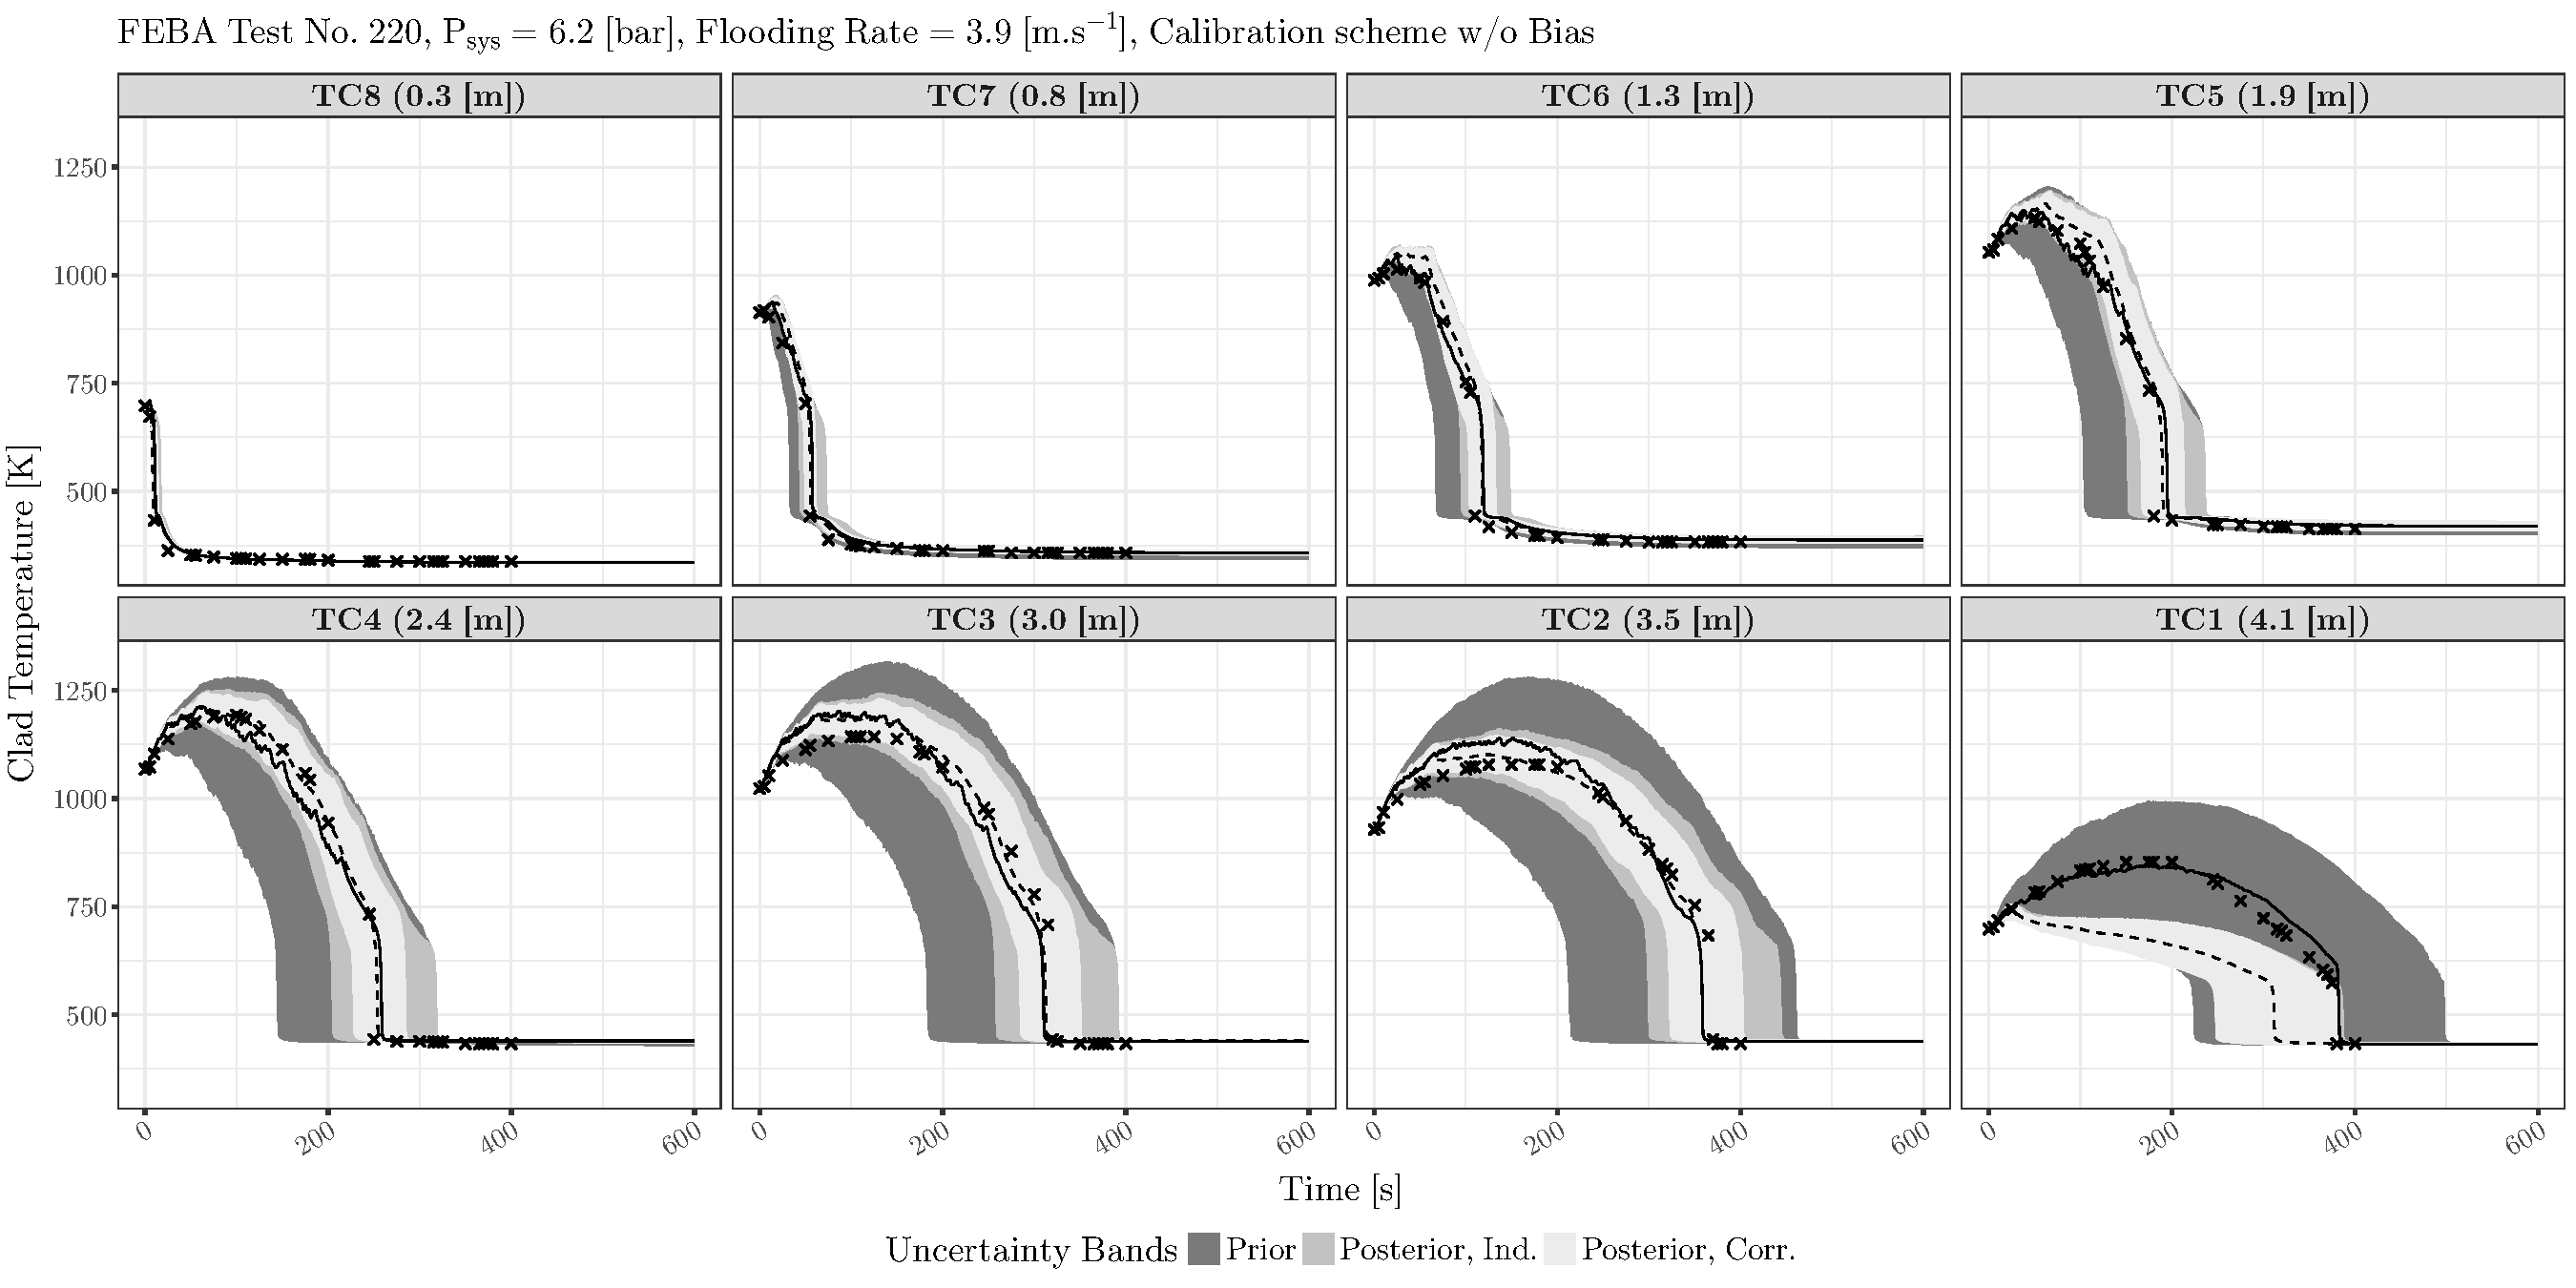
\includegraphics[width=0.90\textwidth]{../figures/chapter5/figures/plotTraceUQPosteriorAllNoDiscNoBCTC220}
		\captionof{figure}[Propagation of the model parameters uncertainty on FEBA test No. $220$ for the clad temperature output ($TC$). The posterior samples are from the calibration scheme \texttt{w/o Bias}.]{Propagation of the model parameters uncertainty on FEBA test No. $220$ for the clad temperature output ($TC$) at different axial locations. The uncertainty bands refer to the symmetric $95\%$ probabilities. Solid lines, dashed lines, and crosses indicate the simulation with the nominal parameters values, the median of the posterior, and the experimental data, respectively. The posterior samples are from the calibration without model bias term and considering all types of output (\texttt{w/o Bias}).}
	\label{fig:ch5_plot_trace_uq_post_tc_220_nodisc}
\end{sidewaysfigure}
\clearpage

%-----------------------------------------------------------------------------------------------------
\subsection{FEBA Test No. 222, clad Temperature Output (TC)}\label{app:tbl_results_uq_post_tc_222}
%-----------------------------------------------------------------------------------------------------

% FEBA Test No. 222 Posterior Uncertainty Propagation, TC, with model bias term
\rotatebox{90}{\begin{minipage}{0.85\textheight}
    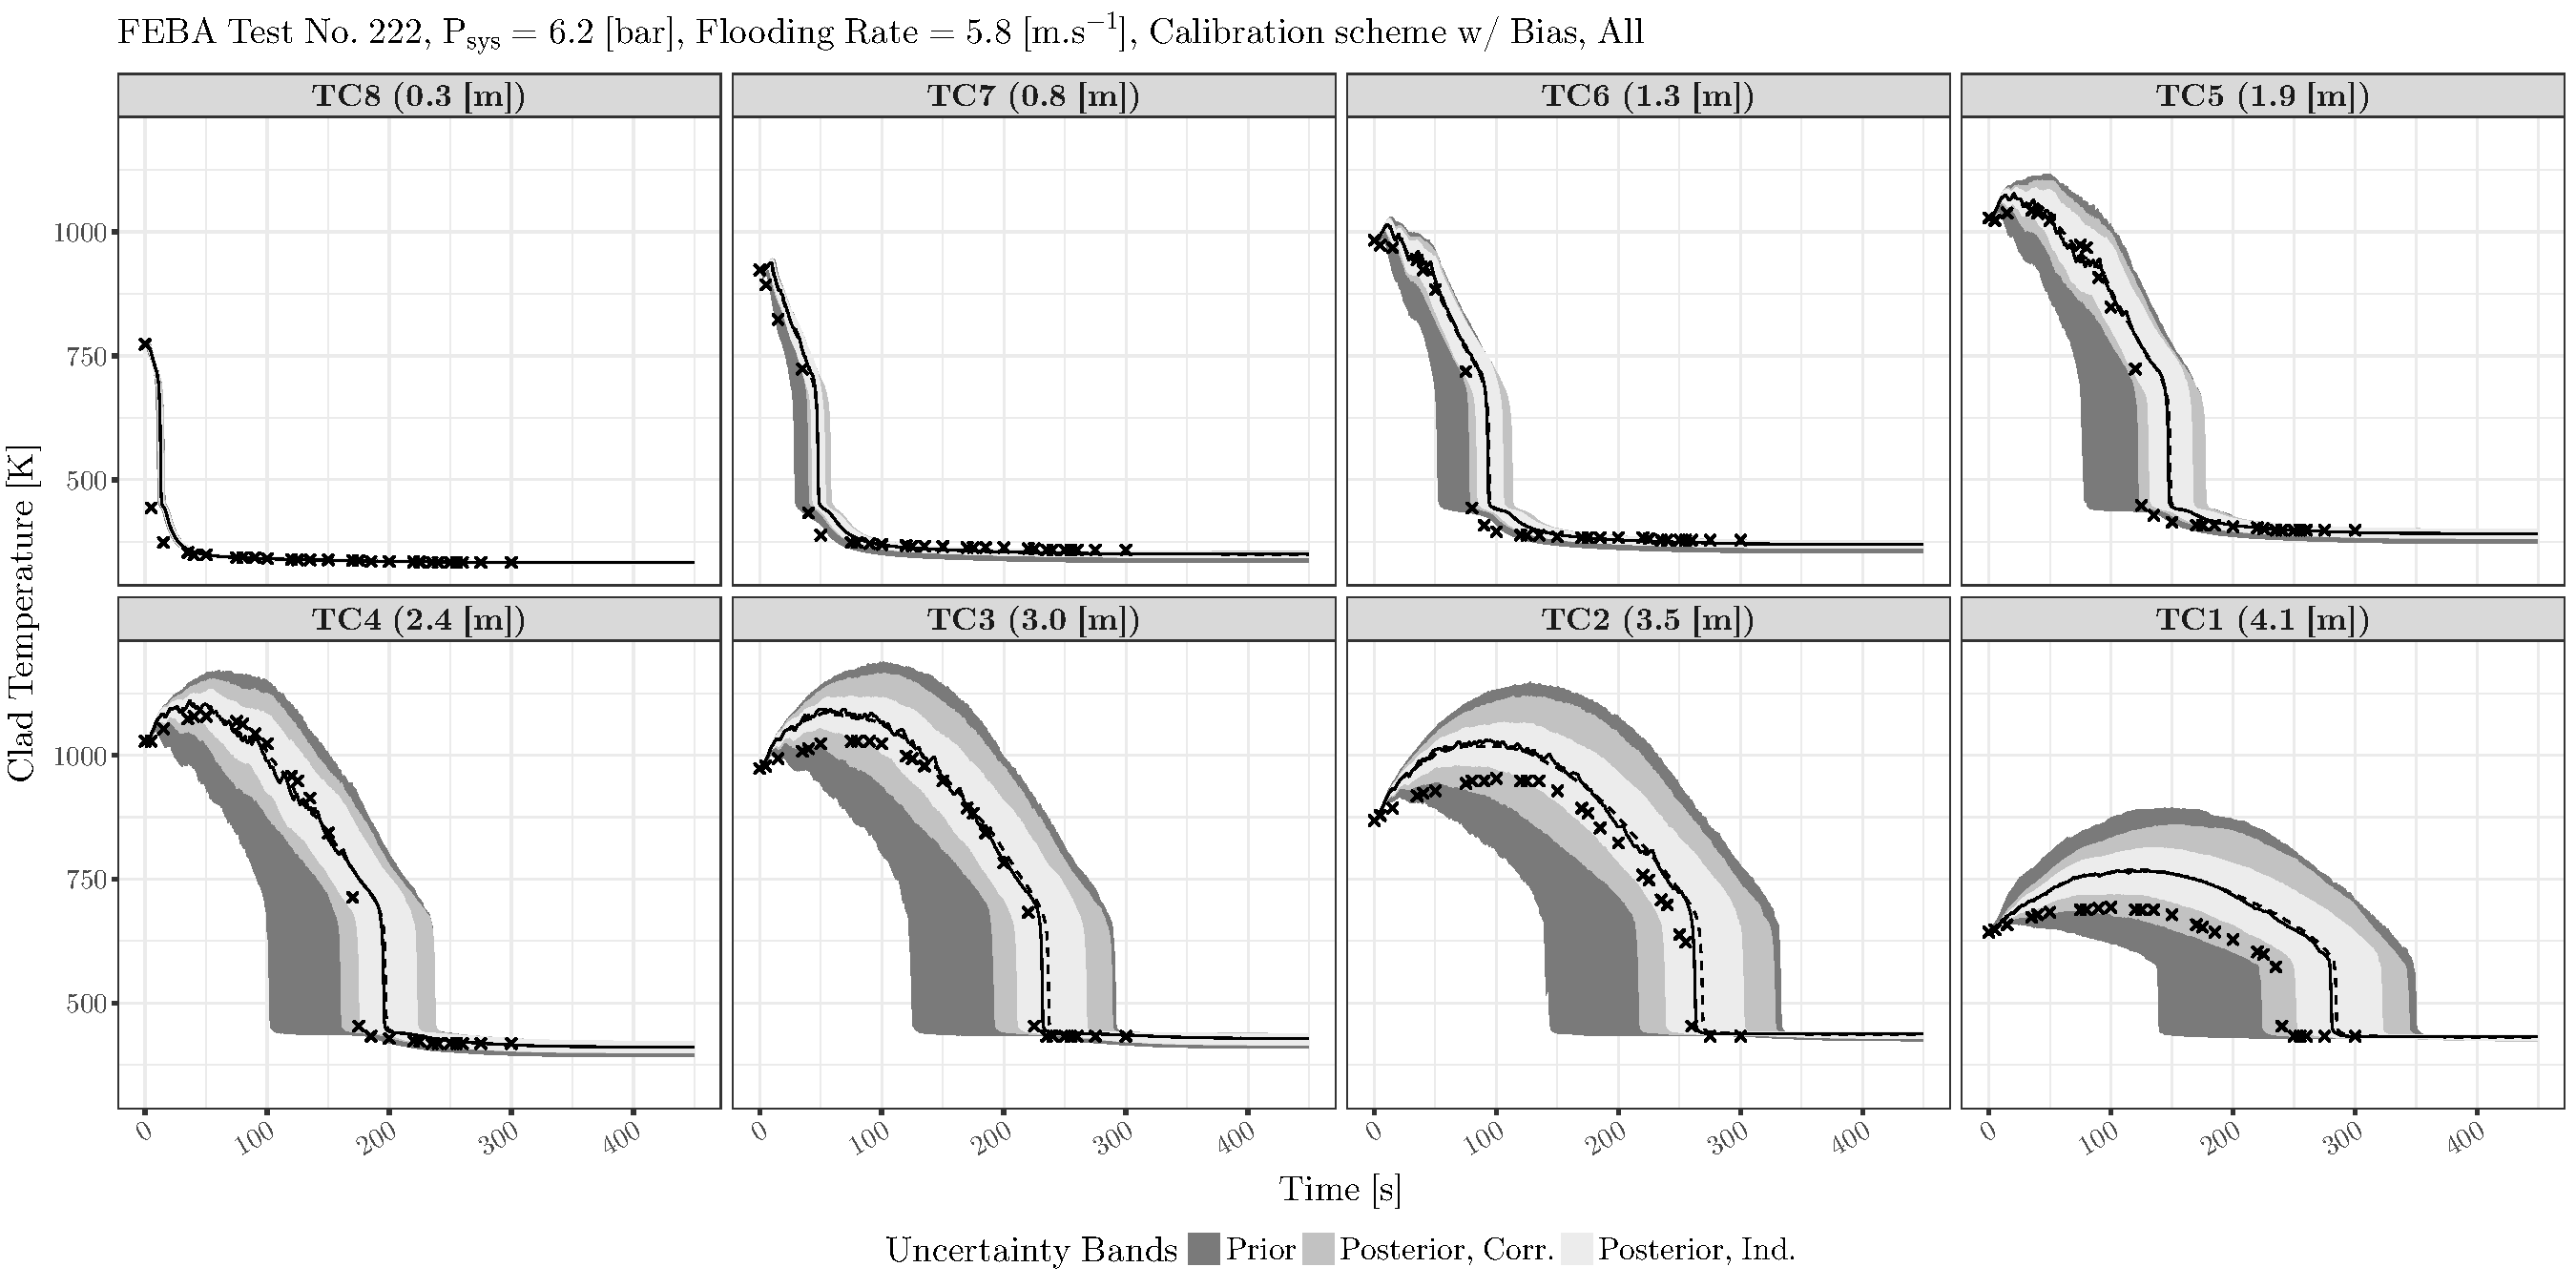
\includegraphics[width=0.95\textwidth]{../figures/chapter5/figures/plotTraceUQPosteriorAllDiscCenteredTC222}
		\captionof{figure}[Propagation of the model parameters uncertainty on FEBA test No. $222$ for the clad temperature output ($TC$). The posterior samples are from the calibration scheme \texttt{w/ Bias, All}.]{Propagation of the model parameters uncertainty on FEBA test No. $222$ for the clad temperature output ($TC$) at different axial locations. The uncertainty bands refer to the symmetric $95\%$ probabilities. Solid lines, dashed lines, and crosses indicate the simulation with the nominal parameters values, the median of the posterior, and the experimental data, respectively. The posterior samples are from the calibration with model bias term and considering all types of output (\texttt{w/ Bias, All}).}
    \label{fig:ch5_plot_trace_uq_post_tc_222_disc}
\end{minipage}}

% FEBA Test No. 222 Posterior Uncertainty Propagation, TC, without Parameter 8
\clearpage
\begin{sidewaysfigure}
	\centering
	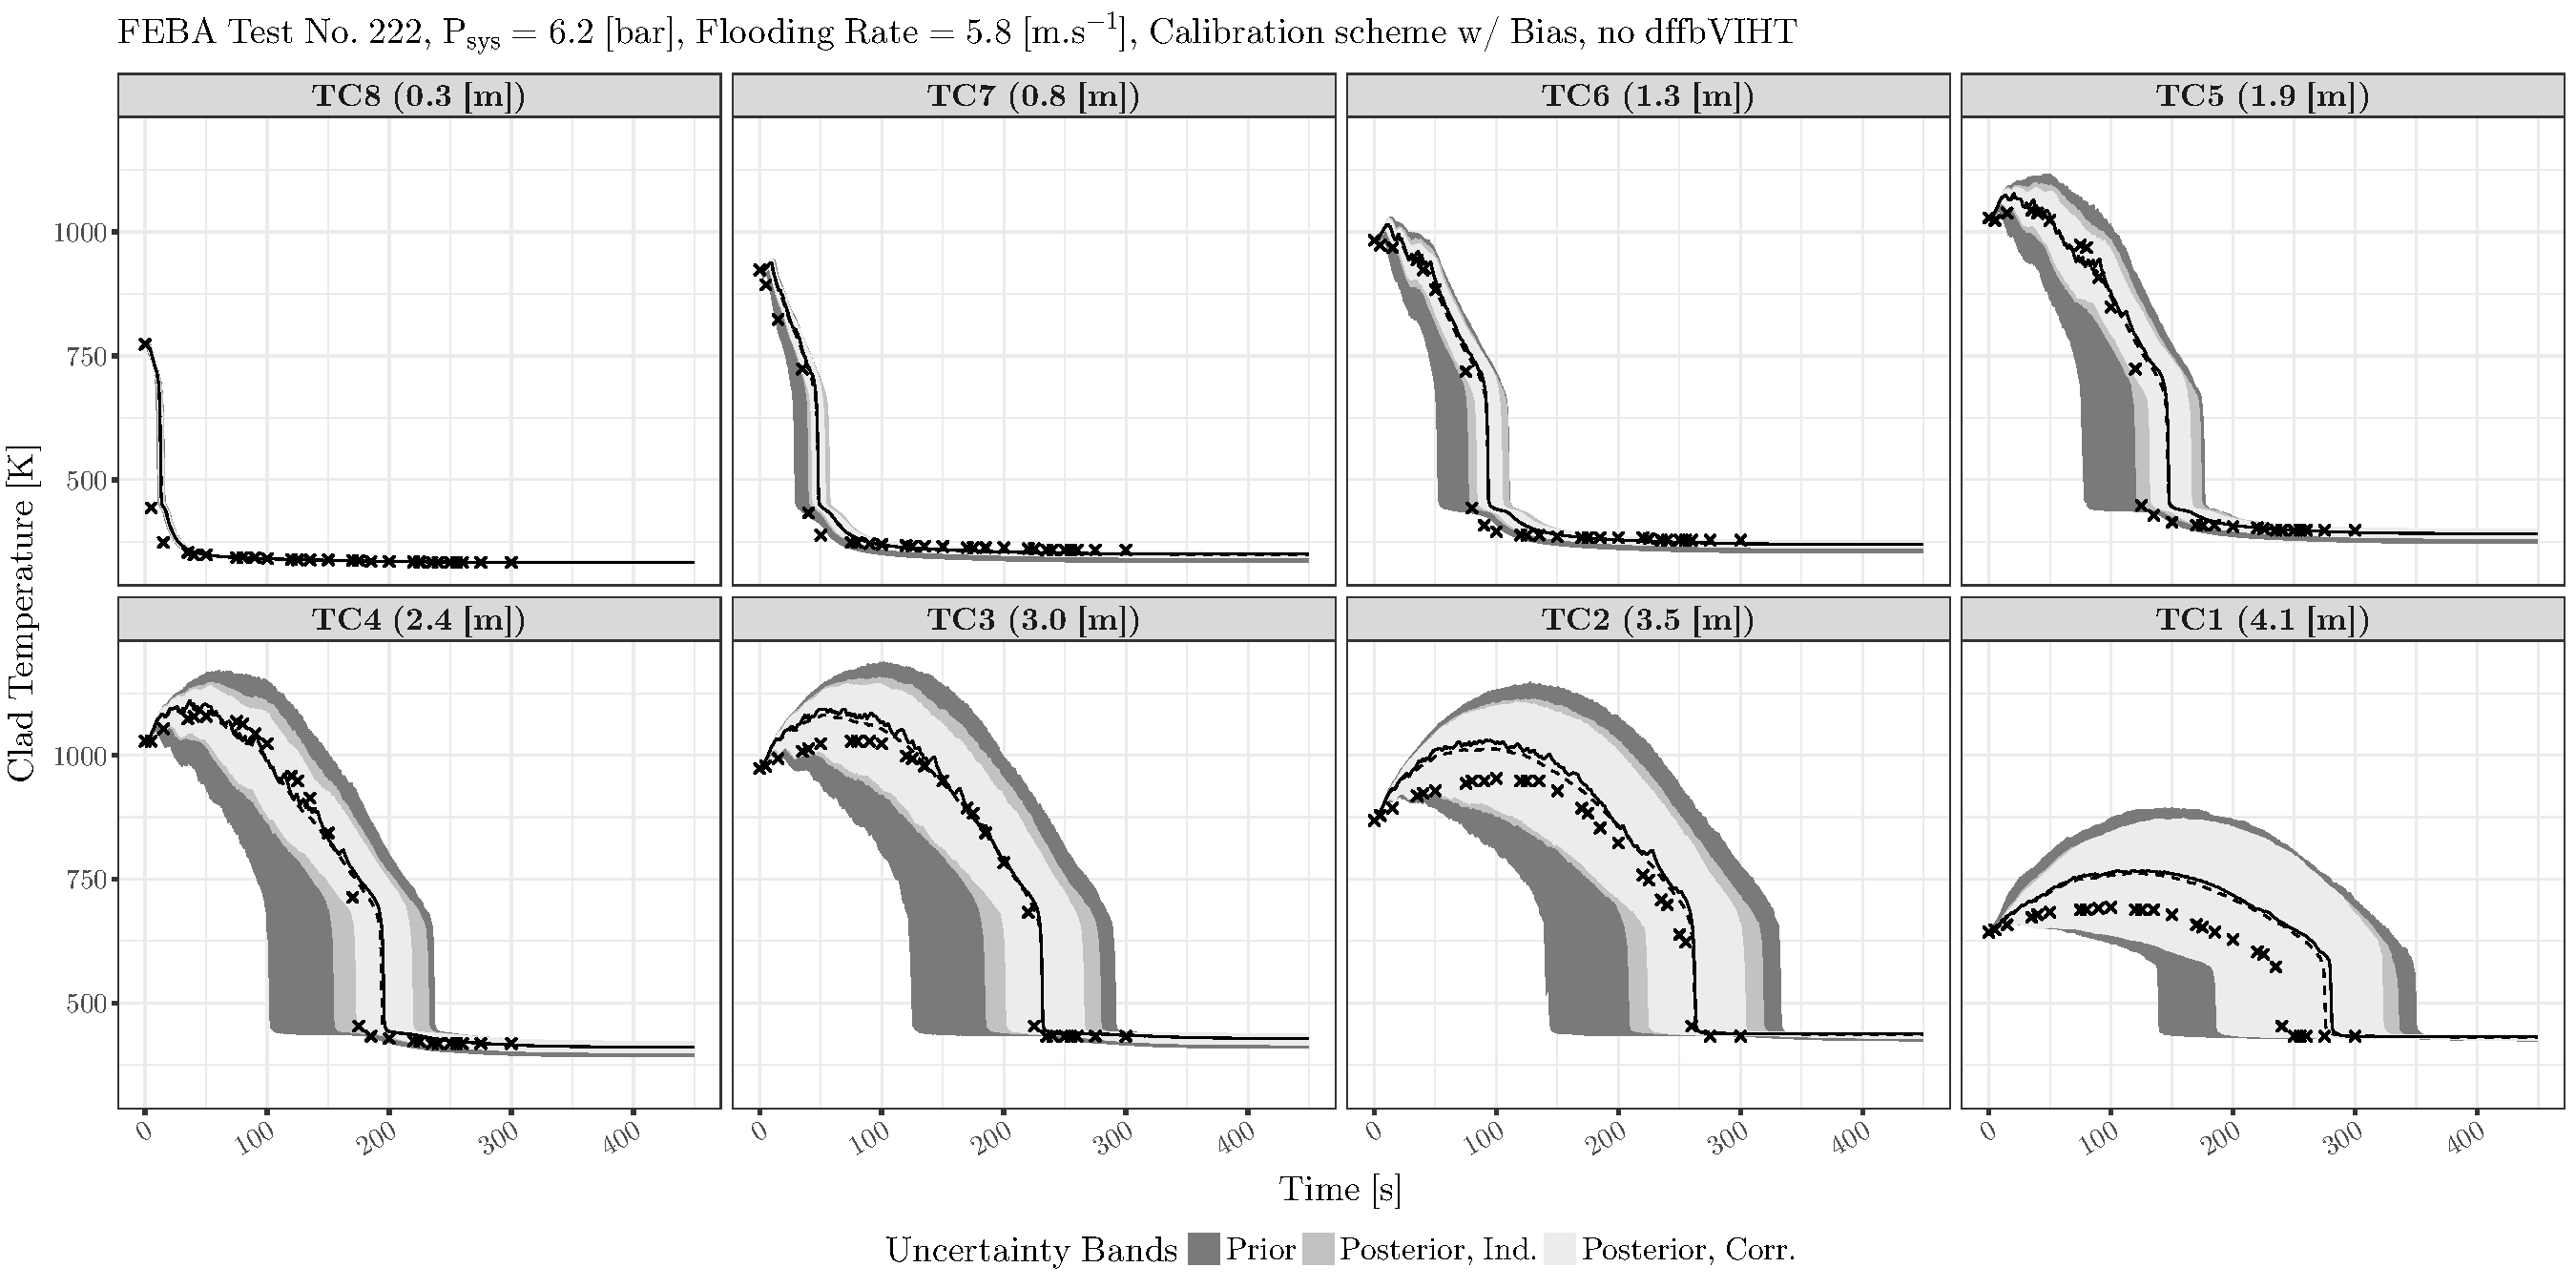
\includegraphics[width=0.90\textwidth]{../figures/chapter5/figures/plotTraceUQPosteriorAllDiscCenteredNoParam8TC222}
		\captionof{figure}[Propagation of the model parameters uncertainty on FEBA test No. $222$ for the clad temperature output ($TC$). The posterior samples are from the calibration scheme \texttt{w/ Bias, no dffbVIHT}.]{Propagation of the model parameters uncertainty on FEBA test No. $222$ for the clad temperature output ($TC$) at different axial locations. The uncertainty bands refer to the symmetric $95\%$ probabilities. Solid lines, dashed lines, and crosses indicate the simulation with the nominal parameters values, the median of the posterior, and the experimental data, respectively. The posterior samples are from the calibration with model bias term, considering all types of output, but excluding the parameter \texttt{dffbVIHT} (\texttt{w/ Bias, no dffbVIHT}).}
	\label{fig:ch5_plot_trace_uq_post_tc_222_noparam8}
\end{sidewaysfigure}
\clearpage

% FEBA Test No. 222 Posterior Uncertainty Propagation, TC, without model bias term
\clearpage
\begin{sidewaysfigure}
	\centering
	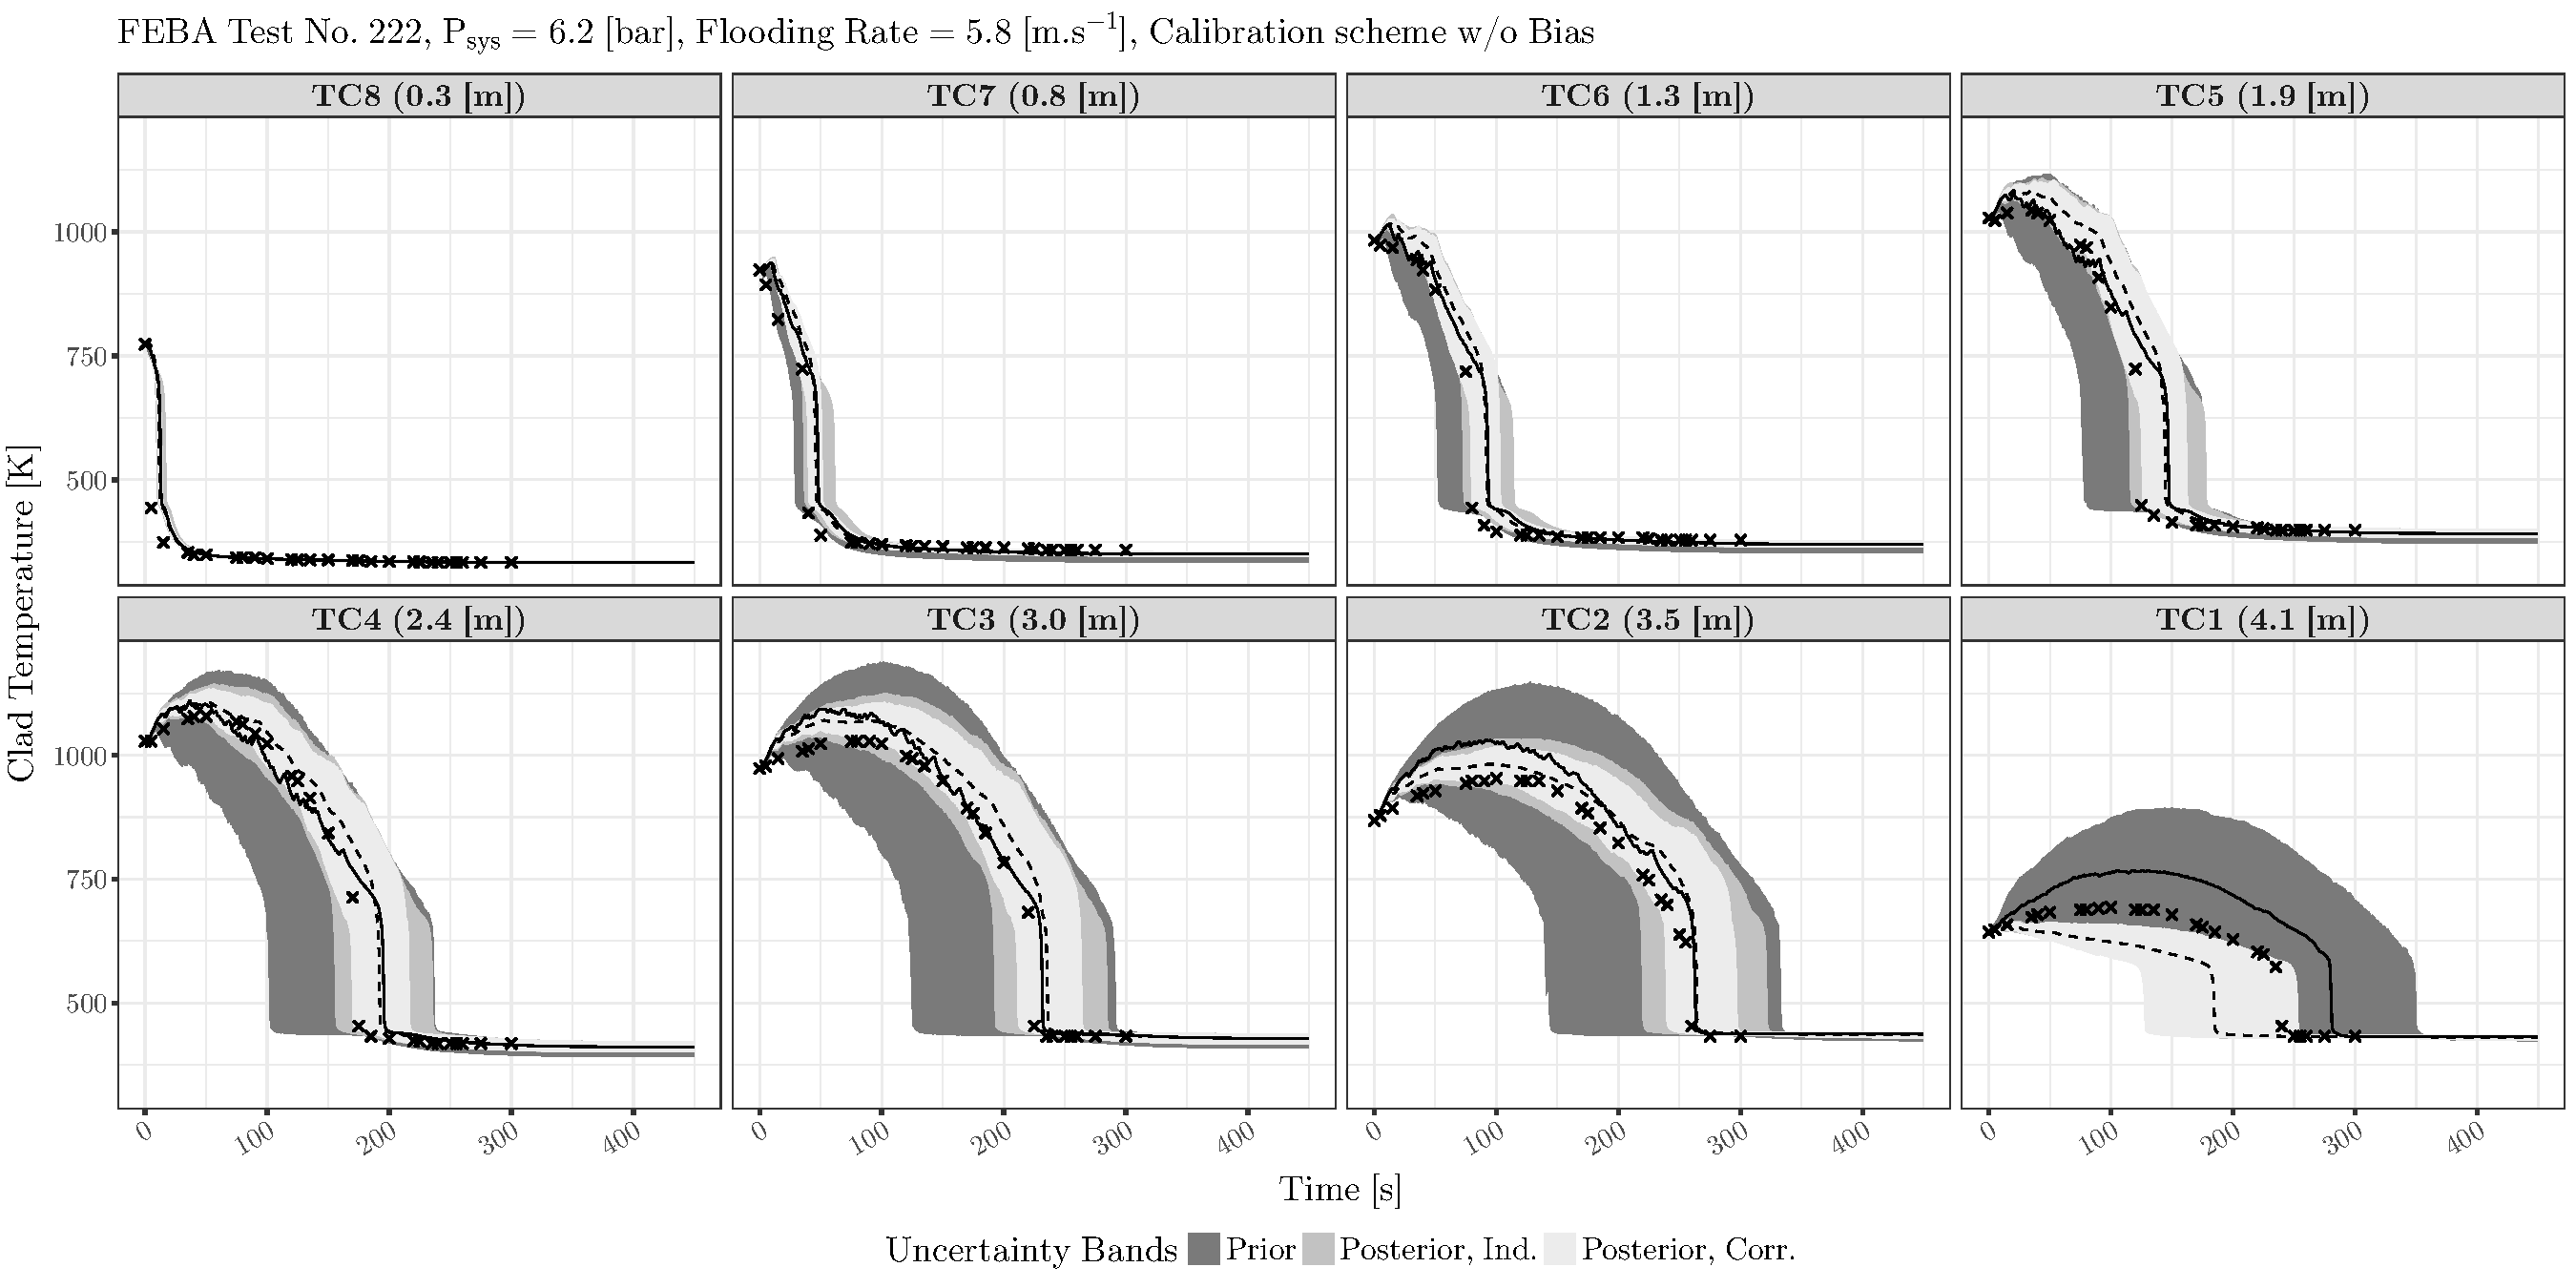
\includegraphics[width=0.90\textwidth]{../figures/chapter5/figures/plotTraceUQPosteriorAllNoDiscNoBCTC222}
		\captionof{figure}[Propagation of the model parameters uncertainty on FEBA test No. $222$ for the clad temperature output ($TC$). The posterior samples are from the calibration scheme \texttt{w/o Bias}.]{Propagation of the model parameters uncertainty on FEBA test No. $222$ for the clad temperature output ($TC$) at different axial locations. The uncertainty bands refer to the symmetric $95\%$ probabilities. Solid lines, dashed lines, and crosses indicate the simulation with the nominal parameters values, the median of the posterior, and the experimental data, respectively. The posterior samples are from the calibration without model bias term and considering all types of output (\texttt{w/o Bias}).}
	\label{fig:ch5_plot_trace_uq_post_tc_222_nodisc}
\end{sidewaysfigure}
\clearpage

%----------------------------------------------------------------------------------------------
\subsection{FEBA Test No. 216, Pressure Drop Output (DP)}\label{app:tbl_results_uq_post_dp_216}
%----------------------------------------------------------------------------------------------

% FEBA Test No. 216 Posterior Uncertainty Propagation, DP, with model bias term
\bigfigure[pos=tbhp,
           opt={width=1.0\textwidth},
           label={fig:ch5_app_plot_trace_uq_post_dp_216_disc},
           shortcaption={Propagation of the model parameters uncertainty on FEBA test No. $216$ for the pressure drop output ($DP$). The posterior samples are from the calibration scheme \texttt{w/ Bias, All}.}]
{../figures/chapter5/figures/plotTraceUQPosteriorAllDiscCenteredDP216}
{Propagation of the model parameters uncertainty on FEBA test No. $216$ for the pressure drop output ($DP$) at different axial segments. The uncertainty bands refer to the symmetric $95\%$ probabilities. Solid lines, dashed lines, and crosses indicate the simulation with the nominal parameters values, the median of the posterior, and the experimental data, respectively. The posterior samples are from the calibration with model bias term and considering all types of output (\texttt{w/ Bias, All}).}
% FEBA Test No. 216 Posterior Uncertainty Propagation, DP, without Parameter 8
\bigfigure[pos=tbhp,
           opt={width=1.0\textwidth},
           label={fig:ch5_plot_trace_uq_post_dp_216_noparam8},
           shortcaption={Propagation of the model parameters uncertainty on FEBA test No. $216$ for the pressure drop output ($DP$). The posterior samples are from the calibration scheme \texttt{w/ Bias, no dffbVIHT}.}]
{../figures/chapter5/figures/plotTraceUQPosteriorAllDiscCenteredNoParam8DP216}
{The posterior samples are from the calibration with model bias term, considering all types of output, but excluding the parameter \texttt{dffbVIHT} (\texttt{w/ Bias, no dffbVIHT}).}
% FEBA Test No. 216 Posterior Uncertainty Propagation, DP, without model bias term
\bigfigure[pos=h!,
           opt={width=1.0\textwidth},
           label={fig:ch5_plot_trace_uq_post_dp_216_nodisc},
           shortcaption={Propagation of the model parameters uncertainty on FEBA test No. $216$ for the pressure drop output ($DP$). The posterior samples are from the calibration scheme \texttt{w/o Bias}.}]
{../figures/chapter5/figures/plotTraceUQPosteriorAllNoDiscNoBCDP216}
{The posterior samples are from the calibration without model bias term and considering all types of output (\texttt{w/o Bias}).}

\clearpage

%----------------------------------------------------------------------------------------------
\subsection{FEBA Test No. 214, Pressure Drop Output (DP)}\label{app:tbl_results_uq_post_dp_214}
%----------------------------------------------------------------------------------------------

% FEBA Test No. 214 Posterior Uncertainty Propagation, DP, with model bias term
\bigfigure[pos=tbhp,
           opt={width=1.0\textwidth},
           label={fig:ch5_app_plot_trace_uq_post_dp_214_disc},
           shortcaption={Propagation of the model parameters uncertainty on FEBA test No. $214$ for the pressure drop output ($DP$). The posterior samples are from the calibration scheme \texttt{w/ Bias, All}.}]
{../figures/chapter5/figures/plotTraceUQPosteriorAllDiscCenteredDP214}
{Propagation of the model parameters uncertainty on FEBA test No. $214$ for the pressure drop output ($DP$) at different axial segments. The uncertainty bands refer to the symmetric $95\%$ probabilities. Solid lines, dashed lines, and crosses indicate the simulation with the nominal parameters values, the median of the posterior, and the experimental data, respectively. The posterior samples are from the calibration with model bias term and considering all types of output (\texttt{w/ Bias, All}).}
% FEBA Test No. 214 Posterior Uncertainty Propagation, DP, without Parameter 8
\bigfigure[pos=tbhp,
           opt={width=1.0\textwidth},
           label={fig:ch5_plot_trace_uq_post_dp_214_noparam8},
           shortcaption={Propagation of the model parameters uncertainty on FEBA test No. $214$ for the pressure drop output ($DP$). The posterior samples are from the calibration scheme \texttt{w/ Bias, no dffbVIHT}.}]
{../figures/chapter5/figures/plotTraceUQPosteriorAllDiscCenteredNoParam8DP214}
{The posterior samples are from the calibration with model bias term, considering all types of output, but excluding the parameter \texttt{dffbVIHT} (\texttt{w/ Bias, no dffbVIHT}).}
% FEBA Test No. 214 Posterior Uncertainty Propagation, DP, without model bias term
\bigfigure[pos=h!,
           opt={width=1.0\textwidth},
           label={fig:ch5_plot_trace_uq_post_dp_214_nodisc},
           shortcaption={Propagation of the model parameters uncertainty on FEBA test No. $214$ for the pressure drop output ($DP$). The posterior samples are from the calibration scheme \texttt{w/o Bias}.}]
{../figures/chapter5/figures/plotTraceUQPosteriorAllNoDiscNoBCDP214}
{The posterior samples are from the calibration without model bias term and considering all types of output (\texttt{w/o Bias}).}

\clearpage

%----------------------------------------------------------------------------------------------
\subsection{FEBA Test No. 223, Pressure Drop Output (DP)}\label{app:tbl_results_uq_post_dp_223}
%----------------------------------------------------------------------------------------------

% FEBA Test No. 223 Posterior Uncertainty Propagation, DP, with model bias term
\bigfigure[pos=tbhp,
           opt={width=1.0\textwidth},
           label={fig:ch5_app_plot_trace_uq_post_dp_223_disc},
           shortcaption={Propagation of the model parameters uncertainty on FEBA test No. $223$ for the pressure drop output ($DP$). The posterior samples are from the calibration scheme \texttt{w/ Bias, All}.}]
{../figures/chapter5/figures/plotTraceUQPosteriorAllDiscCenteredDP223}
{Propagation of the model parameters uncertainty on FEBA test No. $223$ for the pressure drop output ($DP$) at different axial segments. The uncertainty bands refer to the symmetric $95\%$ probabilities. Solid lines, dashed lines, and crosses indicate the simulation with the nominal parameters values, the median of the posterior, and the experimental data, respectively. The posterior samples are from the calibration with model bias term and considering all types of output (\texttt{w/ Bias, All}).}
% FEBA Test No. 223 Posterior Uncertainty Propagation, DP, without Parameter 8
\bigfigure[pos=tbhp,
           opt={width=1.0\textwidth},
           label={fig:ch5_plot_trace_uq_post_dp_223_noparam8},
           shortcaption={Propagation of the model parameters uncertainty on FEBA test No. $223$ for the pressure drop output ($DP$). The posterior samples are from the calibration scheme \texttt{w/ Bias, no dffbVIHT}.}]
{../figures/chapter5/figures/plotTraceUQPosteriorAllDiscCenteredNoParam8DP223}
{The posterior samples are from the calibration with model bias term, considering all types of output, but excluding the parameter \texttt{dffbVIHT} (\texttt{w/ Bias, no dffbVIHT}).}
% FEBA Test No. 223 Posterior Uncertainty Propagation, DP, without model bias term
\bigfigure[pos=h!,
           opt={width=1.0\textwidth},
           label={fig:ch5_plot_trace_uq_post_dp_223_nodisc},
           shortcaption={Propagation of the model parameters uncertainty on FEBA test No. $223$ for the pressure drop output ($DP$). The posterior samples are from the calibration scheme \texttt{w/o Bias}.}]
{../figures/chapter5/figures/plotTraceUQPosteriorAllNoDiscNoBCDP223}
{The posterior samples are from the calibration without model bias term and considering all types of output (\texttt{w/o Bias}).}

\clearpage

%----------------------------------------------------------------------------------------------
\subsection{FEBA Test No. 218, Pressure Drop Output (DP)}\label{app:tbl_results_uq_post_dp_218}
%----------------------------------------------------------------------------------------------

% FEBA Test No. 218 Posterior Uncertainty Propagation, DP, with model bias term
\bigfigure[pos=tbhp,
           opt={width=1.0\textwidth},
           label={fig:ch5_app_plot_trace_uq_post_dp_218_disc},
           shortcaption={Propagation of the model parameters uncertainty on FEBA test No. $218$ for the pressure drop output ($DP$). The posterior samples are from the calibration scheme \texttt{w/ Bias, All}.}]
{../figures/chapter5/figures/plotTraceUQPosteriorAllDiscCenteredDP218}
{Propagation of the model parameters uncertainty on FEBA test No. $218$ for the pressure drop output ($DP$) at different axial segments. The uncertainty bands refer to the symmetric $95\%$ probabilities. Solid lines, dashed lines, and crosses indicate the simulation with the nominal parameters values, the median of the posterior, and the experimental data, respectively. The posterior samples are from the calibration with model bias term and considering all types of output (\texttt{w/ Bias, All}).}
% FEBA Test No. 218 Posterior Uncertainty Propagation, DP, without Parameter 8
\bigfigure[pos=tbhp,
           opt={width=1.0\textwidth},
           label={fig:ch5_plot_trace_uq_post_dp_218_noparam8},
           shortcaption={Propagation of the model parameters uncertainty on FEBA test No. $218$ for the pressure drop output ($DP$). The posterior samples are from the calibration scheme \texttt{w/ Bias, no dffbVIHT}.}]
{../figures/chapter5/figures/plotTraceUQPosteriorAllDiscCenteredNoParam8DP218}
{The posterior samples are from the calibration with model bias term, considering all types of output, but excluding the parameter \texttt{dffbVIHT} (\texttt{w/ Bias, no dffbVIHT}).}
% FEBA Test No. 218 Posterior Uncertainty Propagation, DP, without model bias term
\bigfigure[pos=h!,
           opt={width=1.0\textwidth},
           label={fig:ch5_plot_trace_uq_post_dp_218_nodisc},
           shortcaption={Propagation of the model parameters uncertainty on FEBA test No. $218$ for the pressure drop output ($DP$). The posterior samples are from the calibration scheme \texttt{w/o Bias}.}]
{../figures/chapter5/figures/plotTraceUQPosteriorAllNoDiscNoBCDP218}
{The posterior samples are from the calibration without model bias term and considering all types of output (\texttt{w/o Bias}).}

\clearpage

%----------------------------------------------------------------------------------------------
\subsection{FEBA Test No. 220, Pressure Drop Output (DP)}\label{app:tbl_results_uq_post_dp_220}
%----------------------------------------------------------------------------------------------

% FEBA Test No. 220 Posterior Uncertainty Propagation, DP, with model bias term
\bigfigure[pos=tbhp,
           opt={width=1.0\textwidth},
           label={fig:ch5_app_plot_trace_uq_post_dp_220_disc},
           shortcaption={Propagation of the model parameters uncertainty on FEBA test No. $220$ for the pressure drop output ($DP$). The posterior samples are from the calibration scheme \texttt{w/ Bias, All}.}]
{../figures/chapter5/figures/plotTraceUQPosteriorAllDiscCenteredDP220}
{Uncertainty propagation of the parameters uncertainty of \gls[hyper=false]{feba} Test No. $220$ for the pressure drop output ($DP$) at different axial segments. The uncertainty bands refer to the symmetric $95\%$ probabilities. Solid lines, dashed lines, and crosses indicate the simulation with the nominal parameters values, the median of the posterior, and the experimental data, respectively. The posterior samples are from the calibration with model bias term and considering all types of output (\texttt{w/ Bias, All}).}
% FEBA Test No. 220 Posterior Uncertainty Propagation, DP, without Parameter 8
\bigfigure[pos=tbhp,
           opt={width=1.0\textwidth},
           label={fig:ch5_plot_trace_uq_post_dp_220_noparam8},
           shortcaption={Propagation of the model parameters uncertainty on FEBA test No. $220$ for the pressure drop output ($DP$). The posterior samples are from the calibration scheme \texttt{w/ Bias, no dffbVIHT}.}]
{../figures/chapter5/figures/plotTraceUQPosteriorAllDiscCenteredNoParam8DP220}
{The posterior samples are from the calibration with model bias term, considering all types of output, but excluding the parameter \texttt{dffbVIHT} (\texttt{w/ Bias, no dffbVIHT}).}
% FEBA Test No. 220 Posterior Uncertainty Propagation, DP, without model bias term
\bigfigure[pos=h!,
           opt={width=1.0\textwidth},
           label={fig:ch5_plot_trace_uq_post_dp_220_nodisc},
           shortcaption={Propagation of the model parameters uncertainty on FEBA test No. $220$ for the pressure drop output ($DP$). The posterior samples are from the calibration scheme \texttt{w/o Bias}.}]
{../figures/chapter5/figures/plotTraceUQPosteriorAllNoDiscNoBCDP220}
{The posterior samples are from the calibration without model bias term and considering all types of output (\texttt{w/o Bias}).}

\clearpage

%----------------------------------------------------------------------------------------------
\subsection{FEBA Test No. 222, Pressure Drop Output (DP)}\label{app:tbl_results_uq_post_dp_222}
%----------------------------------------------------------------------------------------------

% FEBA Test No. 222 Posterior Uncertainty Propagation, DP, with model bias term
\bigfigure[pos=tbhp,
           opt={width=1.0\textwidth},
           label={fig:ch5_app_plot_trace_uq_post_dp_222_disc},
           shortcaption={Propagation of the model parameters uncertainty on FEBA test No. $222$ for the pressure drop output ($DP$). The posterior samples are from the calibration scheme \texttt{w/ Bias, All}.}]
{../figures/chapter5/figures/plotTraceUQPosteriorAllDiscCenteredDP222}
{Propagation of the model parameters uncertainty on FEBA test No. $222$ for the pressure drop output ($DP$) at different axial segments. The uncertainty bands refer to the symmetric $95\%$ probabilities. Solid lines, dashed lines, and crosses indicate the simulation with the nominal parameters values, the median of the posterior, and the experimental data, respectively. The posterior samples are from the calibration with model bias term and considering all types of output (\texttt{w/ Bias, All}).}
% FEBA Test No. 222 Posterior Uncertainty Propagation, DP, without Parameter 8
\bigfigure[pos=tbhp,
           opt={width=1.0\textwidth},
           label={fig:ch5_plot_trace_uq_post_dp_222_noparam8},
           shortcaption={Propagation of the model parameters uncertainty on FEBA test No. $222$ for the pressure drop output ($DP$). The posterior samples are from the calibration scheme \texttt{w/ Bias, no dffbVIHT}.}]
{../figures/chapter5/figures/plotTraceUQPosteriorAllDiscCenteredNoParam8DP222}
{The posterior samples are from the calibration with model bias term, considering all types of output, but excluding the parameter \texttt{dffbVIHT} (\texttt{w/ Bias, no dffbVIHT}).}
% FEBA Test No. 222 Posterior Uncertainty Propagation, DP, without model bias term
\bigfigure[pos=h!,
           opt={width=1.0\textwidth},
           label={fig:ch5_plot_trace_uq_post_dp_222_nodisc},
           shortcaption={Propagation of the model parameters uncertainty on FEBA test No. $222$ for the pressure drop output ($DP$). The posterior samples are from the calibration scheme \texttt{w/o Bias}.}]
{../figures/chapter5/figures/plotTraceUQPosteriorAllNoDiscNoBCDP222}
{The posterior samples are from the calibration without model bias term and considering all types of output (\texttt{w/o Bias}).}

\clearpage

%-------------------------------------------------------------------------------------------------
\subsection{FEBA Test No. 216, Liquid Carryover Output (CO)}\label{app:tbl_results_uq_post_co_216}
%-------------------------------------------------------------------------------------------------

\bigtriplefigure[pos=tbhp,
                 mainlabel={fig:ch5_plot_trace_uq_post_co_216},
			           maincaption={Propagation of the model parameters uncertainty on FEBA test No. $216$ for the liquid carryover outputs ($CO$) from three different calibration schemes. The uncertainty bands refer to the symmetric $95\%$ probabilities. Solid lines, dashed lines, and crosses indicate the simulation with the nominal parameters values, the median of the posterior, and the experimental data, respectively.},
			           mainshortcaption={Propagation of the model parameters uncertainty on FEBA test No. $216$ for the liquid carryover outputs ($CO$) from three different calibration schemes.},%
			           leftopt={width=0.31\textwidth},
			           leftlabel={fig:ch5_app_plot_trace_uq_post_co_216_disc},
			           leftcaption={\texttt{w/ Bias, All}},
			           midopt={width=0.31\textwidth},
			           midlabel={fig:ch5_plot_trace_uq_post_co_216_noparam8},
			           midcaption={\texttt{w/ Bias, no dffbVIHT}},
			           rightopt={width=0.31\textwidth},
			           rightlabel={fig:ch5_plot_trace_uq_post_co_216_nodisc},
			           rightcaption={\texttt{w/o Bias}},
			           spacing={},
			           spacingtwo={}]
{../figures/chapter5/figures/plotTraceUQPosteriorAllDiscCenteredCO216}
{../figures/chapter5/figures/plotTraceUQPosteriorAllDiscCenteredNoParam8CO216}
{../figures/chapter5/figures/plotTraceUQPosteriorAllNoDiscNoBCCO216}

%-------------------------------------------------------------------------------------------------
\subsection{FEBA Test No. 214, Liquid Carryover Output (CO)}\label{app:tbl_results_uq_post_co_214}
%-------------------------------------------------------------------------------------------------

\bigtriplefigure[pos=tbhp,
                 mainlabel={fig:ch5_plot_trace_uq_post_co_214},
			           maincaption={Propagation of the model parameters uncertainty on FEBA test No. $214$ for the liquid carryover outputs ($CO$) from three different calibration schemes. The uncertainty bands refer to the symmetric $95\%$ probabilities. Solid lines, dashed lines, and crosses indicate the simulation with the nominal parameters values, the median of the posterior, and the experimental data, respectively.},
			           mainshortcaption={Propagation of the model parameters uncertainty on FEBA test No. $214$ for the liquid carryover outputs ($CO$) from three different calibration schemes.},%
			           leftopt={width=0.31\textwidth},
			           leftlabel={fig:ch5_app_plot_trace_uq_post_co_214_disc},
			           leftcaption={\texttt{w/ Bias, All}},
			           midopt={width=0.31\textwidth},
			           midlabel={fig:ch5_plot_trace_uq_post_co_214_noparam8},
			           midcaption={\texttt{w/ Bias, no dffbVIHT}},
			           rightopt={width=0.31\textwidth},
			           rightlabel={fig:ch5_plot_trace_uq_post_co_214_nodisc},
			           rightcaption={\texttt{w/o Bias}},
			           spacing={},
			           spacingtwo={}]
{../figures/chapter5/figures/plotTraceUQPosteriorAllDiscCenteredCO214}
{../figures/chapter5/figures/plotTraceUQPosteriorAllDiscCenteredNoParam8CO214}
{../figures/chapter5/figures/plotTraceUQPosteriorAllNoDiscNoBCCO214}

\clearpage

%-------------------------------------------------------------------------------------------------
\subsection{FEBA Test No. 223, Liquid Carryover Output (CO)}\label{app:tbl_results_uq_post_co_223}
%-------------------------------------------------------------------------------------------------

\bigtriplefigure[pos=tbhp,
                 mainlabel={fig:ch5_plot_trace_uq_post_co_223},
			           maincaption={Propagation of the model parameters uncertainty on FEBA test No. $223$ for the liquid carryover outputs ($CO$) from three different calibration schemes. The uncertainty bands refer to the symmetric $95\%$ probabilities. Solid lines, dashed lines, and crosses indicate the simulation with the nominal parameters values, the median of the posterior, and the experimental data, respectively.},
			           mainshortcaption={Propagation of the model parameters uncertainty on FEBA test No. $223$ for the liquid carryover outputs ($CO$) from three different calibration schemes.},%
			           leftopt={width=0.31\textwidth},
			           leftlabel={fig:ch5_app_plot_trace_uq_post_co_223_disc},
			           leftcaption={\texttt{w/ Bias, All}},
			           midopt={width=0.31\textwidth},
			           midlabel={fig:ch5_plot_trace_uq_post_co_223_noparam8},
			           midcaption={\texttt{w/ Bias, no dffbVIHT}},
			           rightopt={width=0.31\textwidth},
			           rightlabel={fig:ch5_plot_trace_uq_post_co_223_nodisc},
			           rightcaption={\texttt{w/o Bias}},
			           spacing={},
			           spacingtwo={}]
{../figures/chapter5/figures/plotTraceUQPosteriorAllDiscCenteredCO223}
{../figures/chapter5/figures/plotTraceUQPosteriorAllDiscCenteredNoParam8CO223}
{../figures/chapter5/figures/plotTraceUQPosteriorAllNoDiscNoBCCO223}

%-------------------------------------------------------------------------------------------------
\subsection{FEBA Test No. 218, Liquid Carryover Output (CO)}\label{app:tbl_results_uq_post_co_218}
%-------------------------------------------------------------------------------------------------

\bigtriplefigure[pos=tbhp,
                 mainlabel={fig:ch5_plot_trace_uq_post_co_218},
			           maincaption={Propagation of the model parameters uncertainty on FEBA test No. $218$ for the liquid carryover outputs ($CO$) from three different calibration schemes. The uncertainty bands refer to the symmetric $95\%$ probabilities. Solid lines, dashed lines, and crosses indicate the simulation with the nominal parameters values, the median of the posterior, and the experimental data, respectively.},
			           mainshortcaption={Propagation of the model parameters uncertainty on FEBA test No. $218$ for the liquid carryover outputs ($CO$) from three different calibration schemes.},%
			           leftopt={width=0.31\textwidth},
			           leftlabel={fig:ch5_app_plot_trace_uq_post_co_218_disc},
			           leftcaption={\texttt{w/ Bias, All}},
			           midopt={width=0.31\textwidth},
			           midlabel={fig:ch5_plot_trace_uq_post_co_218_noparam8},
			           midcaption={\texttt{w/ Bias, no dffbVIHT}},
			           rightopt={width=0.31\textwidth},
			           rightlabel={fig:ch5_plot_trace_uq_post_co_218_nodisc},
			           rightcaption={\texttt{w/o Bias}},
			           spacing={},
			           spacingtwo={}]
{../figures/chapter5/figures/plotTraceUQPosteriorAllDiscCenteredCO218}
{../figures/chapter5/figures/plotTraceUQPosteriorAllDiscCenteredNoParam8CO218}
{../figures/chapter5/figures/plotTraceUQPosteriorAllNoDiscNoBCCO218}

\clearpage

%-------------------------------------------------------------------------------------------------
\subsection{FEBA Test No. 220, Liquid Carryover Output (CO)}\label{app:tbl_results_uq_post_co_220}
%-------------------------------------------------------------------------------------------------

\bigtriplefigure[pos=tbhp,
                 mainlabel={fig:ch5_plot_trace_uq_post_co_220},
			           maincaption={Propagation of the model parameters uncertainty on FEBA test No. $220$ for the liquid carryover outputs ($CO$) from three different calibration schemes. The uncertainty bands refer to the symmetric $95\%$ probabilities. Solid lines, dashed lines, and crosses indicate the simulation with the nominal parameters values, the median of the posterior, and the experimental data, respectively.},
			           mainshortcaption={Propagation of the model parameters uncertainty on FEBA test No. $220$ for the liquid carryover outputs ($CO$) from three different calibration schemes.},%
			           leftopt={width=0.31\textwidth},
			           leftlabel={fig:ch5_app_plot_trace_uq_post_co_220_disc},
			           leftcaption={\texttt{w/ Bias, All}},
			           midopt={width=0.31\textwidth},
			           midlabel={fig:ch5_plot_trace_uq_post_co_220_noparam8},
			           midcaption={\texttt{w/ Bias, no dffbVIHT}},
			           rightopt={width=0.31\textwidth},
			           rightlabel={fig:ch5_plot_trace_uq_post_co_220_nodisc},
			           rightcaption={\texttt{w/o Bias}},
			           spacing={},
			           spacingtwo={}]
{../figures/chapter5/figures/plotTraceUQPosteriorAllDiscCenteredCO220}
{../figures/chapter5/figures/plotTraceUQPosteriorAllDiscCenteredNoParam8CO220}
{../figures/chapter5/figures/plotTraceUQPosteriorAllNoDiscNoBCCO220}

%-------------------------------------------------------------------------------------------------
\subsection{FEBA Test No. 222, Liquid Carryover Output (CO)}\label{app:tbl_results_uq_post_co_222}
%-------------------------------------------------------------------------------------------------

\bigtriplefigure[pos=tbhp,
                 mainlabel={fig:ch5_plot_trace_uq_post_co_222},
			           maincaption={Propagation of the model parameters uncertainty on FEBA test No. $222$ for the liquid carryover outputs ($CO$) from three different calibration schemes. The uncertainty bands refer to the symmetric $95\%$ probabilities. Solid lines, dashed lines, and crosses indicate the simulation with the nominal parameters values, the median of the posterior, and the experimental data, respectively.},
			           mainshortcaption={Propagation of the model parameters uncertainty on FEBA test No. $222$ for the liquid carryover outputs ($CO$) from three different calibration schemes.},%
			           leftopt={width=0.31\textwidth},
			           leftlabel={fig:ch5_app_plot_trace_uq_post_co_222_disc},
			           leftcaption={\texttt{w/ Bias, All}},
			           midopt={width=0.31\textwidth},
			           midlabel={fig:ch5_plot_trace_uq_post_co_222_noparam8},
			           midcaption={\texttt{w/ Bias, no dffbVIHT}},
			           rightopt={width=0.31\textwidth},
			           rightlabel={fig:ch5_plot_trace_uq_post_co_222_nodisc},
			           rightcaption={\texttt{w/o Bias}},
			           spacing={},
			           spacingtwo={}]
{../figures/chapter5/figures/plotTraceUQPosteriorAllDiscCenteredCO222}
{../figures/chapter5/figures/plotTraceUQPosteriorAllDiscCenteredNoParam8CO222}
{../figures/chapter5/figures/plotTraceUQPosteriorAllNoDiscNoBCCO222}

\clearpage